\documentclass[]{book}
\usepackage{lmodern}
\usepackage{amssymb,amsmath}
\usepackage{ifxetex,ifluatex}
\usepackage{fixltx2e} % provides \textsubscript
\ifnum 0\ifxetex 1\fi\ifluatex 1\fi=0 % if pdftex
  \usepackage[T1]{fontenc}
  \usepackage[utf8]{inputenc}
\else % if luatex or xelatex
  \ifxetex
    \usepackage{mathspec}
  \else
    \usepackage{fontspec}
  \fi
  \defaultfontfeatures{Ligatures=TeX,Scale=MatchLowercase}
\fi
% use upquote if available, for straight quotes in verbatim environments
\IfFileExists{upquote.sty}{\usepackage{upquote}}{}
% use microtype if available
\IfFileExists{microtype.sty}{%
\usepackage{microtype}
\UseMicrotypeSet[protrusion]{basicmath} % disable protrusion for tt fonts
}{}
\usepackage[margin=1in]{geometry}
\usepackage{hyperref}
\hypersetup{unicode=true,
            pdftitle={ND111 - Data Science II - Notebook},
            pdfborder={0 0 0},
            breaklinks=true}
\urlstyle{same}  % don't use monospace font for urls
\usepackage{natbib}
\bibliographystyle{apalike}
\usepackage{color}
\usepackage{fancyvrb}
\newcommand{\VerbBar}{|}
\newcommand{\VERB}{\Verb[commandchars=\\\{\}]}
\DefineVerbatimEnvironment{Highlighting}{Verbatim}{commandchars=\\\{\}}
% Add ',fontsize=\small' for more characters per line
\usepackage{framed}
\definecolor{shadecolor}{RGB}{248,248,248}
\newenvironment{Shaded}{\begin{snugshade}}{\end{snugshade}}
\newcommand{\KeywordTok}[1]{\textcolor[rgb]{0.13,0.29,0.53}{\textbf{#1}}}
\newcommand{\DataTypeTok}[1]{\textcolor[rgb]{0.13,0.29,0.53}{#1}}
\newcommand{\DecValTok}[1]{\textcolor[rgb]{0.00,0.00,0.81}{#1}}
\newcommand{\BaseNTok}[1]{\textcolor[rgb]{0.00,0.00,0.81}{#1}}
\newcommand{\FloatTok}[1]{\textcolor[rgb]{0.00,0.00,0.81}{#1}}
\newcommand{\ConstantTok}[1]{\textcolor[rgb]{0.00,0.00,0.00}{#1}}
\newcommand{\CharTok}[1]{\textcolor[rgb]{0.31,0.60,0.02}{#1}}
\newcommand{\SpecialCharTok}[1]{\textcolor[rgb]{0.00,0.00,0.00}{#1}}
\newcommand{\StringTok}[1]{\textcolor[rgb]{0.31,0.60,0.02}{#1}}
\newcommand{\VerbatimStringTok}[1]{\textcolor[rgb]{0.31,0.60,0.02}{#1}}
\newcommand{\SpecialStringTok}[1]{\textcolor[rgb]{0.31,0.60,0.02}{#1}}
\newcommand{\ImportTok}[1]{#1}
\newcommand{\CommentTok}[1]{\textcolor[rgb]{0.56,0.35,0.01}{\textit{#1}}}
\newcommand{\DocumentationTok}[1]{\textcolor[rgb]{0.56,0.35,0.01}{\textbf{\textit{#1}}}}
\newcommand{\AnnotationTok}[1]{\textcolor[rgb]{0.56,0.35,0.01}{\textbf{\textit{#1}}}}
\newcommand{\CommentVarTok}[1]{\textcolor[rgb]{0.56,0.35,0.01}{\textbf{\textit{#1}}}}
\newcommand{\OtherTok}[1]{\textcolor[rgb]{0.56,0.35,0.01}{#1}}
\newcommand{\FunctionTok}[1]{\textcolor[rgb]{0.00,0.00,0.00}{#1}}
\newcommand{\VariableTok}[1]{\textcolor[rgb]{0.00,0.00,0.00}{#1}}
\newcommand{\ControlFlowTok}[1]{\textcolor[rgb]{0.13,0.29,0.53}{\textbf{#1}}}
\newcommand{\OperatorTok}[1]{\textcolor[rgb]{0.81,0.36,0.00}{\textbf{#1}}}
\newcommand{\BuiltInTok}[1]{#1}
\newcommand{\ExtensionTok}[1]{#1}
\newcommand{\PreprocessorTok}[1]{\textcolor[rgb]{0.56,0.35,0.01}{\textit{#1}}}
\newcommand{\AttributeTok}[1]{\textcolor[rgb]{0.77,0.63,0.00}{#1}}
\newcommand{\RegionMarkerTok}[1]{#1}
\newcommand{\InformationTok}[1]{\textcolor[rgb]{0.56,0.35,0.01}{\textbf{\textit{#1}}}}
\newcommand{\WarningTok}[1]{\textcolor[rgb]{0.56,0.35,0.01}{\textbf{\textit{#1}}}}
\newcommand{\AlertTok}[1]{\textcolor[rgb]{0.94,0.16,0.16}{#1}}
\newcommand{\ErrorTok}[1]{\textcolor[rgb]{0.64,0.00,0.00}{\textbf{#1}}}
\newcommand{\NormalTok}[1]{#1}
\usepackage{longtable,booktabs}
\usepackage{graphicx,grffile}
\makeatletter
\def\maxwidth{\ifdim\Gin@nat@width>\linewidth\linewidth\else\Gin@nat@width\fi}
\def\maxheight{\ifdim\Gin@nat@height>\textheight\textheight\else\Gin@nat@height\fi}
\makeatother
% Scale images if necessary, so that they will not overflow the page
% margins by default, and it is still possible to overwrite the defaults
% using explicit options in \includegraphics[width, height, ...]{}
\setkeys{Gin}{width=\maxwidth,height=\maxheight,keepaspectratio}
\IfFileExists{parskip.sty}{%
\usepackage{parskip}
}{% else
\setlength{\parindent}{0pt}
\setlength{\parskip}{6pt plus 2pt minus 1pt}
}
\setlength{\emergencystretch}{3em}  % prevent overfull lines
\providecommand{\tightlist}{%
  \setlength{\itemsep}{0pt}\setlength{\parskip}{0pt}}
\setcounter{secnumdepth}{5}
% Redefines (sub)paragraphs to behave more like sections
\ifx\paragraph\undefined\else
\let\oldparagraph\paragraph
\renewcommand{\paragraph}[1]{\oldparagraph{#1}\mbox{}}
\fi
\ifx\subparagraph\undefined\else
\let\oldsubparagraph\subparagraph
\renewcommand{\subparagraph}[1]{\oldsubparagraph{#1}\mbox{}}
\fi

%%% Use protect on footnotes to avoid problems with footnotes in titles
\let\rmarkdownfootnote\footnote%
\def\footnote{\protect\rmarkdownfootnote}

%%% Change title format to be more compact
\usepackage{titling}

% Create subtitle command for use in maketitle
\newcommand{\subtitle}[1]{
  \posttitle{
    \begin{center}\large#1\end{center}
    }
}

\setlength{\droptitle}{-2em}

  \title{ND111 - Data Science II - Notebook}
    \pretitle{\vspace{\droptitle}\centering\huge}
  \posttitle{\par}
    \author{}
    \preauthor{}\postauthor{}
    \date{}
    \predate{}\postdate{}
  
\usepackage{booktabs}

\begin{document}
\maketitle

{
\setcounter{tocdepth}{1}
\tableofcontents
}
\chapter*{Course Info}\label{course-info}
\addcontentsline{toc}{chapter}{Course Info}

Tags

\begin{itemize}
\tightlist
\item
  Author : AH Uyekita
\item
  Dedication : 10 hours/week (suggested)
\item
  Start : 14/12/2018
\item
  End (Planned): 28/12/2018
\item
  Title : Data Science II - Foundations Nanodegree Program

  \begin{itemize}
  \tightlist
  \item
    COD : ND111
  \end{itemize}
\end{itemize}

Related Courses

\begin{itemize}
\tightlist
\item
  \href{https://github.com/AndersonUyekita/ND110_data_science_foundations_01}{ND110
  - Data Science I - Nanodegree Foundations}
\end{itemize}

Bookdown and Projects

\begin{itemize}
\tightlist
\item
  \href{https://bit.ly/nd111_project_01}{Project 01}
\item
  \href{https://bit.ly/nd111_project_02}{Project 02}
\item
  \href{https://bit.ly/nd111_project_03}{Project 03}
\item
  \href{https://bit.ly/nd111_project_04}{Project 04}
\end{itemize}

\begin{center}\rule{0.5\linewidth}{\linethickness}\end{center}

Objectives

I want to finish this course in two weeks. It includes the Optional
videos and chapters.

Syllabus

\begin{itemize}
\tightlist
\item
  Chapter 01 - Welcome

  \begin{itemize}
  \tightlist
  \item
    Lesson 01 - Instructions
  \item
    Lesson 02 - Tips
  \end{itemize}
\item
  Chapter 02 - SQL for Data Analysis

  \begin{itemize}
  \tightlist
  \item
    Lesson 01 - Basic SQL
  \item
    Lesson 02 - SQL Joins
  \item
    Lesson 03 - SQL Aggregations
  \item
    Lesson 04 - (Optional) SQL Subqueries \& Temporary Tables (Advanced)
  \item
    Lesson 05 - (Optional) SQL Data Cleaning (Advanced)
  \item
    Project 01 - Query a Digital Music Store Database
  \end{itemize}
\item
  Chapter 03 - Data Wrangling

  \begin{itemize}
  \tightlist
  \item
    Lesson 01 - Introduction to Data Wrangling
  \item
    Lesson 02 - Gathering
  \item
    Lesson 03 - Assessing Data
  \item
    Lesson 04 - Cleaning Data
  \item
    Project 02 - Wrangle and Analyze Data
  \end{itemize}
\item
  Chapter 04 - Advanced Statistics

  \begin{itemize}
  \tightlist
  \item
    Lesson 01 - Descriptive Statistics - Part 1
  \item
    Lesson 02 - Descriptive Statistics - Part 2
  \item
    Lesson 03 - Admissions Case Study
  \item
    Lesson 04 - Probability
  \item
    Lesson 05 - Binomial Distribution
  \item
    Lesson 06 - Conditional Probability
  \item
    Lesson 07 - Bayes Rule
  \item
    Lesson 08 - Python Probability Practice
  \item
    Lesson 09 - Normal Distribution Theory
  \item
    Lesson 10 - Sampling Distributions and the Central Limit Theorem
  \item
    Lesson 11 - Confidence Intervals
  \item
    Lesson 12 - Hypothesis Testing
  \item
    Lesson 13 - Case Study: A/B Tests
  \item
    Lesson 14 - Regression
  \item
    Lesson 15 - Multiple Linear Regression
  \item
    Lesson 16 - Logistic Regression
  \item
    Project 03 - Analyze A/B Test Results
  \end{itemize}
\item
  Chapter 05 - Intro to Machine Learning

  \begin{itemize}
  \tightlist
  \item
    Lesson 01 - Welcome to Machine Learning
  \item
    Lesson 02 - Naive Bayes
  \item
    Lesson 03 - SVM
  \item
    Lesson 04 - Decision Trees
  \item
    Lesson 05 - Choose Your Own Algorithm
  \item
    Lesson 06 - Datasets and Questions
  \item
    Lesson 07 - Regressions
  \item
    Lesson 08 - Outliers
  \item
    Lesson 09 - Clustering
  \item
    Lesson 10 - Feature Scaling
  \item
    Lesson 11 - Text Learning
  \item
    Lesson 12 - Feature Selection
  \item
    Lesson 13 - PCA
  \item
    Lesson 14 - Validation
  \item
    Lesson 15 - Evaluation Metrics
  \item
    Lesson 16 - Tying It All Together
  \item
    Project 04 - Identify Fraud from Enron Email
  \end{itemize}
\item
  Chapter 06 - (Optional) Data Visualization

  \begin{itemize}
  \tightlist
  \item
    Lesson 01 - Introduction to Data Visualization
  \item
    Lesson 02 - Design
  \item
    Lesson 03 - Data Visualization in Tableau
  \item
    Lesson 04 - Making Dashboard \& Stories in Tableau
  \end{itemize}
\end{itemize}

Repository Structure

This is the structure of this repository, each course's chapters (or
parts) will be stored in different folders.

\begin{verbatim}
ND111_data_science_foundation_02
|
+--  01-Chapter_01
|           |
|           +--  README.md                       # General information
|
+--  02-Chapter_02
|           |
|           +--  README.md                       # General information
|           +--  00-Project_01                   # Project 01
|           +--  01-Lesson_01                    # Files from Lesson 01
|           |        +--  README.md              # Notes from Lesson 01 from Chapter 02
|           +--  02-Lesson_02                    # Files from Lesson 02
|           |        +--  README.md              # Notes from Lesson 02 from Chapter 02
|           .
|
+--  03-Chapter_03
|           |
|           +--  README.md                       # General information
|           +--  00-Project_02                   # Project 02
|           +--  01-Lesson_01                    # Files from Lesson 01
|           |        +--  README.md              # Notes from Lesson 01 from Chapter 02
|           +--  02-Lesson_02                    # Files from Lesson 02
|           |        +--  README.md              # Notes from Lesson 02 from Chapter 02
|           .
\end{verbatim}

Best practice

\begin{itemize}
\tightlist
\item
  Add all \emph{deliverables} in the
  \href{https://www.gitkraken.com/invite/5Ua2spL4}{\texttt{GitKraken\ Glo}};
\item
  Take notes using the
  \href{https://github.com/adam-p/markdown-here/wiki/Markdown-Cheatsheet}{\texttt{Markdown}}.
\end{itemize}

\chapter{Welcome}\label{intro}

This chapter is about the General aspects of the Udacity platform study.

Instructions

General information about the course.

\begin{itemize}
\tightlist
\item
  Projects Deadline
\item
  Projects Review
\item
  Mentoring
\end{itemize}

Tips

\begin{itemize}
\tightlist
\item
  Asking Help
\item
  Keep in contact with the Slack Community
\item
  Student Manual
\end{itemize}

\chapter{SQL for Data Analysis}\label{sql-for-data-analysis}

\subsubsection*{Tags}\label{tags}
\addcontentsline{toc}{subsubsection}{Tags}

\begin{itemize}
\tightlist
\item
  Author : AH Uyekita
\item
  Title : \emph{SQL for Data Analysis}
\item
  Date : 14/12/2018
\item
  Course : Data Science II - Foundations Nanodegree

  \begin{itemize}
  \tightlist
  \item
    COD : ND111
  \item
    \textbf{Instructor:} \href{https://modeanalytics.com}{Derek Steer}
  \end{itemize}
\end{itemize}

Notebooks in ModeAnalytics

\begin{itemize}
\tightlist
\item
  Lesson 01
\item
  Lesson 02
\item
  Lesson 03 - Part 01
\item
  Lesson 03 - Part 02
\item
  Lesson 04
\item
  Lesson 05
\end{itemize}

Software/Tool

Although this is not a requirement, I have created an account at Mode
Analytics, it is the same tool used by the Derek (instructor) to teach
SQL. Some good points in this tool:

\begin{itemize}
\tightlist
\item
  You can find the \emph{Parch and Posey} database available in this
  tool;
\item
  You can create very good documentation about your queries;

  \begin{itemize}
  \tightlist
  \item
    There is an option to create Jupyter Notebook or a complete Report;
  \end{itemize}
\item
  Far better tool from the Udacity embedded tool;
\item
  It is free.
\end{itemize}

\section{SQL Basics}\label{sql-basics}

\subsection{Entity Relationship Diagrams
(ERD)}\label{entity-relationship-diagrams-erd}

This is a way to see (visualize) the relationship between different
spreadsheets, in other words, how is structure a database. In a
database, there are several tables, and each table has your own
attributes, based on the cardinality they could interact with each
other.

\subsubsection{Entities}\label{entities}

This is a simple spreadsheet with information about anything you want,
but keep in mind to: store new observations by rows and
features/variables by column.

\begin{figure}
\centering
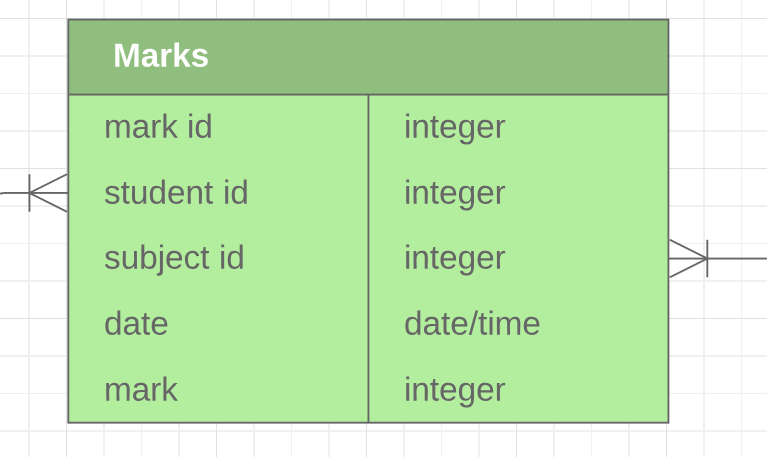
\includegraphics{01-img/1.png}
\caption{This is a entity.}
\end{figure}

My example is a table called \texttt{Marks}, which has
\texttt{mark\ id}, \texttt{student\ id}, \texttt{subject\ id},
\texttt{date} and \texttt{mark} as attributes. The other column is the
variable's type.

\subsubsection{Atributte}\label{atributte}

An attribute is a feature we want to keep track.

\subsubsection{Relationship}\label{relationship}

Is a way to connect two tables.

\begin{figure}
\centering
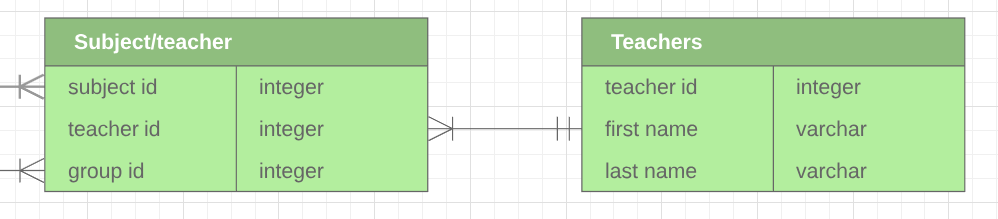
\includegraphics{01-img/2.png}
\caption{The line connecting two tables is a relationship.}
\end{figure}

Remember, this line has some properties, that is named as cardinality.

\subsubsection{Cardinality}\label{cardinality}

Cardinality represents a notation of how the information between tables
will interact with each other.

\begin{figure}
\centering
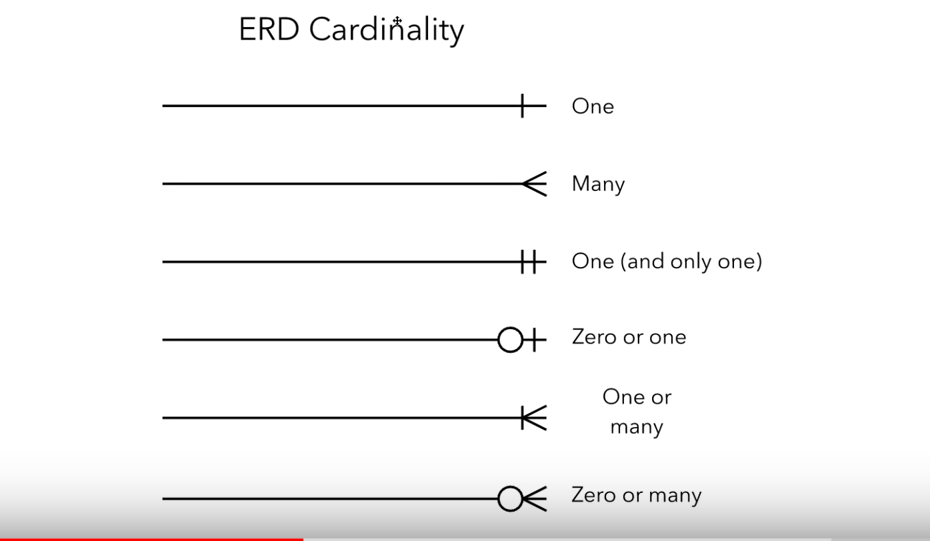
\includegraphics{01-img/3.png}
\caption{In a nutshell of Cardinality - Extracted from the Lucidchart
Video.}
\end{figure}

Additional videos with good content.

\href{https://www.youtube.com/watch?v=QpdhBUYk7Kk\&vl=en}{Video 1 -
Lucidchart} \href{https://www.youtube.com/watch?v=-CuY5ADwn24}{Vídeo 2 -
Lucidchart}

\begin{center}\rule{0.5\linewidth}{\linethickness}\end{center}

\subsection{SQL Introduction}\label{sql-introduction}

SQL is a Language used to manage this interactions between tables,
allowing us to access the stored database. The meaning of SQL is:

\begin{quote}
Structured Query Language
\end{quote}

It is very popular in Data Analysis because:

\begin{itemize}
\tightlist
\item
  Easy to understand
\item
  Easy to learn
\item
  Used to access very large datasets directly where is stored
\item
  Easy to audit and replicate
\item
  It is possible to run multiple queries at onde
\item
  Almost do not have a limit of rows/observations
\item
  Ensure the data Integrity, it is not possible to register a half child
  if you have defined this field as an integer
\item
  SQL is very fast
\item
  Database provide the data sharing, everybody could access the data
  simultaneously, which is good due to a standardization of database
\end{itemize}

SQL provides also functions such as:

\begin{itemize}
\tightlist
\item
  Summation
\item
  Count
\item
  Max and min
\item
  Mean, etc.
\end{itemize}

Have in mind, probably we are going to manipulate data, and rarely
updating or change values.

SQL is not case sensitive, so the best practices is to write the
clauses/staments in upper case.

\textbf{Best practices}

\begin{Shaded}
\begin{Highlighting}[]
\KeywordTok{SELECT}\NormalTok{ first_column}
  \KeywordTok{FROM}\NormalTok{ my_table}
\end{Highlighting}
\end{Shaded}

\textbf{Bad one}

\begin{Shaded}
\begin{Highlighting}[]
\KeywordTok{SelecT}\NormalTok{ first_column}
\KeywordTok{from}\NormalTok{ my_table}
\end{Highlighting}
\end{Shaded}

Bear in mind, the indentation is not a requirements but helps a lot to
understand your code.

\subsubsection{SQL vs.~NoSQL}\label{sql-vs.nosql}

Extracted from the class notes.

\begin{quote}
You may have heard of NoSQL, which stands for not only SQL. Databases
using NoSQL allow for you to write code that interacts with the data a
bit differently than what we will do in this course. These NoSQL
environments tend to be particularly popular for web based data, but
less popular for data that lives in spreadsheets the way we have been
analyzing data up to this point. One of the most popular NoSQL languages
is called MongoDB. Udacity has a full course on MongoDB that you can
take for free here, but these will not be a focus of this program. NoSQL
is not a focus of analyzing data in this Nanodegree program, but you
might see it referenced outside this course!
\end{quote}

\subsection{Clauses}\label{clauses}

Tell the database what to do.

\subsubsection{\texorpdfstring{\texttt{DROP\ TABLE}}{DROP TABLE}}\label{drop-table}

Remove a table from the database.

\subsubsection{\texorpdfstring{\texttt{CREATE\ TABLE}}{CREATE TABLE}}\label{create-table}

Create a new table.

\subsubsection{\texorpdfstring{\texttt{SELECT}}{SELECT}}\label{select}

Is also know as query, is used to create a new table with the selected
variables. You can use \texttt{*} if you want to select all columns.

\begin{Shaded}
\begin{Highlighting}[]
\KeywordTok{SELECT}\NormalTok{ first_column, second_column, last_column}
  \KeywordTok{FROM}\NormalTok{ first_table;}
\end{Highlighting}
\end{Shaded}

\subsubsection{\texorpdfstring{\texttt{LIMIT}}{LIMIT}}\label{limit}

This is the same of \texttt{.head()} but this could only load a few
lines to analyses the table.

\begin{Shaded}
\begin{Highlighting}[]
\KeywordTok{SELECT}\NormalTok{ first_column}
  \KeywordTok{FROM}\NormalTok{ my_table}
\KeywordTok{LIMIT} \DecValTok{1000}            \CommentTok{/* Will load the firs 1000 lines*/}
\end{Highlighting}
\end{Shaded}

\subsubsection{\texorpdfstring{\texttt{ORDER\ BY}}{ORDER BY}}\label{order-by}

It is possible to order by in ascendant and descendent way.

\textbf{ascendant}

\begin{Shaded}
\begin{Highlighting}[]
\KeywordTok{SELECT}\NormalTok{ first_column, second_column, last_column}
  \KeywordTok{FROM}\NormalTok{ my_table}
\KeywordTok{ORDER} \KeywordTok{BY}\NormalTok{ last_column }\CommentTok{/*ascendanting*/}
\KeywordTok{LIMIT} \DecValTok{1000}
\end{Highlighting}
\end{Shaded}

\textbf{descendent}

\begin{Shaded}
\begin{Highlighting}[]
\KeywordTok{SELECT}\NormalTok{ first_column, second_column, last_column}
  \KeywordTok{FROM}\NormalTok{ my_table}
\KeywordTok{ORDER} \KeywordTok{BY}\NormalTok{ last_column }\KeywordTok{DESC}\NormalTok{, second_column }\CommentTok{/*descending for last_column*/}
\KeywordTok{LIMIT} \DecValTok{1000}
\end{Highlighting}
\end{Shaded}

This last query will returns:

\begin{itemize}
\tightlist
\item
  Last\_column ordered by the highest to lowest;
\item
  The second\_column will be the lowest to highest.
\end{itemize}

\subsubsection{\texorpdfstring{\texttt{WHERE}}{WHERE}}\label{where}

Apply a filter to find a specific customer or anything else.

\begin{Shaded}
\begin{Highlighting}[]
\KeywordTok{SELECT}\NormalTok{ first_column, second_column, last_column}
  \KeywordTok{FROM}\NormalTok{ my_table}
\KeywordTok{WHERE}\NormalTok{ first_column = }\DecValTok{100}
\KeywordTok{ORDER} \KeywordTok{BY}\NormalTok{ second_column}
\KeywordTok{LIMIT} \DecValTok{100}
\end{Highlighting}
\end{Shaded}

All staments possible to use. * \texttt{\textgreater{}} (greater than) *
\texttt{\textless{}} (less than) * \texttt{\textgreater{}=} (greater
than or equal to) * \texttt{\textless{}=} (less than or equal to) *
\texttt{=} (equal to) * \texttt{!=} (not equal to)

If the argument of the WHERE clause is not a number, you must use single
quotes.

\begin{Shaded}
\begin{Highlighting}[]
\KeywordTok{SELECT}\NormalTok{ first_column, second_column, last_column}
  \KeywordTok{FROM}\NormalTok{ my_table}
\KeywordTok{WHERE}\NormalTok{ first_column = }\StringTok{'Hello World!'}
\KeywordTok{ORDER} \KeywordTok{BY}\NormalTok{ second_column}
\KeywordTok{LIMIT} \DecValTok{100}
\end{Highlighting}
\end{Shaded}

\subsection{Derived Columns}\label{derived-columns}

Is a new column created from the query. It is similar to the
\texttt{mutate} function from R.

This is the operator to create a derived column:

\begin{itemize}
\tightlist
\item
  \texttt{*} (Multiplication)
\item
  \texttt{+} (Addition)
\item
  \texttt{-} (Subtraction)
\item
  \texttt{/} (Division)
\end{itemize}

\begin{Shaded}
\begin{Highlighting}[]
\KeywordTok{SELECT} \KeywordTok{id}\NormalTok{, (standard_amt_usd/total_amt_usd)*}\DecValTok{100}
\KeywordTok{FROM}\NormalTok{ orders}
\KeywordTok{LIMIT} \DecValTok{10}\NormalTok{;}
\end{Highlighting}
\end{Shaded}

Will display without a specific name (?column?).

\subsubsection{\texorpdfstring{\texttt{AS}}{AS}}\label{as}

If you use the \texttt{AS} the derived column will be name as you define
(in other words ``alias'').

\begin{Shaded}
\begin{Highlighting}[]
\KeywordTok{SELECT} \KeywordTok{id}\NormalTok{, (standard_amt_usd/total_amt_usd)*}\DecValTok{100} \KeywordTok{AS}\NormalTok{ std_percent, total_amt_usd}
\KeywordTok{FROM}\NormalTok{ orders}
\KeywordTok{LIMIT} \DecValTok{10}\NormalTok{;}
\end{Highlighting}
\end{Shaded}

Best pratices: No capital letters, descriptive names, etc.

\subsection{\texorpdfstring{Introduction to ``Logical
Operators''}{Introduction to Logical Operators}}\label{introduction-to-logical-operators}

In the next concepts, you will be learning about Logical Operators.
Logical Operators include:

\subsubsection{LIKE}\label{like}

Using with WHERE clause could search some patterns.

\begin{Shaded}
\begin{Highlighting}[]
\KeywordTok{SELECT}\NormalTok{ first_column, second_column, last_column}
  \KeywordTok{FROM}\NormalTok{ my_table}
\KeywordTok{WHERE}\NormalTok{ last_column }\KeywordTok{LIKE} \StringTok{'%ello%'}
\end{Highlighting}
\end{Shaded}

The \texttt{\%} is called wild-card.

\subsubsection{IN}\label{in}

It is the same in Python or R. \texttt{IN} will be used to filter the
dataset based on a list.

\begin{Shaded}
\begin{Highlighting}[]
\KeywordTok{SELECT}\NormalTok{ first_column, second_column, last_column}
  \KeywordTok{FROM}\NormalTok{ my_table}
\KeywordTok{WHERE}\NormalTok{ last_column }\KeywordTok{IN}\NormalTok{ (}\DecValTok{100}\NormalTok{, }\DecValTok{200}\NormalTok{)}
\end{Highlighting}
\end{Shaded}

This example will filter the rows of last\_column with values of 100 or
200.

\subsubsection{NOT}\label{not}

\texttt{NOT} return the reverse/opposite.

\begin{Shaded}
\begin{Highlighting}[]
\KeywordTok{SELECT}\NormalTok{ first_column, second_column, last_column}
  \KeywordTok{FROM}\NormalTok{ my_table}
\KeywordTok{WHERE}\NormalTok{ last_column }\KeywordTok{NOT} \KeywordTok{IN}\NormalTok{ (}\DecValTok{100}\NormalTok{, }\DecValTok{200}\NormalTok{)}
\end{Highlighting}
\end{Shaded}

This example will remove all observations equals to 100 or 200.

Possible uses:

\begin{itemize}
\tightlist
\item
  NOT IN
\item
  NOT LIKE
\end{itemize}

\subsubsection{AND}\label{and}

Logical statment usually to make some filtration.

\begin{Shaded}
\begin{Highlighting}[]
\KeywordTok{SELECT}\NormalTok{ *}
\KeywordTok{FROM}\NormalTok{ orders}
\KeywordTok{WHERE}\NormalTok{ standard_qty > }\DecValTok{1000} \KeywordTok{AND}\NormalTok{ poster_qty = }\DecValTok{0} \KeywordTok{AND}\NormalTok{ gloss_qty = }\DecValTok{0}\NormalTok{;}
\end{Highlighting}
\end{Shaded}

\subsubsection{BETWEEN}\label{between}

Sometimes AND statment could be replaced by BETWEEN, this is much
clearly to understand. BUT the BETWEEN is inclusive, which means the
endpoints will be included in the filter.

\begin{Shaded}
\begin{Highlighting}[]
\KeywordTok{SELECT}\NormalTok{ name}
\KeywordTok{FROM}\NormalTok{ accounts}
\KeywordTok{WHERE}\NormalTok{ name }\KeywordTok{NOT} \KeywordTok{LIKE} \StringTok{'C%'} \KeywordTok{AND}\NormalTok{ name }\KeywordTok{LIKE} \StringTok{'%s'}\NormalTok{;}
\end{Highlighting}
\end{Shaded}

\subsubsection{OR}\label{or}

Well, this is a logical operator.

\begin{Shaded}
\begin{Highlighting}[]
\KeywordTok{SELECT} \KeywordTok{id}
\KeywordTok{FROM}\NormalTok{ orders}
\KeywordTok{WHERE}\NormalTok{ gloss_qty > }\DecValTok{4000} \KeywordTok{OR}\NormalTok{ poster_qty > }\DecValTok{4000}\NormalTok{;}
\end{Highlighting}
\end{Shaded}

\section{SQL Joins}\label{sql-joins}

\subsection{Joins}\label{joins}

When a table is splited the performance to update or just to make a
query is better than a big one. The reason is the quantity of data to
read. This is one of the reason to split dataset in several tables, even
more, sometimes in convinient to split because the type of data stored.

The reason of JOIN is to ``bind'' two datasets into one. Here we need to
use the period \texttt{.} (table.colums) to reference which
column/variable we want to select.

\begin{Shaded}
\begin{Highlighting}[]
\KeywordTok{SELECT}\NormalTok{ accounts.name, orders.occurred_at}
  \KeywordTok{FROM}\NormalTok{ orders}
\KeywordTok{JOIN}\NormalTok{ accounts}
\KeywordTok{ON}\NormalTok{ orders.account_id = accounts.id;}
\end{Highlighting}
\end{Shaded}

The result of this query is two columns (\texttt{name} and
\texttt{occured\_at}), and to linked by the \texttt{account\_id} and
\texttt{id}.

\subsubsection{Primary Key (PK)}\label{primary-key-pk}

Is a columns with unique values used to map a variable.

\subsubsection{Foreign Key (FK)}\label{foreign-key-fk}

Is a Primary Key from the other table. We use the PK and FK to link the
tables.

Based on the new information about \texttt{PK} and \texttt{FK}. Let's
insert a picture to visualize the database.

\begin{figure}
\centering
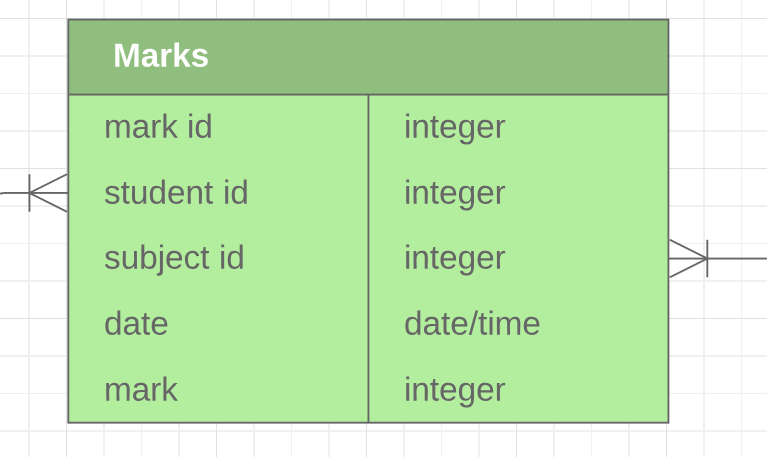
\includegraphics{01-img/1.png}
\caption{Example of Join}
\end{figure}

I want to Join these tables. My query:

\begin{Shaded}
\begin{Highlighting}[]
\KeywordTok{SELECT}\NormalTok{ orders.*}
\KeywordTok{FROM}\NormalTok{ orders}
\KeywordTok{JOIN}\NormalTok{ accounts}
\KeywordTok{ON}\NormalTok{ orders.account_id = accounts.id;}
\end{Highlighting}
\end{Shaded}

What I need to realize:

\begin{itemize}
\tightlist
\item
  \texttt{PK} and \texttt{FK} \textbf{always} will be allocated in
  \texttt{ON}.
\item
  \texttt{FROM} and \texttt{JOIN} each one with one table.
\end{itemize}

\subsubsection{Binding three tables}\label{binding-three-tables}

It is possible to ``chaining'' three tables.

\begin{Shaded}
\begin{Highlighting}[]
\KeywordTok{SELECT}\NormalTok{ *}
\KeywordTok{FROM}\NormalTok{ web_events}
\KeywordTok{JOIN}\NormalTok{ accounts}
\KeywordTok{ON}\NormalTok{ web_events.account_id = accounts.id}
\KeywordTok{JOIN}\NormalTok{ orders}
\KeywordTok{ON}\NormalTok{ accounts.id = orders.account_id}
\end{Highlighting}
\end{Shaded}

In this case, I will import all columns, but I may want few columns.

\begin{Shaded}
\begin{Highlighting}[]
\KeywordTok{SELECT}\NormalTok{ web_events.channel, accounts.name, orders.total}
\KeywordTok{FROM}\NormalTok{ web_events}
\KeywordTok{JOIN}\NormalTok{ accounts}
\KeywordTok{ON}\NormalTok{ web_events.account_id = accounts.id}
\KeywordTok{JOIN}\NormalTok{ orders}
\KeywordTok{ON}\NormalTok{ accounts.id = orders.account_id}
\end{Highlighting}
\end{Shaded}

\subsubsection{Alias}\label{alias}

Alias is a form to ``short'' the name of columns, the first method is
using \texttt{AS}, but it could be simplified by only a space.

\begin{itemize}
\tightlist
\item
  Example 1
\end{itemize}

\begin{Shaded}
\begin{Highlighting}[]
\KeywordTok{Select}\NormalTok{ t1.column1 aliasname, t2.column2 aliasname2}
\KeywordTok{FROM}\NormalTok{ tablename }\KeywordTok{AS}\NormalTok{ t1}
\KeywordTok{JOIN}\NormalTok{ tablename2 }\KeywordTok{AS}\NormalTok{ t2}
\end{Highlighting}
\end{Shaded}

\textbf{or}

\begin{Shaded}
\begin{Highlighting}[]
\KeywordTok{Select}\NormalTok{ t1.column1 aliasname, t2.column2 aliasname2}
\KeywordTok{FROM}\NormalTok{ tablename t1}
\KeywordTok{JOIN}\NormalTok{ tablename2 t2}
\end{Highlighting}
\end{Shaded}

\begin{itemize}
\tightlist
\item
  Example 2
\end{itemize}

\begin{Shaded}
\begin{Highlighting}[]
\KeywordTok{SELECT}\NormalTok{ col1 + col2 }\KeywordTok{AS}\NormalTok{ total, col3}
\end{Highlighting}
\end{Shaded}

\textbf{or}

\begin{Shaded}
\begin{Highlighting}[]
\KeywordTok{SELECT}\NormalTok{ col1 + col2 total, col3}
\end{Highlighting}
\end{Shaded}

\textbf{or}

\subsubsection{\texorpdfstring{\texttt{INNER\ JOIN}}{INNER JOIN}}\label{inner-join}

Returns rows which appears in both tables.

\begin{Shaded}
\begin{Highlighting}[]
\KeywordTok{SELECT}\NormalTok{ table_1.id, table_1.name, table_2.total}
  \KeywordTok{FROM}\NormalTok{ table_}\DecValTok{2}
    \KeywordTok{JOIN}\NormalTok{ table_}\DecValTok{1}
      \KeywordTok{ON}\NormalTok{ table_2.account_id = table_1.id}
\end{Highlighting}
\end{Shaded}

These last examples are all \texttt{INNER\ JOINS}, and will return a new
dataframe (intersection between two dataframes).

\subsubsection{\texorpdfstring{\texttt{OUTER\ JOIN}}{OUTER JOIN}}\label{outer-join}

There are two kinds of OUTER JOINs

\begin{itemize}
\tightlist
\item
  Left outer JOIN, and;
\item
  Right outer JOIN.
\end{itemize}

This two new JOINs has a property to pull rows that only exist in one
table, it means some rows might have NULL values. The standard for this
course will be to use only the left outer join.

\section{SQL Aggregations}\label{sql-aggregations}

\subsection{Aggregations Functions}\label{aggregations-functions}

This is functions return a single row with the aggregated value.

\begin{itemize}
\tightlist
\item
  sum;
\item
  min;
\item
  max;
\item
  mean, etc.
\end{itemize}

\subsubsection{NULL}\label{null}

NULL is no a value, it is different from ZERO or a space, for this
reason you can not use equal (\texttt{=}) to find it, for do so you must
use \texttt{IS}. The NULL is ignored in all aggregatins functions, and
it is defined as a property of the data.

For the \emph{Parch and Posey} dataset, NULL is equal to zero.

\begin{Shaded}
\begin{Highlighting}[]
\KeywordTok{WHERE}\NormalTok{ something }\KeywordTok{IS} \KeywordTok{NULL}
\KeywordTok{WHERE}\NormalTok{ something }\KeywordTok{IS} \KeywordTok{NOT} \KeywordTok{NULL}
\end{Highlighting}
\end{Shaded}

\paragraph{NULLs - Expert Tip}\label{nulls---expert-tip}

There are two common ways in which you are likely to encounter NULLs:

\begin{itemize}
\tightlist
\item
  NULLs frequently occur when performing a LEFT or RIGHT JOIN. You saw
  in the last lesson - when some rows in the left table of a left join
  are not matched with rows in the right table, those rows will contain
  some NULL values in the result set.
\item
  NULLs can also occur from simply missing data in our database.
\end{itemize}

\subsection{Functions}\label{functions}

\subsubsection{COUNT()}\label{count}

Count the number of rows. If the entire line has only NULLs, this line
will be noted counted.

Simple Example:

\begin{Shaded}
\begin{Highlighting}[]
\KeywordTok{SELECT} \FunctionTok{COUNT}\NormalTok{(*)}
\KeywordTok{FROM}\NormalTok{ accounts;}
\end{Highlighting}
\end{Shaded}

Example with filter

\begin{Shaded}
\begin{Highlighting}[]
\KeywordTok{SELECT} \FunctionTok{COUNT}\NormalTok{(*) }\KeywordTok{AS}\NormalTok{ order_count}
\KeywordTok{FROM}\NormalTok{ some_table}
\KeywordTok{WHERE}\NormalTok{ any_column > }\DecValTok{100} \KeywordTok{AND}\NormalTok{ any_column < }\DecValTok{200}\NormalTok{;}
\end{Highlighting}
\end{Shaded}

Example with column selection

\begin{Shaded}
\begin{Highlighting}[]
\KeywordTok{SELECT} \FunctionTok{COUNT}\NormalTok{(account.id)}
\KeywordTok{FROM}\NormalTok{ accounts;}
\end{Highlighting}
\end{Shaded}

\subsubsection{SUM()}\label{sum}

Perform the summation among rows. You must define which columns will be
applied the sum function.

\begin{Shaded}
\begin{Highlighting}[]
\KeywordTok{SELECT} \FunctionTok{SUM}\NormalTok{(poster_qty)}
\KeywordTok{FROM}\NormalTok{ demo.orders;}
\end{Highlighting}
\end{Shaded}

\subsubsection{MAX() and MIN()}\label{max-and-min}

Return a rows with the minimun or maximum of a given column.

\begin{Shaded}
\begin{Highlighting}[]
\KeywordTok{SELECT} \FunctionTok{MAX}\NormalTok{(poster_qty) }\KeywordTok{AS}\NormalTok{ max_poster_qty,}
       \FunctionTok{MIN}\NormalTok{(standard_qty) }\KeywordTok{AS}\NormalTok{ min_standard_qty}
\KeywordTok{FROM}\NormalTok{ demo.orders;}
\end{Highlighting}
\end{Shaded}

\subsubsection{GROUP BY}\label{group-by}

Divide the non-grouped column into groups, which means the aggregated
function will be calculated by group.

\begin{itemize}
\tightlist
\item
  The GROUP BY always goes between WHERE and ORDER BY.
\end{itemize}

Example 1:

\begin{Shaded}
\begin{Highlighting}[]
\KeywordTok{SELECT}\NormalTok{ a.name, o.occurred_at}
\KeywordTok{FROM}\NormalTok{ accounts a}
\KeywordTok{JOIN}\NormalTok{ orders o}
\KeywordTok{ON}\NormalTok{ a.id = o.account_id}
\KeywordTok{ORDER} \KeywordTok{BY}\NormalTok{ o.occurred_at}
\KeywordTok{LIMIT} \DecValTok{1}\NormalTok{;}
\end{Highlighting}
\end{Shaded}

Same example but indexing by number:

\begin{Shaded}
\begin{Highlighting}[]
\KeywordTok{SELECT}\NormalTok{ a.name, o.occurred_at}
\KeywordTok{FROM}\NormalTok{ accounts a}
\KeywordTok{JOIN}\NormalTok{ orders o}
\KeywordTok{ON}\NormalTok{ a.id = o.account_id}
\KeywordTok{ORDER} \KeywordTok{BY} \DecValTok{2}
\KeywordTok{LIMIT} \DecValTok{1}\NormalTok{;}
\end{Highlighting}
\end{Shaded}

\emph{OBS.: The index used in ORDER BY clause is to refence
o.occurred\_at.}

\subsubsection{DISTINCT}\label{distinct}

DISTINCT is always used in SELECT statements, and it provides the unique
rows for all columns written in the SELECT statement. Therefore, you
only use DISTINCT once in any particular SELECT statement.

\begin{Shaded}
\begin{Highlighting}[]
\KeywordTok{SELECT} \KeywordTok{DISTINCT}\NormalTok{ column1, column2, column3}
\KeywordTok{FROM}\NormalTok{ table1;}
\end{Highlighting}
\end{Shaded}

\subsubsection{HAVING}\label{having}

\begin{quote}
HAVING is the ``clean'' way to filter a query that has been aggregated,
but this is also commonly done using a subquery. Essentially, any time
you want to perform a WHERE on an element of your query that was created
by an aggregate, you need to use HAVING instead.
\end{quote}

Note extracted from the class notes.

\begin{Shaded}
\begin{Highlighting}[]
\KeywordTok{SELECT}\NormalTok{ s.id, s.name, }\FunctionTok{COUNT}\NormalTok{(*) num_accounts}
\KeywordTok{FROM}\NormalTok{ accounts a}
\KeywordTok{JOIN}\NormalTok{ sales_reps s}
\KeywordTok{ON}\NormalTok{ s.id = a.sales_rep_id}
\KeywordTok{GROUP} \KeywordTok{BY}\NormalTok{ s.id, s.name}
\KeywordTok{HAVING} \FunctionTok{COUNT}\NormalTok{(*) > }\DecValTok{5}
\KeywordTok{ORDER} \KeywordTok{BY}\NormalTok{ num_accounts;}
\end{Highlighting}
\end{Shaded}

\subsection{DATE}\label{date}

To GROUP BY a date is quite complicated because each time is (obviously)
different, for this, reason is necessary to ``round'' the time/date to
group them.

\subsubsection{DATE\_TRUNC}\label{date_trunc}

Common trunctions are:

\begin{itemize}
\tightlist
\item
  day;
\item
  month, and;
\item
  year.
\end{itemize}

Sintaxe:

DATE\_TRUNC(`{[}interval{]}', time\_column)

Where:

\begin{itemize}
\tightlist
\item
  microsecond
\item
  millisecond
\item
  second
\item
  minute
\item
  hour
\item
  day
\item
  week
\item
  month
\item
  quarter
\item
  year
\item
  century
\item
  decade
\item
  millenium
\end{itemize}

For further explanaition about
\href{https://blog.modeanalytics.com/date-trunc-sql-timestamp-function-count-on/}{date}

\begin{Shaded}
\begin{Highlighting}[]
\KeywordTok{SELECT}\NormalTok{ demo.accounts.name,}
\NormalTok{       DATE_TRUNC(}\StringTok{'month'}\NormalTok{, demo.orders.occurred_at) }\KeywordTok{AS}\NormalTok{ year_month,}
       \FunctionTok{SUM}\NormalTok{(demo.orders.gloss_amt_usd) }\KeywordTok{AS}\NormalTok{ sum_gloss_usd}
\KeywordTok{FROM}\NormalTok{ demo.orders}
\KeywordTok{JOIN}\NormalTok{ demo.accounts}
\KeywordTok{ON}\NormalTok{ demo.orders.account_id = demo.accounts.id}
\KeywordTok{WHERE}\NormalTok{ demo.accounts.name = }\StringTok{'Walmart'}
\KeywordTok{GROUP} \KeywordTok{BY}\NormalTok{ year_month, demo.accounts.name}
\KeywordTok{ORDER} \KeywordTok{BY}\NormalTok{ sum_gloss_usd }\KeywordTok{DESC}
\KeywordTok{LIMIT} \DecValTok{1}\NormalTok{;}
\end{Highlighting}
\end{Shaded}

\subsubsection{DATE PART}\label{date-part}

Extract part of the date

\subsection{CASE}\label{case}

Create a new column, derivate column, with a kind classification (assign
a value into this new column according to the statment).

\begin{Shaded}
\begin{Highlighting}[]
\KeywordTok{SELECT}\NormalTok{ account_id,}
\NormalTok{       occurred_at,}
\NormalTok{       total,}
       \KeywordTok{CASE} \KeywordTok{WHEN}\NormalTok{ total > }\DecValTok{500} \KeywordTok{THEN} \StringTok{'Over 500'}
            \KeywordTok{WHEN}\NormalTok{ total > }\DecValTok{300} \KeywordTok{AND}\NormalTok{ total <= }\DecValTok{500} \KeywordTok{THEN} \StringTok{'301 - 500'}
            \KeywordTok{WHEN}\NormalTok{ total > }\DecValTok{100} \KeywordTok{AND}\NormalTok{ total <= }\DecValTok{300} \KeywordTok{THEN} \StringTok{'101 - 300'}
            \KeywordTok{ELSE} \StringTok{'100 or under'} \KeywordTok{END} \KeywordTok{AS}\NormalTok{ total_group}
\KeywordTok{FROM}\NormalTok{ demo.orders}
\KeywordTok{LIMIT} \DecValTok{10}\NormalTok{;}
\end{Highlighting}
\end{Shaded}

Creates the total\_group column.

\subsubsection{With AGGREGATION}\label{with-aggregation}

Combining the CASE clause with aggregations function could be a power
tool, because the WHERE clause only evaluate one statement, using WHEN
CASE it is possible to evaluate several staments.

\begin{Shaded}
\begin{Highlighting}[]
\KeywordTok{SELECT}\NormalTok{ demo.orders.account_id,}
\NormalTok{       demo.orders.total_amt_usd,}
       \KeywordTok{CASE} \KeywordTok{WHEN}\NormalTok{ demo.orders.total_amt_usd >= }\DecValTok{3000} \KeywordTok{THEN} \StringTok{'Large'}
            \KeywordTok{ELSE} \StringTok{'Small'} \KeywordTok{END} \KeywordTok{AS} \KeywordTok{level}
\KeywordTok{FROM}\NormalTok{ demo.orders}
\KeywordTok{LIMIT} \DecValTok{10}\NormalTok{;}
\end{Highlighting}
\end{Shaded}

\section{SQL Subqueries \& Temporary Tables
(Advanced)}\label{sql-subqueries-temporary-tables-advanced}

\subsection{Subqueries}\label{subqueries}

This is a way to nest queries, it means: The result of one query will be
used as FROM to the next query.

\begin{Shaded}
\begin{Highlighting}[]
\KeywordTok{SELECT}\NormalTok{ *}
\KeywordTok{FROM}\NormalTok{(}\KeywordTok{SELECT}\NormalTok{ something}
     \KeywordTok{FROM}\NormalTok{   interesting) }\KeywordTok{AS}\NormalTok{ table_}\DecValTok{1}
\end{Highlighting}
\end{Shaded}

In the example above, I have one query nested to another. Bear in mind,
I must give a alias to the nested query.

If the result of the subquery is a single value, you are allowed to
insert this subquery wherever you want.

\subsection{WITH}\label{with}

Also known as \emph{Common Table Expression} (CTE), is a kinf of
subquery but could be more helpful if someone is going to read the code.
Due to the possibility to write the code in fragments an assign name,
this is very handy.

\textbf{Example}

\begin{Shaded}
\begin{Highlighting}[]
\KeywordTok{WITH}\NormalTok{ my_with_example }\KeywordTok{AS}\NormalTok{ (}\KeywordTok{SELECT}\NormalTok{ ... MY CODE)}

\KeywordTok{SELECT}\NormalTok{ something}
\KeywordTok{FROM}\NormalTok{ my_with_example}
\end{Highlighting}
\end{Shaded}

As you can see it provide a better way to code because the code became
more readable.

\section{Data Cleaning (Advanced)}\label{data-cleaning-advanced}

\subsection{Data Cleaning}\label{data-cleaning}

\subsubsection{LEFT and RIGHT}\label{left-and-right}

It is the same of Excel functions.

\begin{Shaded}
\begin{Highlighting}[]
\KeywordTok{SELECT} \KeywordTok{LEFT}\NormalTok{(}\DecValTok{2}\NormalTok{, something) }\KeywordTok{AS}\NormalTok{ lefty_part_of_simething}
\KeywordTok{FROM}\NormalTok{ interesting}
\end{Highlighting}
\end{Shaded}

The example above will create a new column with the first two, from the
left to right, character of something.

\begin{Shaded}
\begin{Highlighting}[]
\KeywordTok{SELECT} \KeywordTok{RIGHT}\NormalTok{(}\DecValTok{2}\NormalTok{, something) }\KeywordTok{AS}\NormalTok{ lefty_part_of_simething}
\KeywordTok{FROM}\NormalTok{ interesting}
\end{Highlighting}
\end{Shaded}

Almost the same, but start from the right to the left.

\subsubsection{LEN}\label{len}

Returns the string length.

\begin{Shaded}
\begin{Highlighting}[]
\KeywordTok{SELECT}\NormalTok{ LEN(something)}
\KeywordTok{FROM}\NormalTok{ interesting}
\end{Highlighting}
\end{Shaded}

\subsubsection{POSITION and STRPOS}\label{position-and-strpos}

POSITION will find a pattern in the string and will return the position
(from the left to the right).

\begin{Shaded}
\begin{Highlighting}[]
\KeywordTok{SELECT}\NormalTok{ POSITION(}\StringTok{','}\NormalTok{, something) }\CommentTok{/*Looking for a coma*/}
\KeywordTok{FROM}\NormalTok{ interesting}
\end{Highlighting}
\end{Shaded}

The STRPOS has the same use and same results.

\begin{Shaded}
\begin{Highlighting}[]
\KeywordTok{SELECT}\NormalTok{ STRPOS(something, }\StringTok{','}\NormalTok{) }\CommentTok{/*Looking for a coma*/}
\KeywordTok{FROM}\NormalTok{ interesting}
\end{Highlighting}
\end{Shaded}

Both functions are case sensitive.

\subsubsection{LOWER and UPPER}\label{lower-and-upper}

Converts string into all lower or all upper cases.

\begin{Shaded}
\begin{Highlighting}[]
\KeywordTok{SELECT} \FunctionTok{LOWER}\NormalTok{(something)}
\KeywordTok{FROM}\NormalTok{ interesting}
\end{Highlighting}
\end{Shaded}

\subsubsection{CONCAT}\label{concat}

Bind/Combine/Concatenate strings (in different) columns into a new
column.

\textbf{Example 1}

\begin{Shaded}
\begin{Highlighting}[]
\KeywordTok{SELECT} \FunctionTok{CONCAT}\NormalTok{(first_name, }\StringTok{' '}\NormalTok{,last_name) }\KeywordTok{AS}\NormalTok{ complete_name }\CommentTok{/* The ' ' is the space between strings*/}
\KeywordTok{FROM}\NormalTok{ interesting}
\end{Highlighting}
\end{Shaded}

You can use \textbar{}\textbar{}.

\textbf{Example 2}

\begin{Shaded}
\begin{Highlighting}[]
\KeywordTok{SELECT}\NormalTok{ first_name || }\StringTok{' '}\NormalTok{ || last_name }\KeywordTok{AS}\NormalTok{ complete_name }\CommentTok{/* The ' ' is the space between strings*/}
\KeywordTok{FROM}\NormalTok{ interesting}
\end{Highlighting}
\end{Shaded}

\subsubsection{CAST}\label{cast}

CAST allow to convert one type to another.

\textbf{Example 1}

\begin{Shaded}
\begin{Highlighting}[]
\KeywordTok{SELECT} \FunctionTok{CAST}\NormalTok{(}\DataTypeTok{year}\NormalTok{ || }\DataTypeTok{month}\NormalTok{ || }\DataTypeTok{day} \KeywordTok{AS} \DataTypeTok{date}\NormalTok{) }\KeywordTok{AS}\NormalTok{ formatted_date}
\KeywordTok{FROM}\NormalTok{ interesting}
\end{Highlighting}
\end{Shaded}

The same of Example 1, but with a different notation to CAST clause.

\textbf{Example 2:}

\begin{Shaded}
\begin{Highlighting}[]
\KeywordTok{SELECT}\NormalTok{ (}\DataTypeTok{year}\NormalTok{ || }\DataTypeTok{month}\NormalTok{ || }\DataTypeTok{day} \KeywordTok{AS} \DataTypeTok{date}\NormalTok{):}\CharTok{:date} \KeywordTok{AS}\NormalTok{ formatted_date}
\KeywordTok{FROM}\NormalTok{ interesting}
\end{Highlighting}
\end{Shaded}

CAST is useful to converter strings into numbers or dates.

\subsubsection{COALESCE}\label{coalesce}

Converts NULL fields into Zero.

\section{Project 01 - Chinook}\label{project-01---chinook}

Questions

All exercises of this chapter I have stored in the Mode Analytics
platform.

\href{https://modeanalytics.com/ah_uyekita/reports/5e871f63f8b2}{Optional
Questions}

Project Submitted

I have written all the project in Mode Analytics because is a better
place to coding.

\begin{itemize}
\tightlist
\item
  I can perform SQL queries;
\item
  I can create graphics;
\item
  An opportunity to get knowledge in a new tool.
\end{itemize}

\href{https://modeanalytics.com/ah_uyekita/reports/e77643786160}{Project
01 in Mode Analytic}

\begin{center}\rule{0.5\linewidth}{\linethickness}\end{center}

\subsection{Project Submission}\label{project-submission}

To submit your project, please do the following:

\begin{itemize}
\tightlist
\item
  Review your project against the project Rubric. Reviewers will use
  this to evaluate your work.
\item
  Create your slides with whatever presentation software you'd like
  (e.g.~Google Slides, PowerPoint, Keynote, etc.).
\end{itemize}

In order to review your presentation, you will need to save your slides
as a PDF. You can do this from within Google Slides by selecting File
\textgreater{} Download as \textgreater{} PDF Document.

\begin{center}\rule{0.5\linewidth}{\linethickness}\end{center}

\chapter{Data Wrangling}\label{data-wrangling}

Tags

\begin{itemize}
\tightlist
\item
  Author : AH Uyekita
\item
  Title : \emph{Data Wrangling}
\item
  Date : 18/12/2018
\item
  Course : Data Science II - Foundations Nanodegree
\item
  COD : ND111
\end{itemize}

Jupyter Notebooks

\begin{itemize}
\tightlist
\item
  Lesson 01
\item
  Lesson 02
\item
  Lesson 03
\end{itemize}

Outline

\begin{itemize}
\tightlist
\item
  {[}x{]} Lesson 01 - Introduction to Data Wrangling
\item
  {[}x{]} Lesson 02 - Gathering
\item
  {[}x{]} Lesson 03 - Assessing Data
\item
  {[}x{]} Lesson 04 - Cleaning Data
\item
  {[}x{]} Project 02 - Wrangle and Analyze Data
\end{itemize}

\section{Introduction to Data
Wrangling}\label{introduction-to-data-wrangling}

There are roughly three steps in the Data Wrangling.

\begin{itemize}
\tightlist
\item
  Gathering;
\item
  Assessing, and;
\item
  Cleaning.
\end{itemize}

This is a iterate process between these three steps.

\begin{quote}
Data wrangling is about gathering the right pieces of data, assessing
your data's quality and structure, then modifying your data to make it
clean. But the assessments you make and convert to cleaning operations
won't make your analysis, viz, or model better, though. The goal is to
just make them possible, i.e., functional.
\end{quote}

\begin{quote}
EDA is about exploring your data to later augment it to maximize the
potential of our analyses, visualizations, and models. When exploring,
simple visualizations are often used to summarize your data's main
characteristics. From there you can do things like remove outliers and
create new and more descriptive features from existing data, also known
as feature engineering. Or detect and remove outliers so your model's
fit is better.
\end{quote}

\begin{quote}
ETL: You also may have heard of the extract-transform-load process also
known as ETL. ETL differs from data wrangling in three main ways: * The
users are different * The data is different * The use cases are
different This article (Data Wrangling Versus ETL: What's the
Difference?) by Wei Zhang explains these three differences well.
\end{quote}

All text extracted from the class notes.

\subsection{Gathering}\label{gathering}

Gathering is the first step of a Data Wrangling, is also known as
Collecting or Acquiring. The Armenian Online Job Post has 19,000 jobs
postings from 2004 to 2015.

\begin{quote}
Best Practice: Downloading Files Programmatically
\end{quote}

This is the reasons:

\begin{itemize}
\tightlist
\item
  Scalability: This automation will save time, and prevents erros;
\item
  Reproducibility: Key point to any research. Anyone could reproduce
  your work and check it.
\end{itemize}

\subsection{Assessing}\label{assessing}

The assessing in divided into two mains aspects:

\begin{itemize}
\tightlist
\item
  Quality of the dataset
\item
  Tidiness of the dataset
\end{itemize}

\subsubsection{Quality}\label{quality}

Low quality dataset is related to a dirty dataset, which means the
content quality of data.

Commom issues:

\begin{itemize}
\tightlist
\item
  Missing values
\item
  Non standard units (km, meters, inches, etc. all mixed)
\item
  Innacurate data, invalid data, inconsistent data, etc.
\end{itemize}

\begin{quote}
One dataset may be high enough quality for one application but not for
another.
\end{quote}

\subsubsection{Tidiness}\label{tidiness}

Untidy data or \emph{messy} data, is about the structure of the dataset.

\begin{itemize}
\tightlist
\item
  Each obsevation by rows, and;
\item
  Each variable/features by column.
\end{itemize}

This is the Hadley Wickham definition of tidy data.

\subsection{Assessing the data}\label{assessing-the-data}

There are two ways to assess the data.

\begin{itemize}
\tightlist
\item
  Visual, and;
\item
  Programmatic.
\end{itemize}

\subsubsection{Visual Assessment}\label{visual-assessment}

Using regular tools, such as Graphics, Excel, tables, etc. It means,
there is a human assessing the data.

\subsubsection{Programmatic Assessment}\label{programmatic-assessment}

Using automation to dataset evaluation is scalable, and allows you to
handle a very huge quantity of data.

Examples of ``Programmatic Assessment'': Analysing the data using
\texttt{.info()}, \texttt{.head()}, \texttt{.describe()}, plotting
graphics (\texttt{.plot()}), etc..

Bear in mind, in this step we do not use ``verbs'' to describe any
erros/problem, because the ``verbs'' will be actions to the next step.

\subsection{Cleaning}\label{cleaning}

Improving the quality of a dataset or cleaning the dataset do not means:
Changing the data (because it could be \textbf{data fraud}).

The meaning of Cleaning is correcting the data or removing the data.

\begin{itemize}
\tightlist
\item
  Innacurate, wrong or irrelevant data.
\item
  Replacing or filling (NULL or NA values) data.
\item
  Combining/Merging datasets.
\end{itemize}

Improving the tidiness is transform the dataset to follow:

\begin{itemize}
\tightlist
\item
  each observation = row
\item
  each variable = column
\end{itemize}

There are two ways to cleaning the data: manually and programmatic.

\subsubsection{Manually}\label{manually}

To be avoided.

\subsubsection{Programmatic}\label{programmatic}

There are three steps:

\begin{enumerate}
\def\labelenumi{\arabic{enumi}.}
\tightlist
\item
  Define
\item
  Code
\item
  Test
\end{enumerate}

\begin{quote}
\textbf{Defining} means defining a data cleaning plan in writing, where
we turn our assessments into defined cleaning tasks. This plan will also
serve as an instruction list so others (or us in the future) can look at
our work and reproduce it.
\end{quote}

\begin{quote}
\textbf{Coding} means translating these definitions to code and
executing that code.
\end{quote}

\begin{quote}
\textbf{Testing} means testing our dataset, often using code, to make
sure our cleaning operations worked.
\end{quote}

Text from the class notes.

\section{Data Gathering}\label{data-gathering}

This is the first step of any Data Wrangling, sometimes this process is
a bit complicated because you need to find these data (probably from
different sources and then merge).

\subsection{Flat File}\label{flat-file}

This is the way to store data into a single text file, usually, this
file has another extension (.csv, tsv, etc.), each one of this extension
has your own characteristic.

\begin{itemize}
\tightlist
\item
  Each variable/features is separated by a comma and each row is an
  observation;
\item
  Each variable/features is separated by a tab and each row is an
  observation.
\end{itemize}

There are some \textbf{advantages} for using the flat files.

\begin{itemize}
\tightlist
\item
  Anyone could read, even a human;
\item
  Is lightweight;
\item
  You do not need to install a specific software;
\item
  Simple to understand (each variable is delimited by a coma/tab);
\item
  Any software could open it;
\item
  Very good to small dataset.
\end{itemize}

But has disadvantages also:

\begin{itemize}
\tightlist
\item
  Do not have standard;
\item
  Do not have data integrity checks;

  \begin{itemize}
  \tightlist
  \item
    Duplicated rows;
  \item
    You can record any value in any field;
  \end{itemize}
\item
  Not great to large datasets.
\end{itemize}

\paragraph{Importing the tsv file}\label{importing-the-tsv-file}

I have used the \texttt{read\_csv} to load the data, but I have set the
sep argument as \texttt{\textbackslash{}t}, which means tabular.
Sometimes, the flat files use \texttt{;} or \texttt{,}, so it is
necessary to define what is the delimiter.

\textbf{Example:}

\begin{Shaded}
\begin{Highlighting}[]
\ImportTok{import}\NormalTok{ pandas }\ImportTok{as}\NormalTok{ pd}
\NormalTok{df }\OperatorTok{=}\NormalTok{ pd.read_cvs(}\StringTok{'bestofrt.tsv'}\NormalTok{, sep}\OperatorTok{=} \StringTok{'}\CharTok{\textbackslash{}t}\StringTok{'}\NormalTok{)}
\end{Highlighting}
\end{Shaded}

\subsection{Web Scraping}\label{web-scraping}

This is terminology is used to say the data extracted from a website
(usually using code to do it). Due to this code depends on the HTML
file, if any change of the website happens, all the code used to web
scrapping could stopping to working properly, which requires an
adjustments. For this reason, web scraping is not a definitive solution.

\subsection{HTTP Request}\label{http-request}

This is useful to access archives from the internet, combining with the
OS package, it is possible to download and store locally the file.

\subsection{Encoding and Character
Set}\label{encoding-and-character-set}

This explanation is based on
\href{https://stackoverflow.com/questions/6224052/what-is-the-difference-between-a-string-and-a-byte-string}{this}
Stack Overflow thread.

Encoding: Is a proccess to convert a something into bytes.

\begin{itemize}
\tightlist
\item
  Audio is encoded into MP3, WAV, etc.
\item
  Images is encoded into PNG, JPG, TIFF, etc.
\item
  Text files is enconded into ASCII, UTF-8, etc.
\end{itemize}

The Character Set is as the name, is a set of charaters which I can use
to write a phrase, each character has a code which represents the
letter/character. There are several character set such as ASCII and
UTF-8.

\subsection{Application Programming Interfaces -
API}\label{application-programming-interfaces---api}

The API let you access the data from the internet in a resonable easy
manner.

There are several API available in the internet for many social media:

\begin{itemize}
\tightlist
\item
  Facebook;
\item
  Instagram;
\item
  Twitter, etc.;
\end{itemize}

This lesson will use the
\href{https://www.mediawiki.org/wiki/MediaWiki}{Mediawiki}, which is a
Open Source API to Wikipedia.

Most of the file from the API are formated as JSON or XML.

\subsection{JSON and XML}\label{json-and-xml}

JSON stands for Javascript Object Notation and XML for Extensible Markup
Language.

Sometimes the regular tabular way to structure the data is not a good
solution, and for this reason, there are other forms to store data as
JSON and XML.

They use a kind of ``dictionary'' to store data, which allows storing
more than one information per variable.

There are some similarities in JSON and Python:

\begin{itemize}
\tightlist
\item
  JSON Array = Python list
\item
  JSON Object = Python dictonary
\end{itemize}

\subsection{Methods in this Lesson}\label{methods-in-this-lesson}

\subsubsection{\texorpdfstring{\texttt{.find()}}{.find()}}\label{find}

This method is used to find tags and containers.

\textbf{Example:}

\begin{Shaded}
\begin{Highlighting}[]
\NormalTok{soup.find(}\StringTok{'title'}\NormalTok{)}
\end{Highlighting}
\end{Shaded}

This code above will find the tag title, and return the content.

\subsubsection{\texorpdfstring{\texttt{.find\_all()}}{.find\_all()}}\label{find_all}

It is almost the same of \texttt{.find()}, but will find in all document
the given pattern.

\textbf{Example:}

\begin{Shaded}
\begin{Highlighting}[]
\NormalTok{something.find_all(}\StringTok{'div'}\NormalTok{)}
\end{Highlighting}
\end{Shaded}

This code will return all \texttt{div} in the document. It could be used
with \texttt{limit\ =\ 1}, which will return the first \texttt{div}.

\subsubsection{\texorpdfstring{\texttt{.contents}}{.contents}}\label{contents}

The \texttt{.contents} get the elements from the \texttt{find} and
\texttt{find\_all}.You are capable to select, which element you want
(indexing).

\begin{Shaded}
\begin{Highlighting}[]
\NormalTok{something.find_all(}\StringTok{'div'}\NormalTok{)[}\DecValTok{1}\NormalTok{].contents[}\DecValTok{2}\NormalTok{]}
\end{Highlighting}
\end{Shaded}

In this fragment of code, I am selecting only the third element of
\texttt{something.find\_all(\textquotesingle{}div\textquotesingle{}){[}1{]}}.

\subsubsection{\texorpdfstring{\texttt{os.listdir()}}{os.listdir()}}\label{os.listdir}

This function list all files inside a given folder/directory.

\begin{Shaded}
\begin{Highlighting}[]
\NormalTok{os.listdir(my_path)}
\end{Highlighting}
\end{Shaded}

\subsubsection{\texorpdfstring{\texttt{.glob()}}{.glob()}}\label{glob}

This method is a part of the glob package.

If you are familiar with Linux CLI, you have alread used the globbing to
find a file in a folder.

\begin{Shaded}
\begin{Highlighting}[]
\ImportTok{import}\NormalTok{ glob}
\NormalTok{glob.glob(}\StringTok{'any_folder/*.txt'}\NormalTok{)}
\end{Highlighting}
\end{Shaded}

The result of the \texttt{.glob()} will be a list with all files which
matches the \texttt{.txt}.

\subsubsection{\texorpdfstring{\texttt{.read()}}{.read()}}\label{read}

Convert the file into a in memory variable.

\begin{Shaded}
\begin{Highlighting}[]
\NormalTok{my_new_variable }\OperatorTok{=} \BuiltInTok{file}\NormalTok{.read() }\CommentTok{# my_new_variable is a variable which contains the file.}
\end{Highlighting}
\end{Shaded}

\subsubsection{\texorpdfstring{\texttt{.readline()}}{.readline()}}\label{readline}

Read line by line every instance which is used this method.

\begin{Shaded}
\begin{Highlighting}[]
\BuiltInTok{file}\NormalTok{.readline() }\CommentTok{# Read the first line of the document file}
\BuiltInTok{file}\NormalTok{.readline() }\CommentTok{# Read the second line of the document file}
\BuiltInTok{file}\NormalTok{.read()     }\CommentTok{# Read the rest of the content.}
\end{Highlighting}
\end{Shaded}

\subsubsection{\texorpdfstring{\texttt{.DataFrame()}}{.DataFrame()}}\label{dataframe}

This method from the pandas package converts a simple dictonary to a
Pandas DataFrame.

\begin{Shaded}
\begin{Highlighting}[]
\NormalTok{pd.DataFrame(my_dataframe, columns }\OperatorTok{=}\NormalTok{ [}\StringTok{'column_1'}\NormalTok{, }\StringTok{'column_2'}\NormalTok{, }\StringTok{'column_3'}\NormalTok{])}
\end{Highlighting}
\end{Shaded}

\subsubsection{\texorpdfstring{\texttt{.page()}}{.page()}}\label{page}

The \texttt{.page()} method from the wptools package converts a
Wikipedia page into a object.

\begin{Shaded}
\begin{Highlighting}[]
\NormalTok{any_website }\OperatorTok{=}\NormalTok{ wptools.page(}\StringTok{'E.T._the_Extra-Terrestrial'}\NormalTok{)}
\end{Highlighting}
\end{Shaded}

\subsubsection{\texorpdfstring{\texttt{.get()}}{.get()}}\label{get}

The \texttt{.get()} method from the wptools package extract all info
from the wptools object.

\begin{Shaded}
\begin{Highlighting}[]
\NormalTok{any_website }\OperatorTok{=}\NormalTok{ wptools.page(}\StringTok{'E.T._the_Extra-Terrestrial'}\NormalTok{).get()}
\end{Highlighting}
\end{Shaded}

\section{Assessing Data}\label{assessing-data}

This is the second step of the Data Wrangling, and the aims of this
lesson is to explain some details. There are two kind of \emph{unclean}
data:

\begin{itemize}
\tightlist
\item
  Quality issues: Dirty data;

  \begin{itemize}
  \tightlist
  \item
    Missing, duplicated, or incorrect data;
  \end{itemize}
\item
  Lack of tidiness: Also known as messy data.

  \begin{itemize}
  \tightlist
  \item
    Strucutural issues
  \end{itemize}
\end{itemize}

There are two ways to assess:

\begin{itemize}
\tightlist
\item
  Visual: Plotting a simple graphic or visualizing the table (rows and
  columns);
\item
  Programmatic: Using code to summarize the data frame using .info(),
  .describe(), average, summation, max, min, etc..
\end{itemize}

\subsubsection{Dirty Data}\label{dirty-data}

Is related to the content issues, as known as low quality data.

\begin{itemize}
\tightlist
\item
  Innacurated data: Typos, corrupted, and duplicated data;
\end{itemize}

\subsubsection{Messy Data}\label{messy-data}

Messy data is related to structural issues, as known as untidy data.

\begin{itemize}
\tightlist
\item
  Each observation is a row;
\item
  Each variable/features is a column;
\item
  Based on the Hadley Wickham principles of tidy data.
\end{itemize}

\subsection{Assess Proccess}\label{assess-proccess}

In both cases (visual or programmatic), we could be divided into two
main steps:

\begin{itemize}
\tightlist
\item
  Detect;
\item
  Document.
\end{itemize}

\subsection{Data Quality Dimensions}\label{data-quality-dimensions}

\begin{quote}
Data quality dimensions help guide your thought process while assessing
and also cleaning. The four main data quality dimensions are:
\end{quote}

\begin{itemize}
\tightlist
\item
  Completeness: Missing values;
\item
  Validity: Invalid value (like negative height or weight, zip code with
  only 4 digits, etc.);
\item
  Accuracy: Wrong data which is valid (like the typo in the height);
\item
  Consistency: Data without a standard notation (New York and NY,
  Colorado and CO, same information but differents notations).
\end{itemize}

The severity of this problem is decreasing order: Completeness,
Validity, Accuracy, and Consistency.

\section{Cleaning Data}\label{cleaning-data}

Always opt to clean the data using the Programmatic way because manually
it is more error prone.

This is the steps of Data Cleaning:

\begin{itemize}
\tightlist
\item
  Define: Defining a Data Cleaning Plan (usually writting down);
\item
  Code: Converts the Data Cleaning Plan into code;
\item
  Test: Evaluates the outuput of the code.
\end{itemize}

\subsection{Tidiness}\label{tidiness-1}

It is the standard preconized by Hadley Wickham.

Usually, the tidiness issues is the first to be solved.

\subsection{Quality}\label{quality-1}

After fixing tidiness issues, the quality issues could be fixed.

\subsection{Methods}\label{methods}

\subsubsection{\texorpdfstring{\texttt{.melt()}}{.melt()}}\label{melt}

Convert a wide format to a long format. It is the same of gather and
spread functions from tidyr R package.

\href{https://www.youtube.com/watch?v=qOkj5zOHwRE}{Good Video -
Explaning the melt}

\section{Project 02 - Wrangle and Analyze
Data}\label{project-02---wrangle-and-analyze-data}

Project Submitted

Please, find below the URL to redirect to the project Jupyter Notebook.

\href{https://github.com/AndersonUyekita/ND111_data_science_foundations_02/blob/master/03-Chapter03/00-Project_02/wrangle_act.ipynb}{Project
02 - WeRateDogs™ - Wrangle and Analyze Data}

\begin{center}\rule{0.5\linewidth}{\linethickness}\end{center}

\subsection{Project Submission}\label{project-submission-1}

In this project, you'll gather, assess, and clean data then act on it
through analysis, visualization and/or modeling.

Before you submit:

\begin{enumerate}
\def\labelenumi{\arabic{enumi}.}
\item
  Ensure you meet specifications for all items in the Project Rubric.
  Your project ``meets specifications'' only if it meets specifications
  for all of the criteria.
\item
  Ensure you have not included your API keys, secrets, and tokens in
  your project files.
\item
  If you completed your project in the Project Workspace, ensure the
  following files are present in your workspace, then click ``Submit
  Project'' in the bottom righthand corner of the Project Workspace
  page:
\end{enumerate}

\begin{itemize}
\tightlist
\item
  \texttt{wrangle\_act.ipynb}: code for gathering, assessing, cleaning,
  analyzing, and visualizing data
\item
  \texttt{wrangle\_report.pdf} or wrangle\_report.html: documentation
  for data wrangling steps: gather, assess, and clean
\item
  \texttt{act\_report.pdf} or \texttt{act\_report.html}: documentation
  of analysis and insights into final data
\item
  \texttt{twitter\_archive\_enhanced.csv}: file as given
\item
  \texttt{image\_predictions.tsv}: file downloaded programmatically
\item
  \texttt{tweet\_json.txt}: file constructed via API
\item
  \texttt{twitter\_archive\_master.csv}: combined and cleaned data
\item
  any additional files (e.g.~files for additional pieces of gathered
  data or a database file for your stored clean data)
\end{itemize}

\begin{enumerate}
\def\labelenumi{\arabic{enumi}.}
\setcounter{enumi}{3}
\tightlist
\item
  If you completed your project outside of the Udacity Classroom,
  package the above listed files into a zip archive or push them from a
  GitHub repo, then click the ``Submit Project'' button on this page.
\end{enumerate}

As stated in point 4 above, you can submit your files as a zip archive
or you can link to a GitHub repository containing your project files. If
you go with GitHub, note that your submission will be a snapshot of the
linked repository at time of submission. It is recommended that you keep
each project in a separate repository to avoid any potential confusion:
if a reviewer gets multiple folders representing multiple projects,
there might be confusion regarding what project is to be evaluated.

It can take us up to a week to grade the project, but in most cases it
is much faster. You will get an email once your submission has been
reviewed. If you are having any problems submitting your project or wish
to check on the status of your submission, please email us at
\href{mailto:review-support@udacity.com}{\nolinkurl{review-support@udacity.com}}.
In the meantime, you should feel free to proceed with your learning
journey by continuing on to the next module in the program.

\chapter{Advanced Statistics}\label{advanced-statistics}

Tags

\begin{itemize}
\tightlist
\item
  Author : AH Uyekita
\item
  Title : \emph{Advanced Statistics}
\item
  Date : 02/01/2019
\item
  Course : Data Science II - Foundations Nanodegree
\item
  COD : ND111
\end{itemize}

Related Courses

\begin{itemize}
\tightlist
\item
  \href{https://classroom.udacity.com/courses/ud201}{UD170 -
  Introduction to Inferential Statistics}
\item
  \href{https://classroom.udacity.com/courses/ud827}{UD170 -
  Introduction to Descriptive Statistics}
\end{itemize}

Outline

\begin{itemize}
\tightlist
\item
  {[}x{]} Lesson 01 - Descriptive Statistics - Part 1
\item
  {[}x{]} Lesson 02 - Descriptive Statistics - Part 2
\item
  {[}x{]} Lesson 03 - Admissions Case Study
\item
  {[}x{]} Lesson 04 - Probability
\item
  {[}x{]} Lesson 05 - Binomial Distribution
\item
  {[}x{]} Lesson 06 - Conditional Probability
\item
  {[}x{]} Lesson 07 - Bayes Rule
\item
  {[}x{]} Lesson 08 - Python Probability Practice
\item
  {[}x{]} Lesson 09 - Normal Distribution Theory
\item
  {[}x{]} Lesson 10 - Sampling Distributions and the Central Limit
  Theorem
\item
  {[}x{]} Lesson 11 - Confidence Intervals
\item
  {[}x{]} Lesson 12 - Hypothesis Testing
\item
  {[}x{]} Lesson 13 - Case Study: A/B Tests
\item
  {[}x{]} Lesson 14 - Regression
\item
  {[}x{]} Lesson 15 - Multiple Linear Regression
\item
  {[}x{]} Lesson 16 - Logistic Regression
\item
  {[}x{]} Project 03 - Analyze A/B Test Results
\end{itemize}

\section{\texorpdfstring{Descriptive Statistics
\texttt{Lesson\ 01}}{Descriptive Statistics Lesson 01}}\label{descriptive-statistics-lesson-01}

This lesson is a kind of review.

\subsection{What is data?}\label{what-is-data}

Data could be whatever thing: Text, Spreadsheets, video, images,
database, etc.

\subsection{Data types}\label{data-types}

\begin{itemize}
\tightlist
\item
  Quantitative Data: Allow us to perform mathematical operations with
  data (1, 2, 3, 4, etc.);

  \begin{itemize}
  \tightlist
  \item
    Continuous: Could be any real number (Age);
  \item
    Discrete: Only integer number (Number of persons);
  \end{itemize}
\item
  Categorical Data: Used to label a group or a set of items (blue,
  yellow, red, etc.);

  \begin{itemize}
  \tightlist
  \item
    Ordinal: There are a way to put the categories in a scale (Very
    good, so-so, very poor);
  \item
    Nominal: It is impossible to put the categories in order (blue,
    yellow, orange, etc.);
  \end{itemize}
\end{itemize}

\subsection{Measures of Center}\label{measures-of-center}

\subsubsection{Categorical}\label{categorical}

The categorical data is analyzed doing a simple summary to count the
total of each category has.

\subsubsection{Quantitative}\label{quantitative}

Four main aspects when analysing \textbf{quantitative} data:

\begin{itemize}
\tightlist
\item
  Measures of \texttt{Center}

  \begin{itemize}
  \tightlist
  \item
    Mean
  \item
    Median: The median splits our data so that 50\% of our values are
    lower and 50\% are higher.

    \begin{itemize}
    \tightlist
    \item
      Even number of elements: single values.
    \item
      Odd number of elements: average between two ``center'' values.
    \end{itemize}
  \item
    Mode: The mode is the most frequently observed value in our dataset.

    \begin{itemize}
    \tightlist
    \item
      No mode: If all observations in our dataset are observed with the
      same frequency, there is no mode.
    \item
      Many modes: If two (or more) numbers share the maximum value, then
      there is more than one mode.
    \end{itemize}
  \end{itemize}
\item
  Measures of \texttt{Spread}
\item
  The \texttt{Shape} of the Data
\item
  \texttt{Outliers}
\end{itemize}

\section{\texorpdfstring{Quantitative Data
\texttt{Lesson\ 02}}{Quantitative Data Lesson 02}}\label{quantitative-data-lesson-02}

\subsection{Measures of Spread}\label{measures-of-spread}

\begin{quote}
How far are points from one another.
\end{quote}

Common values of spread:

\begin{itemize}
\tightlist
\item
  Range;
\item
  Interquartile range (IQR);
\item
  Standard Deviation, and;
\item
  Variance.
\end{itemize}

\subsubsection{Histogram}\label{histogram}

Figure 1 shows an example of histogram.

\begin{figure}
\centering
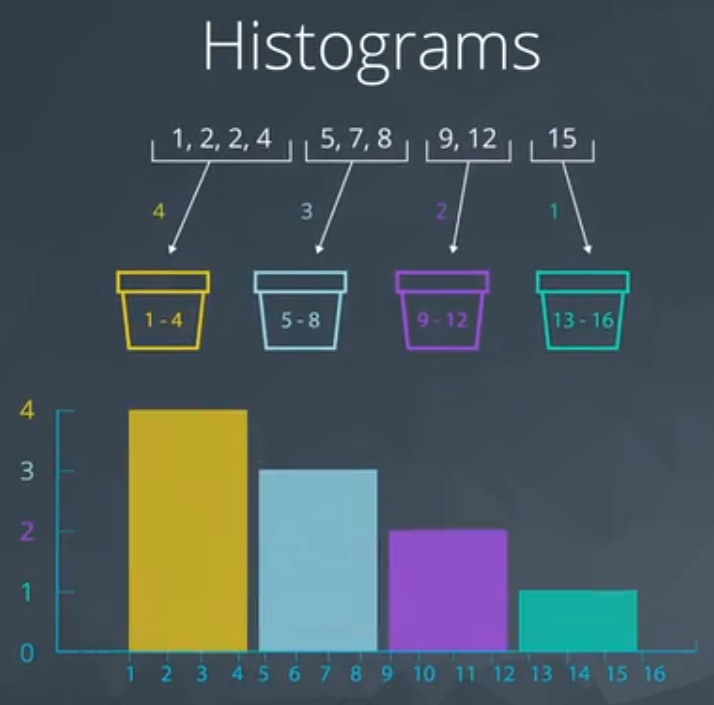
\includegraphics{01-img/c4_l2_01.png}
\caption{}
\end{figure}

This is a way to visualize the quantitative data.

\subsection{Five Number Summary}\label{five-number-summary}

These are the number:

\begin{itemize}
\tightlist
\item
  Maximum;
\item
  Third quartile or Q3 (75\%);
\item
  Second quartile (it is the same of mean) or Q2 (or 50\%);
\item
  First quartile or Q1 (25\%), and;
\item
  Minimum.
\end{itemize}

First step to do is order the values, as you can see in Figure 2 (odd
set of values).

\begin{figure}
\centering
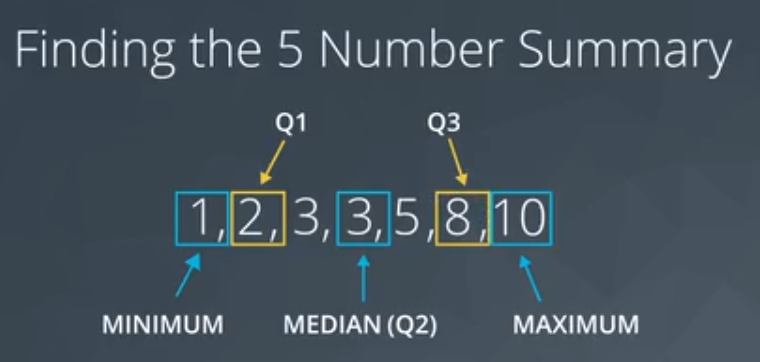
\includegraphics{01-img/c4_l2_02.png}
\caption{}
\end{figure}

As you can see, Q1 and Q3 are the median of the data on either sides of
Q2.

The range is defined as:

\[ \text{Range} = maximum - minimum \tag{1}\]

The Interquartile is define as:

\[ \text{Interquartile} = Q3 - Q1 \tag{2}\]

For a even set of values I need to calculate the ``average'' of two
values.

\begin{figure}
\centering
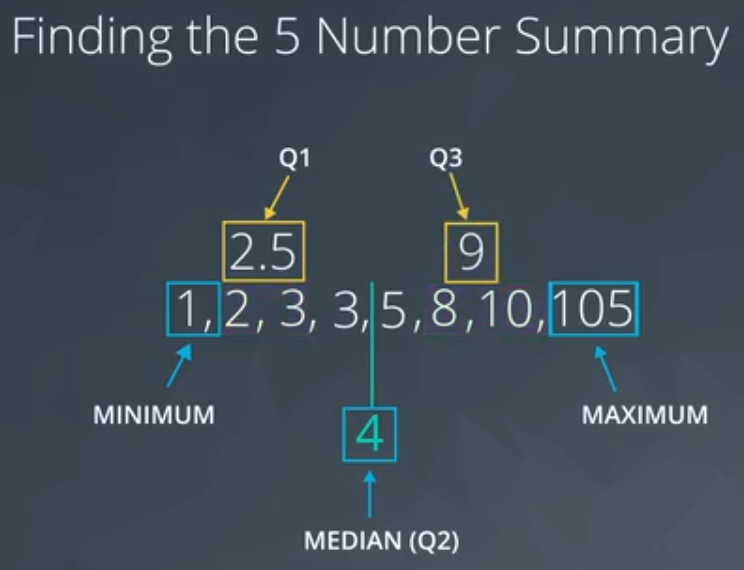
\includegraphics{01-img/c4_l2_03.png}
\caption{}
\end{figure}

\subsubsection{Boxplot}\label{boxplot}

The boxplot graphic is a way to visualize the spread of the data.

\begin{figure}
\centering
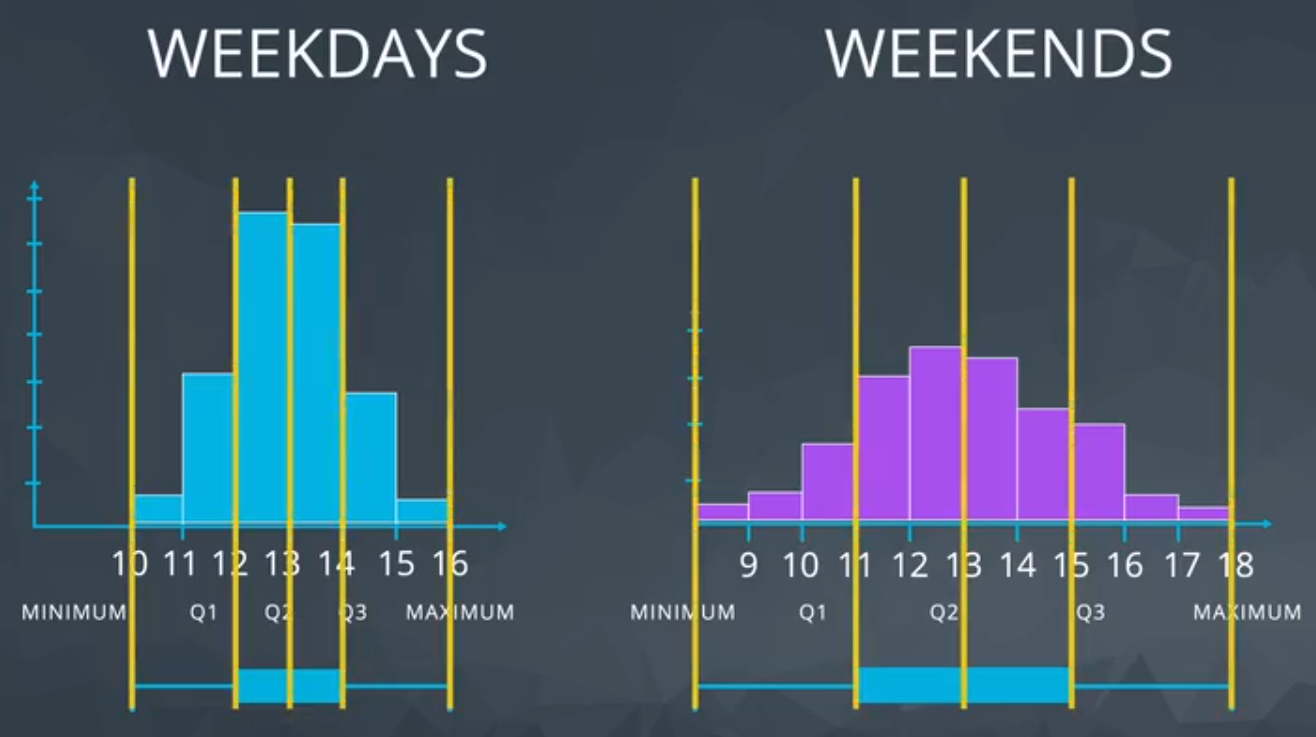
\includegraphics{01-img/c4_l2_04.png}
\caption{}
\end{figure}

It could be useful for quickly comparing the spread of two data sets.

Based on the Figure 4, the graphic on the right shows that in the
weekends the number of dogs varies much more than on weekdays (looking
to the range).

\subsection{Standard Deviation}\label{standard-deviation}

\begin{quote}
Meaning: On average, how much each point varies from the mean of the
points.
\end{quote}

First, I need to define the ``distance'' between mean and each
observation. ``Distance'' could be interpreted as the difference of
these two values. The issue observed in this difference are positive and
negative values. For this reason, the square is used to turn everything
positive (because later I can square root).

\begin{itemize}
\tightlist
\item
  Standard Deviation is frequently used to compare spread of different
  groups.
\item
  Having higher standard deviation is associated with having higher
  risk.
\end{itemize}

\[ \text{Standard Deviation} = \frac{1}{n} \sum_{i = 1}^n (\bar x - x_i)^2 \tag{3}\]

\subsection{Shape}\label{shape}

The shape is related to the histogram form, Figure 5 shows an example.

\begin{figure}
\centering
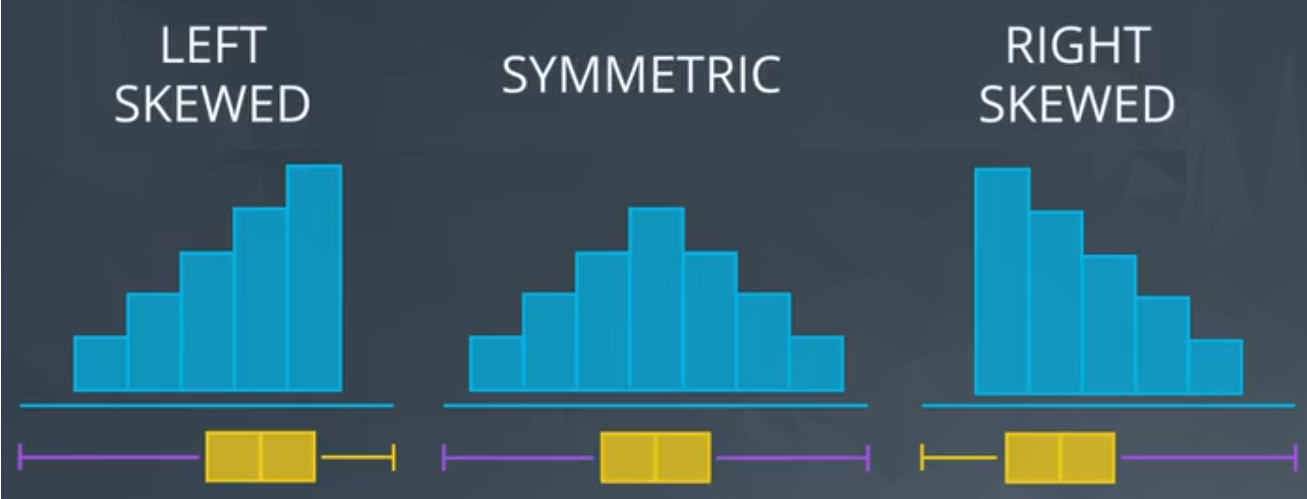
\includegraphics{01-img/c4_l2_05.png}
\caption{}
\end{figure}

\begin{itemize}
\tightlist
\item
  Left Skewed

  \begin{itemize}
  \tightlist
  \item
    is pulled to the ``begining''
  \item
    median stays close to the mode
  \item
    GPA, Age of death, Asset price changes
  \end{itemize}
\item
  Simmetric (example: Normal distribution or bell curve)

  \begin{itemize}
  \tightlist
  \item
    mean = median = mode;
  \item
    Examples: heights, weights, scores, precipitation, etc.
  \end{itemize}
\item
  Right Skewed

  \begin{itemize}
  \tightlist
  \item
    mean is pulled to the tail
  \item
    median stays close to the mode
  \item
    Amount of drug left in your bloodstream over time, distribution of
    wealth, human athletic abilities.
  \end{itemize}
\end{itemize}

\begin{quote}
Side note: If you aren't sure if your data are normally distributed,
there are plots called normal quantile plots and statistical methods
like the Kolmogorov-Smirnov test that are aimed to help you understand
whether or not your data are normally distributed. Implementing this
test is beyond the scope of this class, but can be used as a fun fact.
\end{quote}

\subsection{Outliers}\label{outliers}

\begin{quote}
Data points thah fall very far from the rest of the values in our
dataset.
\end{quote}

The ``very far'' is quite generic and could be interpreted in many
forms. One way to visualize it is plotting a histogram, as you can see
in Figure 6.

\begin{figure}
\centering
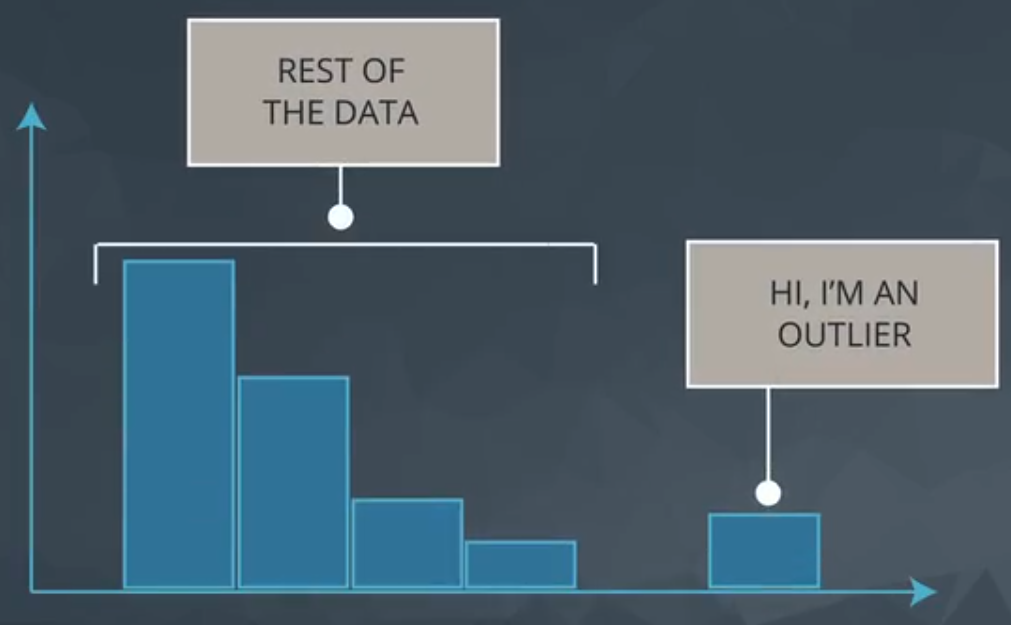
\includegraphics{01-img/c4_l2_06.png}
\caption{}
\end{figure}

\begin{enumerate}
\def\labelenumi{\arabic{enumi}.}
\tightlist
\item
  Note they exist and the impact on summary Statistics
\item
  If typo, remove or fix it.
\item
  Understand why they exist, and the impact on questions we are trying
  to answer
\item
  Reporting the 5 number summary is better than mean and standard
  deviation when outliers are present
\item
  Be careful in reporting know how to ask the right questions
\end{enumerate}

\subsection{Descriptive vs
Inferential}\label{descriptive-vs-inferential}

Descriptive Statistics: Describing Collected Data Inferential
Statistics: Drawing conclusions about a population based on data
collected from sample of individuals from that population.

\section{\texorpdfstring{Admissions Case Study
\texttt{Lesson\ 03}}{Admissions Case Study Lesson 03}}\label{admissions-case-study-lesson-03}

\subsection{Simpson's Paradox}\label{simpsons-paradox}

In this example lesson, you learned about Simpson's Paradox, and you had
the opportunity to apply it to a small example with Sebastian, as well
as work through similar example in Python.

In the lessons ahead, you will be learning a lot by following along with
Sebastian, but it is really important to put these ideas to practice
using data and computing, because that is how you will apply these
skills in a day to day environment as a Data Analyst or Data Scientist.

It is so easy to get caught up in looking at full aggregates of your
data. Hopefully, the examples here serve as a reminder to look at your
data multiple ways.

\subsection{Case Study}\label{case-study}

\section{\texorpdfstring{Probability
\texttt{Lesson\ 04}}{Probability Lesson 04}}\label{probability-lesson-04}

\subsection{Introduction to
Probability}\label{introduction-to-probability}

Do not confound Statistics and Probability.

\begin{itemize}
\tightlist
\item
  Probability: Make preditcions about the future events based on models,
  and;

  \begin{itemize}
  \tightlist
  \item
    Here I want to predict data!
  \end{itemize}
\item
  Statistics: Analyze data from past events to infer what those models
  or causes could be.

  \begin{itemize}
  \tightlist
  \item
    Here I use data to preditc!
  \end{itemize}
\end{itemize}

Figure 1 shows the relation between these two subjects.

\begin{figure}
\centering
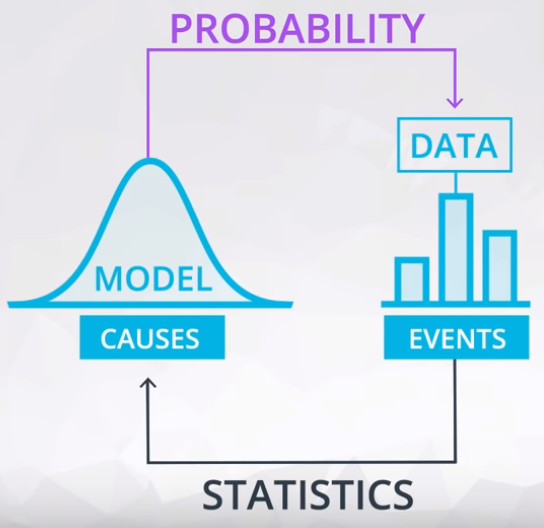
\includegraphics{01-img/c4_l4_01.png}
\caption{}
\end{figure}

\subsubsection{Fair Coin}\label{fair-coin}

The probability notation is based on the 0 to 1 scale, where 0 means
zero percentage and 1 means 100 percentage. The example below is a 50\%.

\[ P(HEADS) = 0.5 \]

To be a fair coin the tail probability it is the same of heads.

\[ P(TAILS) = 0.5 \]

\subsubsection{Loaded Coin}\label{loaded-coin}

Its occurs when the \(P(HEADS)\) is different of \(P(TAILS)\). Bear in
mind, in the equation 1.

\[ P(HEADS) + P(TAILS) = 1 \tag{1}\]

\textbf{Example 1:} \{HEADS, HEADS\} = \(P(H, H)\) for a fair coin.

\(P(H) = P(T) = 0.5\)

To ilustrate this solution, let's draw the Truth Table (Table 1)

Table 1 - Truth Table for a Fair Coin

\begin{longtable}[]{@{}ccc@{}}
\toprule
Flip 1 & Flip 2 & Probability\tabularnewline
\midrule
\endhead
H & H & \$ 0.5 * 0.5 = 0.25 \$\tabularnewline
H & T & \$ 0.5 * 0.5 = 0.25 \$\tabularnewline
T & H & \$ 0.5 * 0.5 = 0.25 \$\tabularnewline
T & T & \$ 0.5 * 0.5 = 0.25 \$\tabularnewline
& & \$ SUM = 1.0 \$\tabularnewline
\bottomrule
\end{longtable}

The probability of P(H, H) is 0.25.

\textbf{Example 2:} \{HEADS, HEADS\} = \(P(H, H)\) for a loaded coin.

\$ P(H) = 0.6 \$ \$ P(T) = 0.4 \$

To ilustrate this solution, let's draw the Truth Table (Table 2)

Table 2 - Truth Table for a Loaded Coin

\begin{longtable}[]{@{}ccc@{}}
\toprule
Flip 1 & Flip 2 & Probability\tabularnewline
\midrule
\endhead
H & H & \$ 0.6 * 0.6 = 0.36 \$\tabularnewline
H & T & \$ 0.6 * 0.4 = 0.24 \$\tabularnewline
T & H & \$ 0.4 * 0.6 = 0.24 \$\tabularnewline
T & T & \$ 0.4 * 0.4 = 0.16 \$\tabularnewline
& & \$ SUM = 1.0 \$\tabularnewline
\bottomrule
\end{longtable}

The probability of P(H, H) is 0.36.

\textbf{Example 3:} Three coins flipped. What is the probability of only
one heads in three coins flipped. Adopting a fair coin (\$ P(H) = 0.5
\$).

\(P_1(Only one H)\)

Table 3 - Truth Table for a Loaded Coin

\begin{longtable}[]{@{}cccccc@{}}
\toprule
Flip 1 & Flip 2 & Flip 3 & Probability & Has only one heads? &
\(P_1\)\tabularnewline
\midrule
\endhead
H & H & H & \$ 0.5 * 0.5 * 0.5 = 0.125 \$ & No & 0\tabularnewline
H & H & T & \$ 0.5 * 0.5 * 0.5 = 0.125 \$ & No & 0\tabularnewline
H & T & H & \$ 0.5 * 0.5 * 0.5 = 0.125 \$ & No & 0\tabularnewline
H & T & T & \$ 0.5 * 0.5 * 0.5 = 0.125 \$ & Yes & 0.125\tabularnewline
T & H & H & \$ 0.5 * 0.5 * 0.5 = 0.125 \$ & No & 0\tabularnewline
T & H & T & \$ 0.5 * 0.5 * 0.5 = 0.125 \$ & Yes & 0.125\tabularnewline
T & T & H & \$ 0.5 * 0.5 * 0.5 = 0.125 \$ & Yes & 0.125\tabularnewline
T & T & T & \$ 0.5 * 0.5 * 0.5 = 0.125 \$ & No & 0\tabularnewline
& & & \$ SUM = 1.0 \$ & \$ SUM = 3 \text{ cases} \$ & \$ SUM = 0.375
\$\tabularnewline
\bottomrule
\end{longtable}

The \$ P\_1 \$ is 0.375.

\textbf{Example 4:} Three coins flipped. What is the probability of only
one heads in three coins flipped. Adopting a loaded coin (\$ P(H) = 0.6
\$).

\(P_2(Only one H)\)

Table 3 - Truth Table for a Loaded Coin

\begin{longtable}[]{@{}cccccc@{}}
\toprule
Flip 1 & Flip 2 & Flip 3 & Probability & Has only one heads? &
\(P_2\)\tabularnewline
\midrule
\endhead
H & H & H & \$ 0.6 * 0.6 * 0.6 = 0.216 \$ & No & 0\tabularnewline
H & H & T & \$ 0.6 * 0.6 * 0.4 = 0.144 \$ & No & 0\tabularnewline
H & T & H & \$ 0.6 * 0.4 * 0.6 = 0.144 \$ & No & 0\tabularnewline
H & T & T & \$ 0.6 * 0.4 * 0.4 = 0.096 \$ & Yes & 0.096\tabularnewline
T & H & H & \$ 0.4 * 0.6 * 0.6 = 0.144 \$ & No & 0\tabularnewline
T & H & T & \$ 0.4 * 0.6 * 0.4 = 0.096 \$ & Yes & 0.096\tabularnewline
T & T & H & \$ 0.4 * 0.4 * 0.6 = 0.096 \$ & Yes & 0.096\tabularnewline
T & T & T & \$ 0.4 * 0.4 * 0.4 = 0.064 \$ & No & 0\tabularnewline
& & & \$ SUM = 1.0 \$ & \$ SUM = 3 \text{ cases} \$ & \$ SUM = 0.288
\$\tabularnewline
\bottomrule
\end{longtable}

The \$ P\_2 \$ is 0.288.

\subsection{Bernoulli Distribution}\label{bernoulli-distribution}

Founded on this introduction, let's generalize this concept using the
Bernoulli Distribution.

\begin{quote}
In probability theory and statistics, the Bernoulli distribution, named
after Swiss mathematician Jacob Bernoulli, is the discrete probability
distribution of a random variable which takes the value 1 with
probability \({\displaystyle p}\) and the value 0 with probability
\({\displaystyle q=1-p,}\) that is, the probability distribution of any
single experiment that asks a yes--no question; the question results in
a boolean-valued outcome, a single bit of information whose value is
success/yes/true/one with probability p and failure/no/false/zero with
probability q. It can be used to represent a (possibly biased) coin toss
where 1 and 0 would represent ``heads'' and ``tails'' (or vice versa),
respectively, and p would be the probability of the coin landing on
heads or tails, respectively. In particular, unfair coins would have
\({\displaystyle p\neq 1/2.}\)
\end{quote}

\begin{quote}
The Bernoulli distribution is a special case of the binomial
distribution where a single trial is conducted (so n would be 1 for such
a binomial distribution). It is also a special case of the two-point
distribution, for which the possible outcomes need not be 0 and 1. --
\href{https://en.wikipedia.org/wiki/Bernoulli_distribution}{Wikipedia}
\end{quote}

Rede more in
\href{http://mathworld.wolfram.com/BernoulliDistribution.html}{wolfram}.

\subsubsection{Summary}\label{summary}

\begin{quote}
Here you learned some fundamental rules of probability. Using notation,
we could say that the outcome of a coin flip could either be T or H for
the event that the coin flips tails or heads, respectively.
\end{quote}

\begin{quote}
Then the following rules are true:
\end{quote}

\begin{itemize}
\item
  Probability of a Event \textgreater{} \[\bold{P(H)} = 0.5\]
\item
  Probability of opposite event \textgreater{}
  \[\bold{1 - P(H) = P(\text{not H})} = 0.5\]
\end{itemize}

\begin{quote}
where \(\bold{\text{not H}}\) is the event of anything other than heads.
Since, there are only two possible outcomes, we have that
\(\bold{P(\text{not H}) = P(T)} = 0.5\). In later concepts, you will see
this with the following notation: \(\bold{\lnot H}\).
\end{quote}

\begin{itemize}
\tightlist
\item
  Probability of composite event
\end{itemize}

\[ P * P * P * \dots * P \]

It is only true because the events are independent of one another, which
means the outcome of one does not affect the outcome of another.

\begin{quote}
\begin{itemize}
\tightlist
\item
  Across multiple coin flips, we have the probability of seeing n heads
  as \(\bold{P(H)^n}\). This is because these events are independent.
\end{itemize}
\end{quote}

\begin{quote}
We can get two generic rules from this:
\end{quote}

\begin{quote}
\begin{enumerate}
\def\labelenumi{\arabic{enumi}.}
\tightlist
\item
  The probability of any event must be between 0 and 1, inclusive.
\end{enumerate}
\end{quote}

\begin{quote}
\begin{enumerate}
\def\labelenumi{\arabic{enumi}.}
\setcounter{enumi}{1}
\tightlist
\item
  The probability of the compliment event is 1 minus the probability of
  an event. That is the probability of all other possible events is 1
  minus the probability an event itself. Therefore, the sum of all
  possible events is equal to 1.
\end{enumerate}
\end{quote}

\begin{quote}
\begin{enumerate}
\def\labelenumi{\arabic{enumi}.}
\setcounter{enumi}{2}
\tightlist
\item
  If our events are independent, then the probability of the string of
  possible events is the product of those events. That is the
  probability of one event AND the next AND the next event, is the
  product of those events.
\end{enumerate}
\end{quote}

\subsubsection{Looking Ahead}\label{looking-ahead}

\begin{quote}
You will be working with the Binomial Distribution, which creates a
function for working with coin flip events like the first events in this
lesson. These events are independent, and the above rules will hold.
from Text: Recap + Next Steps
\end{quote}

\subsection{Conditional Probability}\label{conditional-probability}

Here the first event will affect the second one. Figure 1 shows an
example of it.

\begin{figure}
\centering
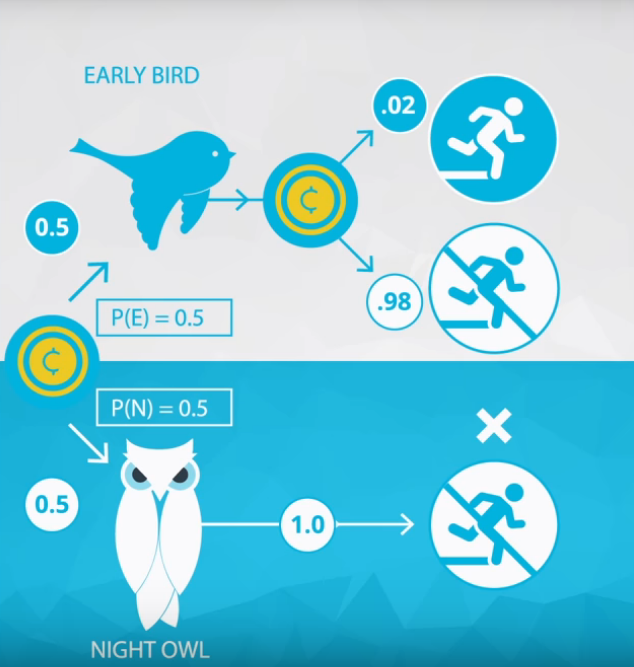
\includegraphics{01-img/c4_l6_01.png}
\caption{Figure 1}
\end{figure}

Figure 1 - Example of conditional probability.

The first event is to determine the bird type, and the second event the
probability to run on the morning. Have in mind, these two birds has
different probability to run on the morning.

\begin{itemize}
\tightlist
\item
  The early bird has 0.02;
\item
  The night owl has 0.00.
\end{itemize}

\subsubsection{Medical Example}\label{medical-example}

Supose a patient with a disease, the probability of this patient has
cancer is 0.9 and to be free cancer is 0.1.

\[P(cancer) = 0.1 \\
  P(\neg \ cancer) = 0.9 \tag{1}\]

To be honest, we do not know if this patient has cancer, so it is
necessary to apply a test. This test is not perfect, it means, there are
a probability to indicates a false positive and a false negative.

For this reason, I introduce the conditional probability.

\[ P(Positive | cancer) = 0.9 \tag{2}\]

\emph{What is the meaning of this notation?}

Given the patient has cancer, the probability of this test indicates
positive is 0.9. Thus, given the patient has cancer and the test
indicates negative is 0.1, as shown in equation (3).

\[ P(Negative | cancer) = 0.1 \tag{3}\]

Analogous to the case of the patient do not has cancer.

\[ P(Positive | \neg \ cancer) = 0.2 \\
   P(Negative | \neg \ cancer) = 0.8 \tag{2} \]

Table 1 shows a representation in a tabular way.

Table 1 - Truth Table for Medical Example

\begin{longtable}[]{@{}ccccccc@{}}
\toprule
\begin{minipage}[b]{0.04\columnwidth}\centering\strut
Disease\strut
\end{minipage} & \begin{minipage}[b]{0.04\columnwidth}\centering\strut
Test\strut
\end{minipage} & \begin{minipage}[b]{0.04\columnwidth}\centering\strut
\(P_{disease}\)\strut
\end{minipage} & \begin{minipage}[b]{0.04\columnwidth}\centering\strut
\(P_{test}\)\strut
\end{minipage} & \begin{minipage}[b]{0.04\columnwidth}\centering\strut
P\strut
\end{minipage} & \begin{minipage}[b]{0.04\columnwidth}\centering\strut
Q1: Test Positive?\strut
\end{minipage} & \begin{minipage}[b]{0.04\columnwidth}\centering\strut
Q1: Answer\strut
\end{minipage}\tabularnewline
\midrule
\endhead
\begin{minipage}[t]{0.04\columnwidth}\centering\strut
No\strut
\end{minipage} & \begin{minipage}[t]{0.04\columnwidth}\centering\strut
Negative\strut
\end{minipage} & \begin{minipage}[t]{0.04\columnwidth}\centering\strut
\(P(\neg \ cancer) = 0.9\)\strut
\end{minipage} & \begin{minipage}[t]{0.04\columnwidth}\centering\strut
\(P(Negative\|\neg \ cancer) = 0.8\)\strut
\end{minipage} & \begin{minipage}[t]{0.04\columnwidth}\centering\strut
0.72\strut
\end{minipage} & \begin{minipage}[t]{0.04\columnwidth}\centering\strut
No\strut
\end{minipage} & \begin{minipage}[t]{0.04\columnwidth}\centering\strut
0\strut
\end{minipage}\tabularnewline
\begin{minipage}[t]{0.04\columnwidth}\centering\strut
No\strut
\end{minipage} & \begin{minipage}[t]{0.04\columnwidth}\centering\strut
Positive\strut
\end{minipage} & \begin{minipage}[t]{0.04\columnwidth}\centering\strut
\(P(\neg \ cancer) = 0.9\)\strut
\end{minipage} & \begin{minipage}[t]{0.04\columnwidth}\centering\strut
\(P(Positive\|\neg \ cancer) = 0.2\)\strut
\end{minipage} & \begin{minipage}[t]{0.04\columnwidth}\centering\strut
0.18\strut
\end{minipage} & \begin{minipage}[t]{0.04\columnwidth}\centering\strut
Yes\strut
\end{minipage} & \begin{minipage}[t]{0.04\columnwidth}\centering\strut
0.18\strut
\end{minipage}\tabularnewline
\begin{minipage}[t]{0.04\columnwidth}\centering\strut
Yes\strut
\end{minipage} & \begin{minipage}[t]{0.04\columnwidth}\centering\strut
Negative\strut
\end{minipage} & \begin{minipage}[t]{0.04\columnwidth}\centering\strut
\(P(cancer) = 0.1\)\strut
\end{minipage} & \begin{minipage}[t]{0.04\columnwidth}\centering\strut
\(P(Negative\| cancer) = 0.1\)\strut
\end{minipage} & \begin{minipage}[t]{0.04\columnwidth}\centering\strut
0.01\strut
\end{minipage} & \begin{minipage}[t]{0.04\columnwidth}\centering\strut
No\strut
\end{minipage} & \begin{minipage}[t]{0.04\columnwidth}\centering\strut
0\strut
\end{minipage}\tabularnewline
\begin{minipage}[t]{0.04\columnwidth}\centering\strut
Yes\strut
\end{minipage} & \begin{minipage}[t]{0.04\columnwidth}\centering\strut
Positive\strut
\end{minipage} & \begin{minipage}[t]{0.04\columnwidth}\centering\strut
\(P(cancer) = 0.1\)\strut
\end{minipage} & \begin{minipage}[t]{0.04\columnwidth}\centering\strut
\(P(Positive\| cancer) = 0.9\)\strut
\end{minipage} & \begin{minipage}[t]{0.04\columnwidth}\centering\strut
0.09\strut
\end{minipage} & \begin{minipage}[t]{0.04\columnwidth}\centering\strut
Yes\strut
\end{minipage} & \begin{minipage}[t]{0.04\columnwidth}\centering\strut
0.09\strut
\end{minipage}\tabularnewline
\begin{minipage}[t]{0.04\columnwidth}\centering\strut
\strut
\end{minipage} & \begin{minipage}[t]{0.04\columnwidth}\centering\strut
\strut
\end{minipage} & \begin{minipage}[t]{0.04\columnwidth}\centering\strut
\strut
\end{minipage} & \begin{minipage}[t]{0.04\columnwidth}\centering\strut
\strut
\end{minipage} & \begin{minipage}[t]{0.04\columnwidth}\centering\strut
\(SUM = 1\)\strut
\end{minipage} & \begin{minipage}[t]{0.04\columnwidth}\centering\strut
\strut
\end{minipage} & \begin{minipage}[t]{0.04\columnwidth}\centering\strut
\(SUM = 0.27\)\strut
\end{minipage}\tabularnewline
\bottomrule
\end{longtable}

\begin{quote}
What is the probability the test is positive?
\end{quote}

\textbf{Q1: 0.27}

\subsubsection*{Coin flip example}\label{coin-flip-example}
\addcontentsline{toc}{subsubsection}{Coin flip example}

Two coins, one fair and other loaded.

\begin{itemize}
\tightlist
\item
  Coin 1: \(P_1(HEADS) = P_1(TAILS) = 0.5\);
\item
  Coin 2: \(P_2(HEADS) = 0.9\) and \(P_2(TAILS) = 0.1\).
\end{itemize}

\begin{figure}
\centering
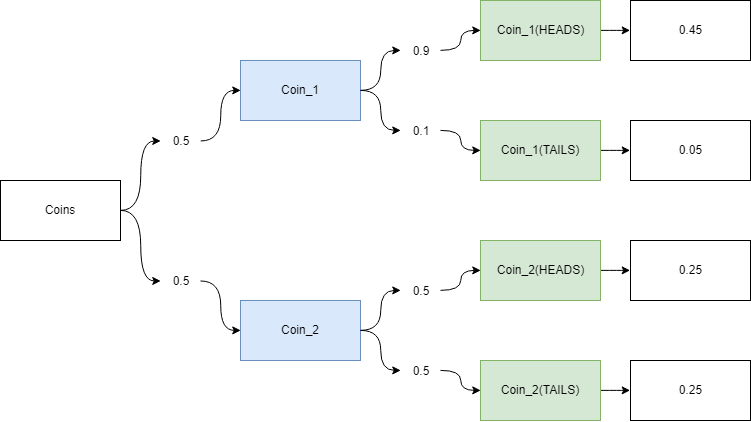
\includegraphics{01-img/c4_l6_02.png}
\caption{Figure 2}
\end{figure}

Figure 2 - Coin Example of conditional probability.

\emph{What is the probability of this sequence HEADS and TAILS?}

\begin{longtable}[]{@{}ccccccccc@{}}
\toprule
\begin{minipage}[b]{0.04\columnwidth}\centering\strut
Coin\strut
\end{minipage} & \begin{minipage}[b]{0.04\columnwidth}\centering\strut
Flip 1\strut
\end{minipage} & \begin{minipage}[b]{0.04\columnwidth}\centering\strut
Flip 2\strut
\end{minipage} & \begin{minipage}[b]{0.04\columnwidth}\centering\strut
\(P_{coin}\)\strut
\end{minipage} & \begin{minipage}[b]{0.04\columnwidth}\centering\strut
\(P_{Flip 1}\)\strut
\end{minipage} & \begin{minipage}[b]{0.04\columnwidth}\centering\strut
\(P_{Flip 2}\)\strut
\end{minipage} & \begin{minipage}[b]{0.04\columnwidth}\centering\strut
P\strut
\end{minipage} & \begin{minipage}[b]{0.04\columnwidth}\centering\strut
Q2: HEADS then TAILS?\strut
\end{minipage} & \begin{minipage}[b]{0.04\columnwidth}\centering\strut
Q2: answer\strut
\end{minipage}\tabularnewline
\midrule
\endhead
\begin{minipage}[t]{0.04\columnwidth}\centering\strut
1\strut
\end{minipage} & \begin{minipage}[t]{0.04\columnwidth}\centering\strut
H\strut
\end{minipage} & \begin{minipage}[t]{0.04\columnwidth}\centering\strut
H\strut
\end{minipage} & \begin{minipage}[t]{0.04\columnwidth}\centering\strut
0.5\strut
\end{minipage} & \begin{minipage}[t]{0.04\columnwidth}\centering\strut
0.9\strut
\end{minipage} & \begin{minipage}[t]{0.04\columnwidth}\centering\strut
0.9\strut
\end{minipage} & \begin{minipage}[t]{0.04\columnwidth}\centering\strut
0.405\strut
\end{minipage} & \begin{minipage}[t]{0.04\columnwidth}\centering\strut
No\strut
\end{minipage} & \begin{minipage}[t]{0.04\columnwidth}\centering\strut
0\strut
\end{minipage}\tabularnewline
\begin{minipage}[t]{0.04\columnwidth}\centering\strut
1\strut
\end{minipage} & \begin{minipage}[t]{0.04\columnwidth}\centering\strut
H\strut
\end{minipage} & \begin{minipage}[t]{0.04\columnwidth}\centering\strut
T\strut
\end{minipage} & \begin{minipage}[t]{0.04\columnwidth}\centering\strut
0.5\strut
\end{minipage} & \begin{minipage}[t]{0.04\columnwidth}\centering\strut
0.9\strut
\end{minipage} & \begin{minipage}[t]{0.04\columnwidth}\centering\strut
0.1\strut
\end{minipage} & \begin{minipage}[t]{0.04\columnwidth}\centering\strut
0.045\strut
\end{minipage} & \begin{minipage}[t]{0.04\columnwidth}\centering\strut
Yes\strut
\end{minipage} & \begin{minipage}[t]{0.04\columnwidth}\centering\strut
0.045\strut
\end{minipage}\tabularnewline
\begin{minipage}[t]{0.04\columnwidth}\centering\strut
1\strut
\end{minipage} & \begin{minipage}[t]{0.04\columnwidth}\centering\strut
T\strut
\end{minipage} & \begin{minipage}[t]{0.04\columnwidth}\centering\strut
H\strut
\end{minipage} & \begin{minipage}[t]{0.04\columnwidth}\centering\strut
0.5\strut
\end{minipage} & \begin{minipage}[t]{0.04\columnwidth}\centering\strut
0.1\strut
\end{minipage} & \begin{minipage}[t]{0.04\columnwidth}\centering\strut
0.9\strut
\end{minipage} & \begin{minipage}[t]{0.04\columnwidth}\centering\strut
0.045\strut
\end{minipage} & \begin{minipage}[t]{0.04\columnwidth}\centering\strut
No\strut
\end{minipage} & \begin{minipage}[t]{0.04\columnwidth}\centering\strut
0\strut
\end{minipage}\tabularnewline
\begin{minipage}[t]{0.04\columnwidth}\centering\strut
1\strut
\end{minipage} & \begin{minipage}[t]{0.04\columnwidth}\centering\strut
T\strut
\end{minipage} & \begin{minipage}[t]{0.04\columnwidth}\centering\strut
T\strut
\end{minipage} & \begin{minipage}[t]{0.04\columnwidth}\centering\strut
0.5\strut
\end{minipage} & \begin{minipage}[t]{0.04\columnwidth}\centering\strut
0.1\strut
\end{minipage} & \begin{minipage}[t]{0.04\columnwidth}\centering\strut
0.1\strut
\end{minipage} & \begin{minipage}[t]{0.04\columnwidth}\centering\strut
0.005\strut
\end{minipage} & \begin{minipage}[t]{0.04\columnwidth}\centering\strut
No\strut
\end{minipage} & \begin{minipage}[t]{0.04\columnwidth}\centering\strut
0\strut
\end{minipage}\tabularnewline
\begin{minipage}[t]{0.04\columnwidth}\centering\strut
2\strut
\end{minipage} & \begin{minipage}[t]{0.04\columnwidth}\centering\strut
H\strut
\end{minipage} & \begin{minipage}[t]{0.04\columnwidth}\centering\strut
H\strut
\end{minipage} & \begin{minipage}[t]{0.04\columnwidth}\centering\strut
0.5\strut
\end{minipage} & \begin{minipage}[t]{0.04\columnwidth}\centering\strut
0.5\strut
\end{minipage} & \begin{minipage}[t]{0.04\columnwidth}\centering\strut
0.5\strut
\end{minipage} & \begin{minipage}[t]{0.04\columnwidth}\centering\strut
0.125\strut
\end{minipage} & \begin{minipage}[t]{0.04\columnwidth}\centering\strut
No\strut
\end{minipage} & \begin{minipage}[t]{0.04\columnwidth}\centering\strut
0\strut
\end{minipage}\tabularnewline
\begin{minipage}[t]{0.04\columnwidth}\centering\strut
2\strut
\end{minipage} & \begin{minipage}[t]{0.04\columnwidth}\centering\strut
H\strut
\end{minipage} & \begin{minipage}[t]{0.04\columnwidth}\centering\strut
T\strut
\end{minipage} & \begin{minipage}[t]{0.04\columnwidth}\centering\strut
0.5\strut
\end{minipage} & \begin{minipage}[t]{0.04\columnwidth}\centering\strut
0.5\strut
\end{minipage} & \begin{minipage}[t]{0.04\columnwidth}\centering\strut
0.5\strut
\end{minipage} & \begin{minipage}[t]{0.04\columnwidth}\centering\strut
0.125\strut
\end{minipage} & \begin{minipage}[t]{0.04\columnwidth}\centering\strut
Yes\strut
\end{minipage} & \begin{minipage}[t]{0.04\columnwidth}\centering\strut
0.125\strut
\end{minipage}\tabularnewline
\begin{minipage}[t]{0.04\columnwidth}\centering\strut
2\strut
\end{minipage} & \begin{minipage}[t]{0.04\columnwidth}\centering\strut
T\strut
\end{minipage} & \begin{minipage}[t]{0.04\columnwidth}\centering\strut
H\strut
\end{minipage} & \begin{minipage}[t]{0.04\columnwidth}\centering\strut
0.5\strut
\end{minipage} & \begin{minipage}[t]{0.04\columnwidth}\centering\strut
0.5\strut
\end{minipage} & \begin{minipage}[t]{0.04\columnwidth}\centering\strut
0.5\strut
\end{minipage} & \begin{minipage}[t]{0.04\columnwidth}\centering\strut
0.125\strut
\end{minipage} & \begin{minipage}[t]{0.04\columnwidth}\centering\strut
No\strut
\end{minipage} & \begin{minipage}[t]{0.04\columnwidth}\centering\strut
0\strut
\end{minipage}\tabularnewline
\begin{minipage}[t]{0.04\columnwidth}\centering\strut
2\strut
\end{minipage} & \begin{minipage}[t]{0.04\columnwidth}\centering\strut
T\strut
\end{minipage} & \begin{minipage}[t]{0.04\columnwidth}\centering\strut
T\strut
\end{minipage} & \begin{minipage}[t]{0.04\columnwidth}\centering\strut
0.5\strut
\end{minipage} & \begin{minipage}[t]{0.04\columnwidth}\centering\strut
0.5\strut
\end{minipage} & \begin{minipage}[t]{0.04\columnwidth}\centering\strut
0.5\strut
\end{minipage} & \begin{minipage}[t]{0.04\columnwidth}\centering\strut
0.125\strut
\end{minipage} & \begin{minipage}[t]{0.04\columnwidth}\centering\strut
No\strut
\end{minipage} & \begin{minipage}[t]{0.04\columnwidth}\centering\strut
0\strut
\end{minipage}\tabularnewline
\begin{minipage}[t]{0.04\columnwidth}\centering\strut
\strut
\end{minipage} & \begin{minipage}[t]{0.04\columnwidth}\centering\strut
\strut
\end{minipage} & \begin{minipage}[t]{0.04\columnwidth}\centering\strut
\strut
\end{minipage} & \begin{minipage}[t]{0.04\columnwidth}\centering\strut
\strut
\end{minipage} & \begin{minipage}[t]{0.04\columnwidth}\centering\strut
\strut
\end{minipage} & \begin{minipage}[t]{0.04\columnwidth}\centering\strut
\strut
\end{minipage} & \begin{minipage}[t]{0.04\columnwidth}\centering\strut
\(SUM = 1\)\strut
\end{minipage} & \begin{minipage}[t]{0.04\columnwidth}\centering\strut
\strut
\end{minipage} & \begin{minipage}[t]{0.04\columnwidth}\centering\strut
\(SUM = 0.170\)\strut
\end{minipage}\tabularnewline
\bottomrule
\end{longtable}

\subsubsection{Summary}\label{summary-1}

\begin{quote}
In this lesson you learned about conditional probability. Often events
are not independent like with coin flips and dice rolling. Instead, the
outcome of one event depends on an earlier event.
\end{quote}

\begin{quote}
For example, the probability of obtaining a positive test result is
dependent on whether or not you have a particular condition. If you have
a condition, it is more likely that a test result is positive. We can
formulate conditional probabilities for any two events in the following
way:
\end{quote}

\begin{quote}
\begin{itemize}
\tightlist
\item
  \(P(A|B) = \frac{P(A\text{ }\cap\text{ }B)}{P(B)}\)
\item
  \(P(A ∩ B)\)
\end{itemize}
\end{quote}

\begin{quote}
In this case, we could have this as:
\end{quote}

\begin{quote}
\[P(positive|disease) = \frac{P(\text{positive }\cap\text{ disease})}{P(disease)}\]
\end{quote}

\begin{quote}
where ∣ represents ``given'' and \(\cap\) represents ``and''. --- Class
notes - Text: Summary
\end{quote}

\section{\texorpdfstring{Binomial Distribution
\texttt{Lesson\ 05}}{Binomial Distribution Lesson 05}}\label{binomial-distribution-lesson-05}

\begin{quote}
In probability theory and statistics, the binomial distribution with
parameters n and p is the discrete probability distribution of the
number of successes in a sequence of n independent experiments, each
asking a yes--no question, and each with its own boolean-valued outcome:
a random variable containing a single bit of information:
success/yes/true/one (with probability p) or failure/no/false/zero (with
probability q = 1 − p). A single success/failure experiment is also
called a Bernoulli trial or Bernoulli experiment and a sequence of
outcomes is called a Bernoulli process; for a single trial, i.e., n = 1,
the binomial distribution is a Bernoulli distribution. The binomial
distribution is the basis for the popular binomial test of statistical
significance.
\href{https://en.wikipedia.org/wiki/Binomial_distribution}{Wikipedia}
\end{quote}

\textbf{Example 1:} 5 coin flips. \(P(\text{two HEADS})\).

\begin{itemize}
\tightlist
\item
  The order of the HEADS do not matter.
\end{itemize}

What's the number of combinations?

\begin{longtable}[]{@{}ccccc@{}}
\toprule
Flip 1 & Flip 2 & Flip 3 & Flip 4 & Flip 5\tabularnewline
\midrule
\endhead
H & ? & ? & ? & ?\tabularnewline
H & H & ? & ? & ?\tabularnewline
5 & 4 & 1 & 1 & 1\tabularnewline
\bottomrule
\end{longtable}

You can place H in 5 places, after place the first H you only have 4
places. For this reason, there are 20 posibilities.

\[ P_1 = 5 * 4 = 20 \]

Bear in mind, the H's are equal and you can swap each one.

\begin{longtable}[]{@{}cc@{}}
\toprule
\(H_1\) & \(H_2\)\tabularnewline
\midrule
\endhead
? & ?\tabularnewline
2 & 1\tabularnewline
\bottomrule
\end{longtable}

So there are two possible H's to insert in the \(H_1\)

\[ P_2 = 2 * 1 = 2 \]

What this \(P_2\) means?

\begin{quote}
You have two equals instances so the \(P_1\) has double entries. The
good part is the \(P_2\) is used to ``fix'' it.
\end{quote}

\[ P = \frac{P_1}{P_2} = \frac{20}{2} = 10 \]

\textbf{Example 2:} 10 coin flips. \(P(\text{four HEADS})\).

\begin{itemize}
\tightlist
\item
  The order of the HEADS do not matter.
\end{itemize}

What's the number of combinations?

\begin{longtable}[]{@{}cccccccccc@{}}
\toprule
Flip 1 & Flip 2 & Flip 3 & Flip 4 & Flip 5 & Flip 6 & Flip 7 & Flip 8 &
Flip 9 & Flip 10\tabularnewline
\midrule
\endhead
H & ? & ? & ? & ? & ? & ? & ? & ? & ?\tabularnewline
H & H & H & T & H & T & T & T & T & T\tabularnewline
10 & 9 & 8 & 1 & 7 & 1 & 1 & 1 & 1 & 1\tabularnewline
\bottomrule
\end{longtable}

You can place H in 10 places, after place the first H you only have 9
places. For this reason, there are (\(10*9*8*7\)) posibilities.

\[ P_1 = 10*9*8*7 = 5,040 \]

Bear in mind, the H's are equal and you can swap each one.

\begin{longtable}[]{@{}cccc@{}}
\toprule
\(H_1\) & \(H_2\) & \(H_3\) & \(H_4\)\tabularnewline
\midrule
\endhead
? & ? & ? & ?\tabularnewline
4 & 3 & 2 & 1\tabularnewline
\bottomrule
\end{longtable}

So there are two possible H's to insert in the \(H_1\)

\[ P_2 = 4 * 3 * 2 * 1 = 24 \]

What this \(P_2\) means?

\begin{quote}
You have two or more equals instances so the \(P_1\) has ``double''
entries. The good part is the \(P_2\) is used to ``fix'' it.
\end{quote}

\[ P = \frac{P_1}{P_2} = \frac{5,040}{24} = 210 \]

\subsection{Equation}\label{equation}

Founded on the examples above, it is possible to write a equation, given
10 flips (\(k\)) and an expected 3 heads (\(n\)).

\[ P = \frac{P_1}{P_2} = \frac{10 * 9 * 8}{\underbrace{3 * 2 * 1}_{3!}}\]

Let's multiply by (\(7 * 6 * 5 * 4 * 3 * 2 * 1\)) or simply by \(7!\).

\[ P = \frac{P_1}{P_2} = \frac{10 * 9 * 8 * 7!}{3! * 7!} = \frac{\overbrace{10!}^{k!}}{\underbrace{3!}_{n!} * \underbrace{7!}_{(k-n)!}} = \frac{k!}{n!(k-n)!} \tag{1}\]

Equation (1) is also noted as:

\[ C_{n,k} = \begin{pmatrix} n \\ k \end{pmatrix} \tag{2}\]

Equation (2) will only calculate the number of combinations. We can
aggregate the probability.

\begin{itemize}
\tightlist
\item
  \(P(H)\): for heads;
\item
  \(P(T)\): for tails;
\end{itemize}

Given the 10 coins flips, the probability for a single instance, no
matter the order:

\emph{Obs.: Do not confound with permutation notation.}

\[ P_{k,n} = P(H)^n * P(T)^{k-n}\]
\[ P_{10,3} = P(H)^3 * P(T)^{7}\tag{3}\]

For a fair coin.

\[ P_{10,3} = 0.5^3 * 0.5^{7} = 0.000976563 \tag{4}\]

The value of \(P(10,3)\) is for a single time, I know there are many
instances where could happen 3 heads, for this reason I use the
combination.

\[ C_{10,3} = \begin{pmatrix} 10 \\ 3 \end{pmatrix} = \frac{10!}{7!*3!} = 120\]

The probability to happen 3 heads in 10 flips coins is:

\[ P(10|3) = C_{10,3} * P_{10,3} = 120 * 0.000976563 = 0.1171875 \]

Expanding this concept to a all around equation:

\[ P(k|n) = \underbrace{C_{k,n}}_{\text{note 1}} * \underbrace{P_{k,n}}_{\text{note 2}} \tag{5}\]

\begin{itemize}
\tightlist
\item
  note 1: Probability to occur the given \emph{combination} (3 heads and
  7 tails) over the all combinations (\(10^2 = 1,024\));
\item
  note 2: Probability based on the coins (heads and tails
  probabilities).
\end{itemize}

\subsubsection{Additional Info}\label{additional-info}

Do not confound Permutation with Combination.

\begin{itemize}
\tightlist
\item
  Combination: When the order does not matter;
\item
  Permutation: When the order is important.
\end{itemize}

Read more in
\href{https://www.mathplanet.com/education/algebra-2/discrete-mathematics-and-probability/permutations-and-combinations}{mathplanet}.

\section{\texorpdfstring{Conditional Probability
\texttt{Lesson\ 06}}{Conditional Probability Lesson 06}}\label{conditional-probability-lesson-06}

Here the first event will affect the second one. Figure 1 shows an
example of it.

\begin{figure}
\centering
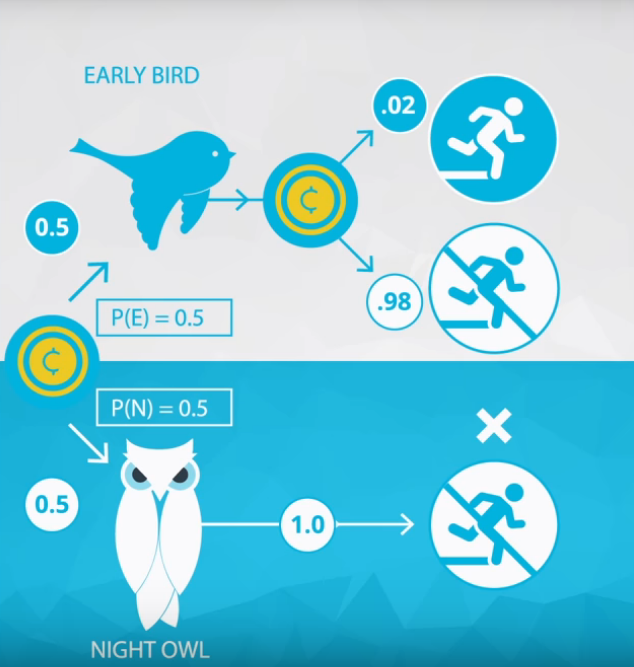
\includegraphics{01-img/c4_l6_01.png}
\caption{Figure 1}
\end{figure}

Figure 1 - Example of conditional probability.

The first event is to determine the bird type, and the second event the
probability to run on the morning. Have in mind, these two birds has
different probability to run on the morning.

\begin{itemize}
\tightlist
\item
  The early bird has 0.02;
\item
  The night owl has 0.00.
\end{itemize}

\subsection{Medical Example}\label{medical-example-1}

Supose a patient with a disease, the probability of this patient has
cancer is 0.9 and to be free cancer is 0.1.

\[P(cancer) = 0.1 \\
  P(\neg \ cancer) = 0.9 \tag{1}\]

To be honest, we do not know if this patient has cancer, so it is
necessary to apply a test. This test is not perfect, it means, there are
a probability to indicates a false positive and a false negative.

For this reason, I introduce the conditional probability.

\[ P(Positive | cancer) = 0.9 \tag{2}\]

\emph{What is the meaning of this notation?}

Given the patient has cancer, the probability of this test indicates
positive is 0.9. Thus, given the patient has cancer and the test
indicates negative is 0.1, as shown in equation (3).

\[ P(Negative | cancer) = 0.1 \tag{3}\]

Analogous to the case of the patient do not has cancer.

\[ P(Positive | \neg \ cancer) = 0.2 \\
   P(Negative | \neg \ cancer) = 0.8 \tag{2} \]

Table 1 shows a representation in a tabular way.

Table 1 - Truth Table for Medical Example

\begin{longtable}[]{@{}ccccccc@{}}
\toprule
\begin{minipage}[b]{0.04\columnwidth}\centering\strut
Disease\strut
\end{minipage} & \begin{minipage}[b]{0.04\columnwidth}\centering\strut
Test\strut
\end{minipage} & \begin{minipage}[b]{0.04\columnwidth}\centering\strut
\(P_{disease}\)\strut
\end{minipage} & \begin{minipage}[b]{0.04\columnwidth}\centering\strut
\(P_{test}\)\strut
\end{minipage} & \begin{minipage}[b]{0.04\columnwidth}\centering\strut
P\strut
\end{minipage} & \begin{minipage}[b]{0.04\columnwidth}\centering\strut
Q1: Test Positive?\strut
\end{minipage} & \begin{minipage}[b]{0.04\columnwidth}\centering\strut
Q1: Answer\strut
\end{minipage}\tabularnewline
\midrule
\endhead
\begin{minipage}[t]{0.04\columnwidth}\centering\strut
No\strut
\end{minipage} & \begin{minipage}[t]{0.04\columnwidth}\centering\strut
Negative\strut
\end{minipage} & \begin{minipage}[t]{0.04\columnwidth}\centering\strut
\(P(\neg \ cancer) = 0.9\)\strut
\end{minipage} & \begin{minipage}[t]{0.04\columnwidth}\centering\strut
\(P(Negative\|\neg \ cancer) = 0.8\)\strut
\end{minipage} & \begin{minipage}[t]{0.04\columnwidth}\centering\strut
0.72\strut
\end{minipage} & \begin{minipage}[t]{0.04\columnwidth}\centering\strut
No\strut
\end{minipage} & \begin{minipage}[t]{0.04\columnwidth}\centering\strut
0\strut
\end{minipage}\tabularnewline
\begin{minipage}[t]{0.04\columnwidth}\centering\strut
No\strut
\end{minipage} & \begin{minipage}[t]{0.04\columnwidth}\centering\strut
Positive\strut
\end{minipage} & \begin{minipage}[t]{0.04\columnwidth}\centering\strut
\(P(\neg \ cancer) = 0.9\)\strut
\end{minipage} & \begin{minipage}[t]{0.04\columnwidth}\centering\strut
\(P(Positive\|\neg \ cancer) = 0.2\)\strut
\end{minipage} & \begin{minipage}[t]{0.04\columnwidth}\centering\strut
0.18\strut
\end{minipage} & \begin{minipage}[t]{0.04\columnwidth}\centering\strut
Yes\strut
\end{minipage} & \begin{minipage}[t]{0.04\columnwidth}\centering\strut
0.18\strut
\end{minipage}\tabularnewline
\begin{minipage}[t]{0.04\columnwidth}\centering\strut
Yes\strut
\end{minipage} & \begin{minipage}[t]{0.04\columnwidth}\centering\strut
Negative\strut
\end{minipage} & \begin{minipage}[t]{0.04\columnwidth}\centering\strut
\(P(cancer) = 0.1\)\strut
\end{minipage} & \begin{minipage}[t]{0.04\columnwidth}\centering\strut
\(P(Negative\| cancer) = 0.1\)\strut
\end{minipage} & \begin{minipage}[t]{0.04\columnwidth}\centering\strut
0.01\strut
\end{minipage} & \begin{minipage}[t]{0.04\columnwidth}\centering\strut
No\strut
\end{minipage} & \begin{minipage}[t]{0.04\columnwidth}\centering\strut
0\strut
\end{minipage}\tabularnewline
\begin{minipage}[t]{0.04\columnwidth}\centering\strut
Yes\strut
\end{minipage} & \begin{minipage}[t]{0.04\columnwidth}\centering\strut
Positive\strut
\end{minipage} & \begin{minipage}[t]{0.04\columnwidth}\centering\strut
\(P(cancer) = 0.1\)\strut
\end{minipage} & \begin{minipage}[t]{0.04\columnwidth}\centering\strut
\(P(Positive\| cancer) = 0.9\)\strut
\end{minipage} & \begin{minipage}[t]{0.04\columnwidth}\centering\strut
0.09\strut
\end{minipage} & \begin{minipage}[t]{0.04\columnwidth}\centering\strut
Yes\strut
\end{minipage} & \begin{minipage}[t]{0.04\columnwidth}\centering\strut
0.09\strut
\end{minipage}\tabularnewline
\begin{minipage}[t]{0.04\columnwidth}\centering\strut
\strut
\end{minipage} & \begin{minipage}[t]{0.04\columnwidth}\centering\strut
\strut
\end{minipage} & \begin{minipage}[t]{0.04\columnwidth}\centering\strut
\strut
\end{minipage} & \begin{minipage}[t]{0.04\columnwidth}\centering\strut
\strut
\end{minipage} & \begin{minipage}[t]{0.04\columnwidth}\centering\strut
\(\sum = 1\)\strut
\end{minipage} & \begin{minipage}[t]{0.04\columnwidth}\centering\strut
\strut
\end{minipage} & \begin{minipage}[t]{0.04\columnwidth}\centering\strut
\(\sum = 0.27\)\strut
\end{minipage}\tabularnewline
\bottomrule
\end{longtable}

\begin{quote}
What is the probability the test is positive?
\end{quote}

\textbf{Q1: 0.27}

\subsubsection{Coin flip example}\label{coin-flip-example-1}

Two coins, one fair and other loaded.

\begin{itemize}
\tightlist
\item
  Coin 1: \(P_1(HEADS) = P_1(TAILS) = 0.5\);
\item
  Coin 2: \(P_2(HEADS) = 0.9\) and \(P_2(TAILS) = 0.1\).
\end{itemize}

\begin{figure}
\centering
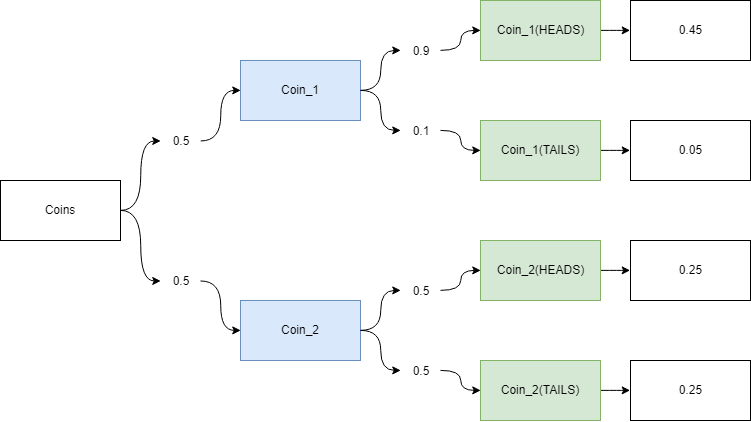
\includegraphics{01-img/c4_l6_02.png}
\caption{Figure 2}
\end{figure}

Figure 2 - Coin Example of conditional probability.

\emph{What is the probability of this sequence HEADS and TAILS?}

\begin{longtable}[]{@{}ccccccccc@{}}
\toprule
\begin{minipage}[b]{0.04\columnwidth}\centering\strut
Coin\strut
\end{minipage} & \begin{minipage}[b]{0.04\columnwidth}\centering\strut
Flip 1\strut
\end{minipage} & \begin{minipage}[b]{0.04\columnwidth}\centering\strut
Flip 2\strut
\end{minipage} & \begin{minipage}[b]{0.04\columnwidth}\centering\strut
\(P_{coin}\)\strut
\end{minipage} & \begin{minipage}[b]{0.04\columnwidth}\centering\strut
\(P_{Flip 1}\)\strut
\end{minipage} & \begin{minipage}[b]{0.04\columnwidth}\centering\strut
\(P_{Flip 2}\)\strut
\end{minipage} & \begin{minipage}[b]{0.04\columnwidth}\centering\strut
P\strut
\end{minipage} & \begin{minipage}[b]{0.04\columnwidth}\centering\strut
Q2: HEADS then TAILS?\strut
\end{minipage} & \begin{minipage}[b]{0.04\columnwidth}\centering\strut
Q2: answer\strut
\end{minipage}\tabularnewline
\midrule
\endhead
\begin{minipage}[t]{0.04\columnwidth}\centering\strut
1\strut
\end{minipage} & \begin{minipage}[t]{0.04\columnwidth}\centering\strut
H\strut
\end{minipage} & \begin{minipage}[t]{0.04\columnwidth}\centering\strut
H\strut
\end{minipage} & \begin{minipage}[t]{0.04\columnwidth}\centering\strut
0.5\strut
\end{minipage} & \begin{minipage}[t]{0.04\columnwidth}\centering\strut
0.9\strut
\end{minipage} & \begin{minipage}[t]{0.04\columnwidth}\centering\strut
0.9\strut
\end{minipage} & \begin{minipage}[t]{0.04\columnwidth}\centering\strut
0.405\strut
\end{minipage} & \begin{minipage}[t]{0.04\columnwidth}\centering\strut
No\strut
\end{minipage} & \begin{minipage}[t]{0.04\columnwidth}\centering\strut
0\strut
\end{minipage}\tabularnewline
\begin{minipage}[t]{0.04\columnwidth}\centering\strut
1\strut
\end{minipage} & \begin{minipage}[t]{0.04\columnwidth}\centering\strut
H\strut
\end{minipage} & \begin{minipage}[t]{0.04\columnwidth}\centering\strut
T\strut
\end{minipage} & \begin{minipage}[t]{0.04\columnwidth}\centering\strut
0.5\strut
\end{minipage} & \begin{minipage}[t]{0.04\columnwidth}\centering\strut
0.9\strut
\end{minipage} & \begin{minipage}[t]{0.04\columnwidth}\centering\strut
0.1\strut
\end{minipage} & \begin{minipage}[t]{0.04\columnwidth}\centering\strut
0.045\strut
\end{minipage} & \begin{minipage}[t]{0.04\columnwidth}\centering\strut
Yes\strut
\end{minipage} & \begin{minipage}[t]{0.04\columnwidth}\centering\strut
0.045\strut
\end{minipage}\tabularnewline
\begin{minipage}[t]{0.04\columnwidth}\centering\strut
1\strut
\end{minipage} & \begin{minipage}[t]{0.04\columnwidth}\centering\strut
T\strut
\end{minipage} & \begin{minipage}[t]{0.04\columnwidth}\centering\strut
H\strut
\end{minipage} & \begin{minipage}[t]{0.04\columnwidth}\centering\strut
0.5\strut
\end{minipage} & \begin{minipage}[t]{0.04\columnwidth}\centering\strut
0.1\strut
\end{minipage} & \begin{minipage}[t]{0.04\columnwidth}\centering\strut
0.9\strut
\end{minipage} & \begin{minipage}[t]{0.04\columnwidth}\centering\strut
0.045\strut
\end{minipage} & \begin{minipage}[t]{0.04\columnwidth}\centering\strut
No\strut
\end{minipage} & \begin{minipage}[t]{0.04\columnwidth}\centering\strut
0\strut
\end{minipage}\tabularnewline
\begin{minipage}[t]{0.04\columnwidth}\centering\strut
1\strut
\end{minipage} & \begin{minipage}[t]{0.04\columnwidth}\centering\strut
T\strut
\end{minipage} & \begin{minipage}[t]{0.04\columnwidth}\centering\strut
T\strut
\end{minipage} & \begin{minipage}[t]{0.04\columnwidth}\centering\strut
0.5\strut
\end{minipage} & \begin{minipage}[t]{0.04\columnwidth}\centering\strut
0.1\strut
\end{minipage} & \begin{minipage}[t]{0.04\columnwidth}\centering\strut
0.1\strut
\end{minipage} & \begin{minipage}[t]{0.04\columnwidth}\centering\strut
0.005\strut
\end{minipage} & \begin{minipage}[t]{0.04\columnwidth}\centering\strut
No\strut
\end{minipage} & \begin{minipage}[t]{0.04\columnwidth}\centering\strut
0\strut
\end{minipage}\tabularnewline
\begin{minipage}[t]{0.04\columnwidth}\centering\strut
2\strut
\end{minipage} & \begin{minipage}[t]{0.04\columnwidth}\centering\strut
H\strut
\end{minipage} & \begin{minipage}[t]{0.04\columnwidth}\centering\strut
H\strut
\end{minipage} & \begin{minipage}[t]{0.04\columnwidth}\centering\strut
0.5\strut
\end{minipage} & \begin{minipage}[t]{0.04\columnwidth}\centering\strut
0.5\strut
\end{minipage} & \begin{minipage}[t]{0.04\columnwidth}\centering\strut
0.5\strut
\end{minipage} & \begin{minipage}[t]{0.04\columnwidth}\centering\strut
0.125\strut
\end{minipage} & \begin{minipage}[t]{0.04\columnwidth}\centering\strut
No\strut
\end{minipage} & \begin{minipage}[t]{0.04\columnwidth}\centering\strut
0\strut
\end{minipage}\tabularnewline
\begin{minipage}[t]{0.04\columnwidth}\centering\strut
2\strut
\end{minipage} & \begin{minipage}[t]{0.04\columnwidth}\centering\strut
H\strut
\end{minipage} & \begin{minipage}[t]{0.04\columnwidth}\centering\strut
T\strut
\end{minipage} & \begin{minipage}[t]{0.04\columnwidth}\centering\strut
0.5\strut
\end{minipage} & \begin{minipage}[t]{0.04\columnwidth}\centering\strut
0.5\strut
\end{minipage} & \begin{minipage}[t]{0.04\columnwidth}\centering\strut
0.5\strut
\end{minipage} & \begin{minipage}[t]{0.04\columnwidth}\centering\strut
0.125\strut
\end{minipage} & \begin{minipage}[t]{0.04\columnwidth}\centering\strut
Yes\strut
\end{minipage} & \begin{minipage}[t]{0.04\columnwidth}\centering\strut
0.125\strut
\end{minipage}\tabularnewline
\begin{minipage}[t]{0.04\columnwidth}\centering\strut
2\strut
\end{minipage} & \begin{minipage}[t]{0.04\columnwidth}\centering\strut
T\strut
\end{minipage} & \begin{minipage}[t]{0.04\columnwidth}\centering\strut
H\strut
\end{minipage} & \begin{minipage}[t]{0.04\columnwidth}\centering\strut
0.5\strut
\end{minipage} & \begin{minipage}[t]{0.04\columnwidth}\centering\strut
0.5\strut
\end{minipage} & \begin{minipage}[t]{0.04\columnwidth}\centering\strut
0.5\strut
\end{minipage} & \begin{minipage}[t]{0.04\columnwidth}\centering\strut
0.125\strut
\end{minipage} & \begin{minipage}[t]{0.04\columnwidth}\centering\strut
No\strut
\end{minipage} & \begin{minipage}[t]{0.04\columnwidth}\centering\strut
0\strut
\end{minipage}\tabularnewline
\begin{minipage}[t]{0.04\columnwidth}\centering\strut
2\strut
\end{minipage} & \begin{minipage}[t]{0.04\columnwidth}\centering\strut
T\strut
\end{minipage} & \begin{minipage}[t]{0.04\columnwidth}\centering\strut
T\strut
\end{minipage} & \begin{minipage}[t]{0.04\columnwidth}\centering\strut
0.5\strut
\end{minipage} & \begin{minipage}[t]{0.04\columnwidth}\centering\strut
0.5\strut
\end{minipage} & \begin{minipage}[t]{0.04\columnwidth}\centering\strut
0.5\strut
\end{minipage} & \begin{minipage}[t]{0.04\columnwidth}\centering\strut
0.125\strut
\end{minipage} & \begin{minipage}[t]{0.04\columnwidth}\centering\strut
No\strut
\end{minipage} & \begin{minipage}[t]{0.04\columnwidth}\centering\strut
0\strut
\end{minipage}\tabularnewline
\begin{minipage}[t]{0.04\columnwidth}\centering\strut
\strut
\end{minipage} & \begin{minipage}[t]{0.04\columnwidth}\centering\strut
\strut
\end{minipage} & \begin{minipage}[t]{0.04\columnwidth}\centering\strut
\strut
\end{minipage} & \begin{minipage}[t]{0.04\columnwidth}\centering\strut
\strut
\end{minipage} & \begin{minipage}[t]{0.04\columnwidth}\centering\strut
\strut
\end{minipage} & \begin{minipage}[t]{0.04\columnwidth}\centering\strut
\strut
\end{minipage} & \begin{minipage}[t]{0.04\columnwidth}\centering\strut
\(\sum = 1\)\strut
\end{minipage} & \begin{minipage}[t]{0.04\columnwidth}\centering\strut
\strut
\end{minipage} & \begin{minipage}[t]{0.04\columnwidth}\centering\strut
\(\sum = 0.170\)\strut
\end{minipage}\tabularnewline
\bottomrule
\end{longtable}

\subsubsection{Summary}\label{summary-2}

\begin{quote}
In this lesson you learned about conditional probability. Often events
are not independent like with coin flips and dice rolling. Instead, the
outcome of one event depends on an earlier event.
\end{quote}

\begin{quote}
For example, the probability of obtaining a positive test result is
dependent on whether or not you have a particular condition. If you have
a condition, it is more likely that a test result is positive. We can
formulate conditional probabilities for any two events in the following
way:
\end{quote}

\begin{quote}
\begin{itemize}
\tightlist
\item
  \(P(A|B) = \frac{P(A\text{ }\cap\text{ }B)}{P(B)}\)
\item
  \(P(A ∩ B)\)
\end{itemize}
\end{quote}

\begin{quote}
In this case, we could have this as:
\end{quote}

\begin{quote}
\[P(positive|disease) = \frac{P(\text{positive }\cap\text{ disease})}{P(disease)}\]
\end{quote}

\begin{quote}
where ∣ represents ``given'' and \(\cap\) represents ``and''. --- Class
notes - Text: Summary
\end{quote}

\section{\texorpdfstring{Bayes Rule
\texttt{Lesson\ 07}}{Bayes Rule Lesson 07}}\label{bayes-rule-lesson-07}

The person who writes down this theorem.

\begin{quote}
Thomas Bayes (/beɪz/; c. 1701 -- 7 April 1761) was an English
statistician, philosopher and Presbyterian minister who is known for
formulating a specific case of the theorem that bears his name: Bayes'
theorem. Bayes never published what would become his most famous
accomplishment; his notes were edited and published after his death by
Richard Price. ---
\href{https://en.wikipedia.org/wiki/Thomas_Bayes}{Wikipedia - Thomas
Bayes}
\end{quote}

\subsection{Cancer Example}\label{cancer-example}

The probability to a person has cancer is 1\% and the probability to the
test gives positive is 90\%. If a person do not has cancer the
probability of the test gives negative is 90\%.

\emph{What is the probability of a given positive test the person has
cancer?}

\begin{longtable}[]{@{}ccccccc@{}}
\toprule
Disease & Test & \(P_{disease}\) & \(P_{test}\) & P & Q1: Test positive?
& Q1: answer\tabularnewline
\midrule
\endhead
No & Negative & 0.99 & 0.90 & 0.891 & No & 0\tabularnewline
No & Positive & 0.99 & 0.10 & 0.099 & Yes & 0.099\tabularnewline
Yes & Negative & 0.01 & 0.10 & 0.001 & No & 0\tabularnewline
Yes & Positive & 0.01 & 0.90 & 0.009 & Yes & 0.009\tabularnewline
& & & & & & SUM = 0.108\tabularnewline
\bottomrule
\end{longtable}

Bear in mind, the probability of a false positive is 0.099, which is 11
times bigger than the a truth valeu of 0.009.

Figure 1 ilustrate this situation.

\begin{figure}
\centering
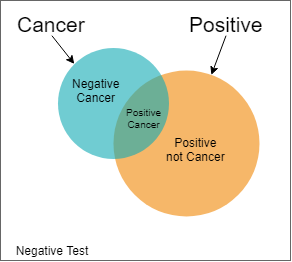
\includegraphics{01-img/c4_l7_01.png}
\caption{}
\end{figure}

Given the test is positive, the probability of this person has cancer
is:

\[ P(C\|Positive) = \frac{P(C,Positive)}{P(C,Positive) + P(\neg \ C,Positive)} = \frac{0.009}{0.009 + 0.099} = 0.08333\]

\subsection{Bayes Rule}\label{bayes-rule}

From the example above, I can point out some definitions:

\textbf{Prior:}

This is a information before the test.

\[ P(C) = 0.01 \\ P(\neg C) = 0.99 \tag{1}\]

\textbf{Joint:}

Now, I will apply the test for a given positive result.

\[ P(C,Positive) = P(C) * \underbrace{P(Positive\|C)}_{Sensibility} \\
   P(\neg C,Positive) = P(\neg \ C) * \underbrace{P(Positive\| \neg \ C)}_{Sensibility} \tag{2} \]

For a negative result.

\[ P(C,Negative) = P(C) * \underbrace{P(Negative\|C)}_{Specitivity} \\
      P(\neg \ C,Negative) = P(\neg \ C) * \underbrace{P(Negative\| \neg \ C)}_{Specitivity} \tag{3}\]

\textbf{Normalization:}

This is performed for each result (Positive and Negative).

\[ P(Positive) = P(C,Positive) + P(\neg \ C,Positive) \tag{4}\]

\textbf{Posterior:}

Divide the \(P(C,Positive)\) and \(P(\neg C,Positive)\) by
\(P(Positive)\).

\[P(C|Positive) = \frac{P(C,Positive)}{P(Positive)} \tag{5}\]

\[P(\neg C|Positive) = \frac{P(\neg C,Positive)}{P(Positive)} \tag{6}\]

Finally, the Bayes equation could be generalized as:

\[P(A|B) = \frac{P(A) * P(B|A)}{P(B)} \tag{7}\]

\section{\texorpdfstring{Python Probability Practice
\texttt{Lesson\ 08}}{Python Probability Practice Lesson 08}}\label{python-probability-practice-lesson-08}

Some methods interesting to take notes.

\subsubsection{\texorpdfstring{\texttt{.random.randint()}}{.random.randint()}}\label{random.randint}

Generates a random value.

\begin{Shaded}
\begin{Highlighting}[]
\KeywordTok{np.random.randint}\NormalTok{(}\DecValTok{0}\NormalTok{, }\DecValTok{2}\NormalTok{, }\DataTypeTok{size=}\DecValTok{10000}\NormalTok{)}
\end{Highlighting}
\end{Shaded}

In the example above, the line code will generate a sample of 10,000
number from 0 to 1 (the 2 is not inclusive).

\subsubsection{\texorpdfstring{\texttt{.random.choice()}}{.random.choice()}}\label{random.choice}

Generates a radom value with different loads.

\begin{Shaded}
\begin{Highlighting}[]
\KeywordTok{np.random.choice}\NormalTok{([}\DecValTok{0}\NormalTok{, }\DecValTok{1}\NormalTok{], }\DataTypeTok{size=}\DecValTok{10000}\NormalTok{, }\DataTypeTok{p=}\NormalTok{[}\FloatTok{0.8}\NormalTok{, }\FloatTok{0.2}\NormalTok{])}\ErrorTok{)}
\end{Highlighting}
\end{Shaded}

In the example the loads are 0.8 and 0.2.

\subsubsection{\texorpdfstring{\texttt{random.binomial()}}{random.binomial()}}\label{random.binomial}

This method is an other way to simulate a coin flip.

\begin{Shaded}
\begin{Highlighting}[]
\KeywordTok{np.random.binomial}\NormalTok{(}\DecValTok{10}\NormalTok{, }\FloatTok{0.5}\NormalTok{, }\DecValTok{1000000}\NormalTok{)}
\end{Highlighting}
\end{Shaded}

The example above will flip 10 coins (with a fair rate due to the 0.5),
with a sample of 1 million.

The result of this methods is a ``aggregation'' of the success events,
which means the output varies from 0 to 10.

\section{\texorpdfstring{Normal Distribution Theory
\texttt{Lesson\ 09}}{Normal Distribution Theory Lesson 09}}\label{normal-distribution-theory-lesson-09}

Comparison between a simple probability, binomial distribution, and
normal distribution.

\begin{longtable}[]{@{}cc@{}}
\toprule
Type & Quantity\tabularnewline
\midrule
\endhead
Bernoulli & 1\tabularnewline
Binomial & 10\tabularnewline
Normal & 1000\tabularnewline
\bottomrule
\end{longtable}

Along this chapter I have seen the evolution from the simple probability
(Bernoulli), to a Binomial, and finally a Normal distribution.

The difference is the size of the ``sample''.

\subsection{Equations}\label{equations}

\begin{itemize}
\tightlist
\item
  Bernoulli
\end{itemize}

\[ P(HEADS) = P(HEADS)^n \tag{1}\]

\begin{itemize}
\tightlist
\item
  Binomial
\end{itemize}

\[P(n,k) = \frac{n!}{(n-k)!k!} p^k * (1-p)^{n-k} \tag{2}\]

\begin{itemize}
\tightlist
\item
  Normal (or Gaussian or Gauss or Laplace--Gauss) distribution
\end{itemize}

\[N(x;\mu,\sigma^2) = \frac{1}{\sqrt{2\pi\sigma^2}}\exp^{-\frac{1}{2} \frac{(x-\mu)^2}{\sigma^2}} \tag{3}\]

\(\mu\): mean; \(\sigma^2\): variance.

\section{\texorpdfstring{Sampling distributions and Central Limit
Theorem
\texttt{Lesson\ 10}}{Sampling distributions and Central Limit Theorem Lesson 10}}\label{sampling-distributions-and-central-limit-theorem-lesson-10}

Recap of Inferential Statistics.

\subsubsection{Inferential Statistics}\label{inferential-statistics}

\begin{quote}
In order to assure you are comfortable with the ideas surrounding
inferential statistics. The next 4 concepts are aimed at the difference
between Descriptive and Inferential Statistics. Actually applying
inferential statistics techniques to data will be taught in later
lessons.
\end{quote}

\subsubsection{Probability to
Statistics}\label{probability-to-statistics}

\begin{quote}
This begins a set of lessons that will be more data oriented in the way
that you are applying ideas, and less probability oriented.
\end{quote}

\begin{quote}
Often we use statistics to verify conclusions of probability through
simulation. Therefore, simulation (similar to the python lesson you
completed earlier) will be a large part of the way we show mathematical
ideas moving forward.
\end{quote}

\paragraph{Solutions}\label{solutions}

\begin{quote}
It is in your best interest to work through the solution notebooks on
your own before looking at the solutions available for this course.
However, if you get stuck or would like to double check your solutions,
notice all of the solutions and data are available in the resources tab
of this course. This is true for all of the following lessons as well.
--- Class notes
\end{quote}

\subsubsection{Comparison Descriptive and Inferential
Statistics}\label{comparison-descriptive-and-inferential-statistics}

\begin{quote}
In this section, we learned about how Inferential Statistics differs
from Descriptive Statistics.
\end{quote}

\begin{quote}
\begin{itemize}
\tightlist
\item
  \texttt{Descriptive\ statistics} is about describing our collected
  data using the measures discussed throughout this lesson: measures of
  center, measures of spread, shape of our distribution, and outliers.
  We can also use plots of our data to gain a better understanding.
\end{itemize}
\end{quote}

\begin{quote}
\begin{itemize}
\tightlist
\item
  \texttt{Inferential\ Statistics} is about using our collected data to
  draw conclusions to a larger population. Performing inferential
  statistics well requires that we take a sample that accurately
  represents our population of interest.
\end{itemize}
\end{quote}

\begin{quote}
A common way to collect data is via a survey. However, surveys may be
extremely biased depending on the types of questions that are asked, and
the way the questions are asked. This is a topic you should think about
when tackling the the first project.
\end{quote}

\begin{quote}
We looked at specific examples that allowed us to identify the
\end{quote}

\begin{quote}
\begin{itemize}
\tightlist
\item
  Population - our entire group of interest.
\item
  Parameter - numeric summary about a population
\item
  Sample - subset of the population
\item
  Statistic numeric summary about a sample
\end{itemize}
\end{quote}

\subsection{Sampling distribution}\label{sampling-distribution}

\begin{quote}
A sampling distribution is the distribution of a statistic. Here we
looked the distribution of the proportion for samples of 5 students.
This is key to the ideas covered not only in this lesson, but in future
lessons.
\end{quote}

\subsection{Notation}\label{notation}

\begin{figure}
\centering
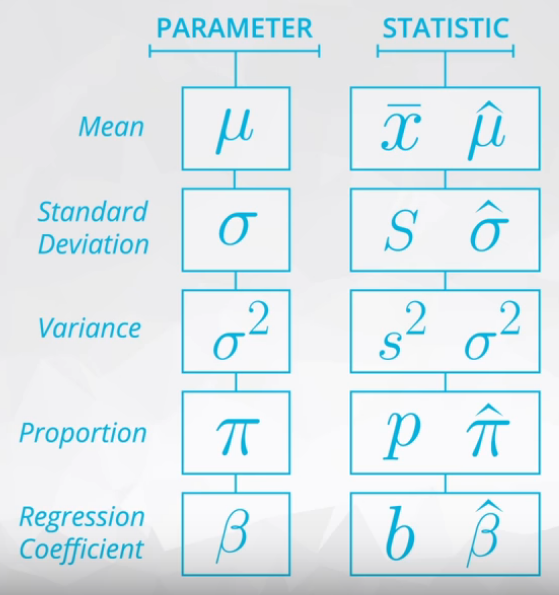
\includegraphics{01-img/c4_l10_01.png}
\caption{}
\end{figure}

Figure 1

\begin{quote}
As you saw in this video, we commonly use Greek symbols as parameters
and lowercase letters as the corresponding statistics. Sometimes in the
literature, you might also see the same Greek symbols with a ``hat'' to
represent that this is an estimate of the corresponding parameter.
\end{quote}

\subsection{Other Sampling
Distribution}\label{other-sampling-distribution}

It is possible to use other statistics.

\begin{itemize}
\tightlist
\item
  Standard Deviation
\item
  Variance
\item
  Difference in Means
\end{itemize}

The difference between parameters and statistics is the last one is
varies and the first is fixed.

\subsection{Law of Large Number}\label{law-of-large-number}

This theorem preconizes the greater the number of the samples/trials the
average of this sample will be close to the population mean. This is the
reason we have simulated samples sizes of 10,000.

\begin{itemize}
\tightlist
\item
  Increasing the size of the sample the mean of this sample will be
  closer to the population mean.
\end{itemize}

\href{https://en.wikipedia.org/wiki/Law_of_large_numbers}{Read more in
Wikipedia} and
\href{https://www.investopedia.com/terms/l/lawoflargenumbers.asp}{Investopedia}

\subsection{Central Limit Theorem}\label{central-limit-theorem}

Quite similar with the LLN theorem, but this is related to the shape of
sample. It is necessary to plot a histogram to see the miracle.

\begin{itemize}
\tightlist
\item
  Increasing the size of the sample the shape of the sample will be
  closer to a normal distribution.
\end{itemize}

\begin{figure}
\centering
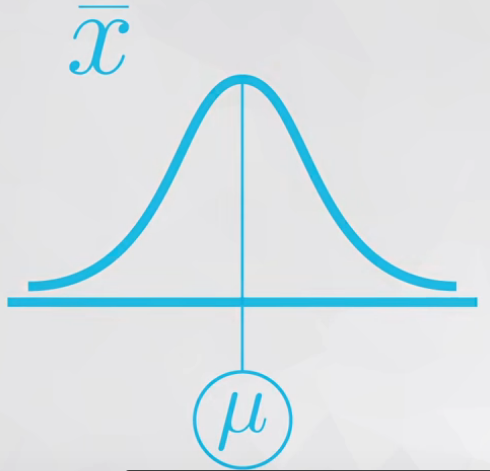
\includegraphics{01-img/c4_l10_02.png}
\caption{}
\end{figure}

Figure 2

\begin{quote}
The Central Limit Theorem states that with a large enough sample size
the sampling distribution of the mean will be normally distributed.
\end{quote}

\begin{quote}
The Central Limit Theorem actually applies for these well known
statistics:
\end{quote}

\begin{quote}
\begin{enumerate}
\def\labelenumi{\arabic{enumi}.}
\tightlist
\item
  Sample means (\(\bar x\))
\item
  Sample proportions (\(p\))
\item
  Difference in sample means (\(\bar x_1 - \bar x_2\))
\item
  Difference in sample propostions (\(p_1 - p_2\))
\end{enumerate}
\end{quote}

But is not applied to:

\begin{enumerate}
\def\labelenumi{\arabic{enumi}.}
\tightlist
\item
  Variance or Standard Deviation
\item
  Correlation coeficient
\item
  Maximum value
\end{enumerate}

\begin{quote}
And it applies for additional statistics, \textbf{but it doesn't apply
for all statistics!}. You will see more on this towards the end of this
lesson.
\end{quote}

Examples CLT in Figures 3 and 4.

\begin{figure}
\centering
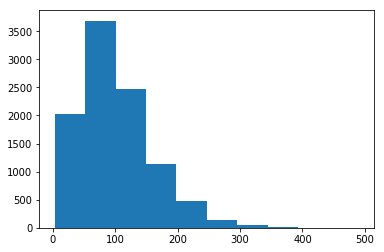
\includegraphics{01-img/c4_l10_03.png}
\caption{}
\end{figure}

Figure 3

\begin{figure}
\centering
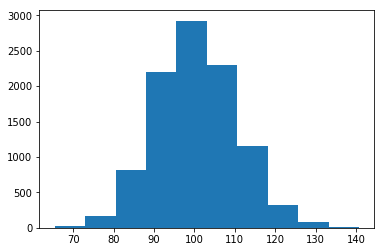
\includegraphics{01-img/c4_l10_04.png}
\caption{}
\end{figure}

Figure 4

Varying the value of the sample from 3 to 100, the bell shape could be
identified.

\subsection{Bootstrapping}\label{bootstrapping}

\begin{quote}
Bootstrapping is a technique where we sample from a group with
replacement.
\end{quote}

\begin{quote}
We can use bootstrapping to simulate the creation of sampling
distribution, which you did many times in this lesson.
\end{quote}

\begin{quote}
By bootstrapping and then calculating repeated values of our statistics,
we can gain an understanding of the sampling distribution of our
statistics.
\end{quote}

\section{\texorpdfstring{Confidence Intervals
\texttt{Lesson\ 11}}{Confidence Intervals Lesson 11}}\label{confidence-intervals-lesson-11}

Have in mind this is a part of Inference Statistical.

In this lesson we are going to use the sampling method to create our
interval of confidence. The steps is very simple:

\begin{itemize}
\tightlist
\item
  From a population gather a sample;
\item
  Based on this sample draw many new samples (e.g.~10,000);

  \begin{itemize}
  \tightlist
  \item
    The size of these 10,000 samples should be ``large'' (e.g.~200);
  \item
    You can use the \texttt{replace\ =\ True} to work with
    Bootstrapping;
  \end{itemize}
\item
  Calculate some statistics (of this 200 elements): mean or difference
  of means;
\item
  Plot a histogram of this statistics (should have 10,000 elements to
  plot).
\end{itemize}

Plotting this histogram you can take some conclusions about the data.
For example:

\begin{itemize}
\tightlist
\item
  If you decided to use difference of means, you can check if the two
  ``samples'' are equals, or greater or less than.
\end{itemize}

\begin{quote}
Assuming you control all other items of your analysis:
\end{quote}

\begin{quote}
\begin{enumerate}
\def\labelenumi{\arabic{enumi}.}
\tightlist
\item
  Increasing your sample size will decrease the width of your 2.
  confidence interval.
\item
  Increasing your confidence level (say 95\% to 99\%) will increase the
  width of your confidence interval.
\end{enumerate}
\end{quote}

\begin{quote}
You saw that you can compute:
\end{quote}

\begin{quote}
\begin{enumerate}
\def\labelenumi{\arabic{enumi}.}
\tightlist
\item
  The confidence interval \textbf{width} (Confidence Interval Width) as
  the difference between your upper and lower bounds of your confidence
  interval.
\item
  The \textbf{margin of error} (MOE) is half the confidence interval
  width, and the value that you add and subtract from your sample
  estimate to achieve your confidence interval final results. ---
  Udacity class notes
\end{enumerate}
\end{quote}

\subsection{Practical and Statistical
Significance}\label{practical-and-statistical-significance}

\begin{itemize}
\tightlist
\item
  Confidence Intervals will provide a Statistical Significance to be
  used as bedrock of a conclusion.
\item
  Practical Significance is something from outside of the Confidence
  Interval and could decide if this solution is good or not. The
  Practical Significance takes account other variables (costs, lack of
  employee, time, etc.).
\end{itemize}

\subsection{Traditional Methods vs Bootstrapping Confidence
Intervals}\label{traditional-methods-vs-bootstrapping-confidence-intervals}

The Bootstrapping Methods can perform all traditional methods of
Confidence Intervals with minors differences when the sample is a true
representation of the population.

\begin{quote}
With large sample sizes, these end up looking very similar. With smaller
sample sizes, using a traditional methods likely has assumptions that
are not true of your interval. Small sample sizes are not ideal for
bootstrapping methods though either, as they can lead to misleading
results simply due to not accurately representing your entire population
well.
\end{quote}

Traditional Methods of Confidence Intervals:

\begin{itemize}
\tightlist
\item
  T-Test: Population mean;
\item
  Two sample T-test: Comparing two means;
\item
  Z-Test;
\item
  Chi-squared test;
\item
  F-test.
\end{itemize}

\subsection{Misinterpretation of Confidence
Intervals}\label{misinterpretation-of-confidence-intervals}

The aim of a Confidence Interval is to calculate parameter, a single
value of a entire population, which could be:

\begin{itemize}
\tightlist
\item
  mean
\item
  standard deviation
\item
  difference between two means (two populations means)
\item
  Any other numeric summary in the population
\end{itemize}

Confidence Interval \textbf{do not} allow us to tell about any specific
individual of this population.

\begin{quote}
Confidence intervals take an aggregate approach towards the conclusions
made based on data, as these tests are aimed at understanding population
parameters (which are aggregate population values).
\end{quote}

\begin{quote}
Alternatively, machine learning techniques take an individual approach
towards making conclusions, as they attempt to predict an outcome for
each specific data point.
\end{quote}

\begin{quote}
In the final lessons of this class, you will learn about two of the most
fundamental machine learning approaches used in practice: linear and
logistic regression. --- Udacity Class notes
\end{quote}

\subsection{New Methods}\label{new-methods}

\subsubsection{\texorpdfstring{\texttt{.sample()}}{.sample()}}\label{sample}

Will sample a data frame, you can use \texttt{replace\ =\ True} if you
are wondering perform a bootstrap.

\begin{Shaded}
\begin{Highlighting}[]
\NormalTok{my_population.sample(}\DecValTok{100}\NormalTok{, replace }\OperatorTok{=} \VariableTok{True}\NormalTok{)}
\end{Highlighting}
\end{Shaded}

For above example the sample size is 100 and there is replacement (which
denotes it is a boootstrapping process).

\subsubsection{\texorpdfstring{\texttt{.percentile()}}{.percentile()}}\label{percentile}

This is a numpy method, and gives the percentile from a given value.

\begin{Shaded}
\begin{Highlighting}[]
\NormalTok{np.percentile(df, }\FloatTok{0.5}\NormalTok{), np.percentile(df, }\FloatTok{99.5}\NormalTok{)}
\end{Highlighting}
\end{Shaded}

There are two \texttt{.percentile()} representing a two tailed
confidence interval of 99\%.

\section{\texorpdfstring{Hypothesis Testing
\texttt{Lesson\ 12}}{Hypothesis Testing Lesson 12}}\label{hypothesis-testing-lesson-12}

Is a way to answer a given question. First step is convert/transform
this question in hypothesis. Then, gather data to answer/justify which
hypothesis are likely to be true.

\textbf{Example:} Hypothesis Examples.

My question:

\[ \text{What is the most favorite ice cream flavor?} \]

I have pose two hypothesis about ice cream.

\[H_0: \text{Chocolate is most favorite.} \\
  H_1:\text{Vanilla is most favorite.} \]

After pose hypothesis, I need to collect data to support my hypothesis
(if is \texttt{True} or \texttt{False}).

Have in mind, Confidence Intervals and Hypoteshis Testing allow us to
draw conclusions about the \textbf{population} only using \textbf{sample
data}.

\subsubsection*{\texorpdfstring{\(H_0\) - Null
hypotheses}{H\_0 - Null hypotheses}}\label{h_0---null-hypotheses}
\addcontentsline{toc}{subsubsection}{\(H_0\) - Null hypotheses}

The \(H_0\) hypothesis is also known as \emph{Null hypothesis} and this
hypothesis stand to be true \textbf{before} collect any data.

Commonly, the Null hypothesis is a statement of two groups being equal
or ``zero'' effect.

Usually, the Null hypothesis tend to hold these mathematical operators:

\begin{enumerate}
\def\labelenumi{\arabic{enumi}.}
\tightlist
\item
  \(=\)
\item
  \(\leq\)
\item
  \(\geq\)
\end{enumerate}

\subsubsection*{\texorpdfstring{\(H_1\) - Alternative
hypotheses}{H\_1 - Alternative hypotheses}}\label{h_1---alternative-hypotheses}
\addcontentsline{toc}{subsubsection}{\(H_1\) - Alternative hypotheses}

The \(H_1\) hypothesis must be competing (in comparison with the
\(H_0\)) and non-overlaping hypothesis.

This hypothesis is always associate with what we want or what we want to
prove is \texttt{True}.

Usually, the Alternative hypothesis tend to hold these mathematical
operators:

\begin{enumerate}
\def\labelenumi{\arabic{enumi}.}
\tightlist
\item
  \(\neq\)
\item
  \(>\)
\item
  \(<\)
\end{enumerate}

\textbf{Example:} Innocent until proven guilty.

My question:

\[ \text{Guilty or innocent?} \]

Which could be translated as:

\[H_0: \text{We believe everyone to be innocent initially.} \\
  H_1:\text{Guilty.} \]

Before any collect data the \(H_0\) hypothesis is \texttt{True}, and we
will collect data/evidence to test which hypothesis is supported.

\textbf{Example:} New website's version.

My question:

\[ \text{Which version of website has more traffic?} \]

In terms of hypothesis:

\[H_0: \text{The newer version has less traffic than the older version.} \\
  H_1:\text{The newer version has more traffic than the older version.} \]

Using mathematical notation and based on the average traffic (\(\mu\)).

\[H_0: \mu_{new} \leq \mu_{old} \\
  H_1: \mu_{new} > \mu_{old} \]

Bear in mind, the \(H_1\) hypothesis is our expectation (the new website
has a better performance than the older version), and now we need to
collect/gather data to analyze which hypothesis is supported.

\subsection{Type of Errors}\label{type-of-errors}

Before any explanation about erros, let's ilustrate the four (4)
potential outcome of a given \(H_0\) and \(H_1\) in Figure 1, based on
the judicial example.

\begin{figure}
\centering
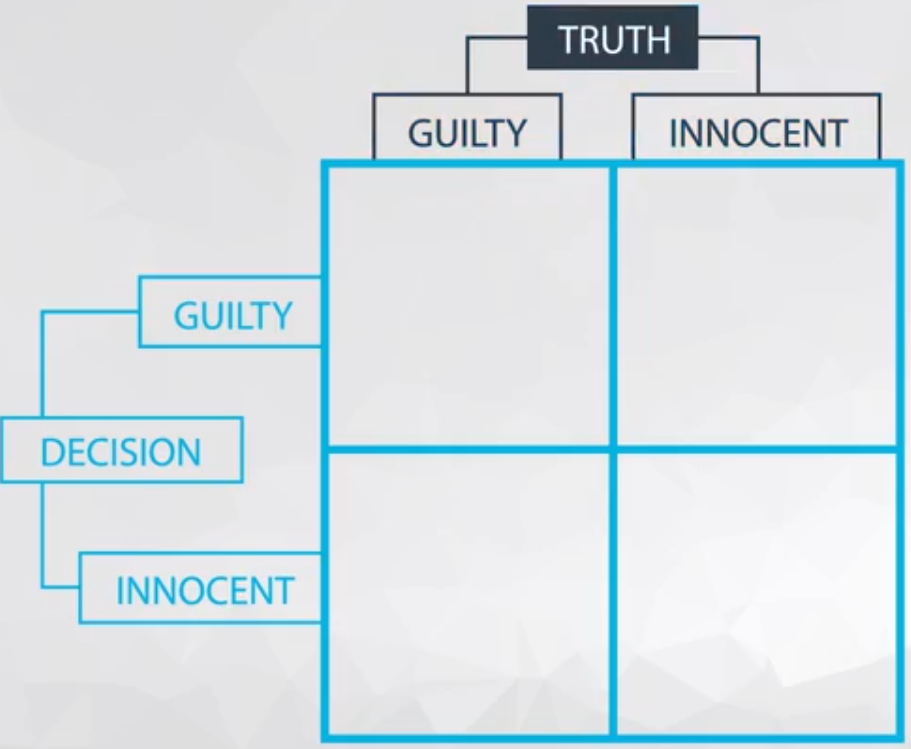
\includegraphics{01-img/c4_l12_01.png}
\caption{}
\end{figure}

Figure 1 - Four potential outcome from a Hypothesis Testing.

We can classify each of this outcome as ilustraded in Table 1.

Table 1 - Decision Classification.

GuiltyTruth

InnocentTruth

GuiltyJury

correct decision 1

mistake 1 - False Positive

InnocentJury

mistake 2 - False Negative

correct decision 2

\begin{itemize}
\tightlist
\item
  correct decision 1: Innocent person judged as innocent :+1: ;
\item
  correct decision 2: Guilty person judged as guilty :+1: ;
\item
  mistake 1: Innocent person judged as guilty :-1: ;

  \begin{itemize}
  \tightlist
  \item
    So-called \textbf{Type 1 Errors};
  \end{itemize}
\item
  mistake 2: Guilty person judged as innocent :-1: ;

  \begin{itemize}
  \tightlist
  \item
    So-called \textbf{Type 2 Errors}.
  \end{itemize}
\end{itemize}

\subsubsection{\texorpdfstring{Type 1 Errors
(\(\alpha\))}{Type 1 Errors (\textbackslash{}alpha)}}\label{type-1-errors-alpha}

This is the mistake 1 from \textbf{Table 1}.

\[ \text{The worse of the two types of errors.} \]

Put a innocent person in jail.

This happens when the \(H_1\) (alternative hypothesis) in chosen, but
actually the \(H_0\) is \texttt{True}.

\[ \text{False Positive} \]

\subsubsection{\texorpdfstring{Type 2 Errors
(\(\beta\))}{Type 2 Errors (\textbackslash{}beta)}}\label{type-2-errors-beta}

This is the mistake 2 from \textbf{Table 2}.

Let a guilty person free.

This happens when the \(H_0\) (null alternative) in chosen, but actually
the \(H_1\) is \texttt{True}.

\[ \text{False Negative} \]

\subsubsection{\texorpdfstring{Meaning of
\(\alpha\)}{Meaning of \textbackslash{}alpha}}\label{meaning-of-alpha}

\begin{quote}
What is the meaning of \(\alpha\)?
\end{quote}

This is a threshold of how many of this kind of error (the worst one!)
we are allowed to commit, leting the rest of the erros in type 2 errors.
Generally, this \(\alpha\) is quite low value, and varies according to
the field.

\begin{itemize}
\tightlist
\item
  \(\alpha\)

  \begin{itemize}
  \tightlist
  \item
    Medical: 0.01
  \item
    Business and Research: 0.05
  \end{itemize}
\end{itemize}

\textbf{Example:} Sky diving using Parachute.

In this job you are in charge of check the parachutes.You need to decide
if the parachute is well prepare to a sky dive. There are 4 possible
outcomes from your work.

\begin{itemize}
\tightlist
\item
  Accept a well prepare parachute;

  \begin{itemize}
  \tightlist
  \item
    This is a correct decision;
  \end{itemize}
\item
  Accept a shortcoming parachute;

  \begin{itemize}
  \tightlist
  \item
    This is an error type 1 the worse outcome because it will kill the
    skydiver;
  \end{itemize}
\item
  Reject a well prepare parachute;

  \begin{itemize}
  \tightlist
  \item
    This is an error type 2 because the parachute is OK but you wrongly
    reject it;
  \end{itemize}
\item
  Reject a shortcoming parachute;

  \begin{itemize}
  \tightlist
  \item
    This is a correct decision because the parachute is not well
    prepare.
  \end{itemize}
\end{itemize}

Figure 2 ilustrate it.

\begin{figure}
\centering
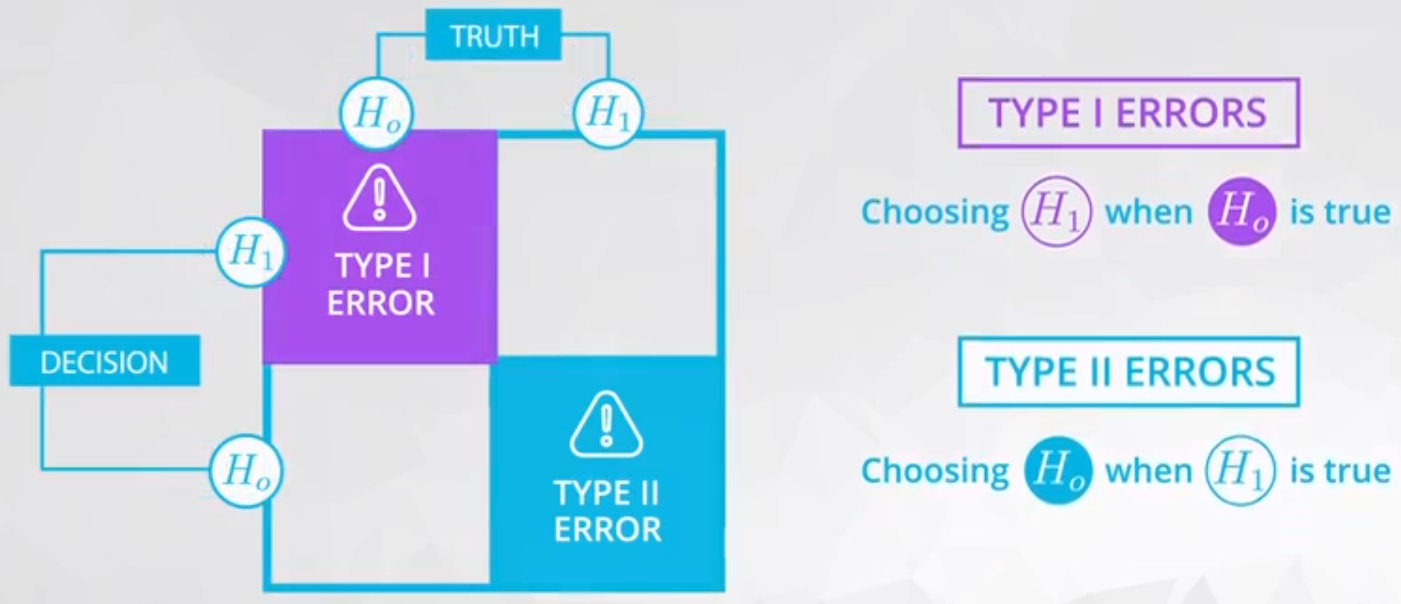
\includegraphics{01-img/c4_l12_02.png}
\caption{}
\end{figure}

Figure 2 - Four potential outcome from a Hypothesis Testing of a
Skydiver.

Bear in mind, for this example an \(\alpha\) of 0.01 is still very high.

\subsubsection{Common Hypothesis
Testing}\label{common-hypothesis-testing}

\begin{itemize}
\tightlist
\item
  T-test: population mean
\item
  Two sample t-test: difference in means
\item
  Paired t-test: Comparing after and before of a same individual
\item
  One sample z-test: population proportion
\item
  Two sample z-test: difference between population proportion
\end{itemize}

\subsection{Selecting a hypothesis}\label{selecting-a-hypothesis}

\[ \text{Which hypothesis is more likely to be True?} \]

There are two ways to select these hypothesis.

\begin{enumerate}
\def\labelenumi{\arabic{enumi}.}
\tightlist
\item
  Using Confidence Intervals: Sampling distribution of our statistics.
\item
  Simulating what we believe to be true under the null hypothesis, and
  than seeing if our data is actually consistent with that
\end{enumerate}

\subsubsection{Using Confidence
Intervals}\label{using-confidence-intervals}

Create the Confidence Intervals and check where is it.

In the example of coffee drinkers, the interval was entirely below 70,
which would suggest the null (the population mean is less than 70) is
actually true.

\begin{enumerate}
\def\labelenumi{\arabic{enumi}.}
\tightlist
\item
  Bootstrapping a sample
\item
  Calculate the statistics
\item
  Plot the histogram to visualize
\item
  Calculte the upper and lower bounds from the Confidence Intervals
\item
  Check if the \(H_0\) or \(H_1\) is in this Confidence Interval.
\end{enumerate}

\subsubsection{Traditional way}\label{traditional-way}

\begin{enumerate}
\def\labelenumi{\arabic{enumi}.}
\tightlist
\item
  We assume the \(H_0\) is \texttt{True}.
\item
  We know the sampling distribution is normal
\item
  We will use the closest value of the \(H_0\), which is almost 70.
\item
  Based on the standard deviation of the sampling distribution we could
  estimate the distribution from the \(H_0\).
\item
  Plot the histogram
\item
  Check the statistics and the hypothesis \(H_0\).
\item
  Decide to reject \(H_0\) or not.
\end{enumerate}

\subsection{P-value}\label{p-value}

Based on the Bootstrapping process the P-value could be interpreted as:
a statistics of how many samples will be higher/lower than the threshold
defined in the hypothesis.

In the exercises the P-value is an ``average'' of all 10,000 samples if
it is higher, lower, or in the tails of a specific parameter. This
``average'' (in fact is a ``vector'' of zero or one due to the
comparison) is the probability of a sample has higher/lower values from
the parameter.

Bear in mind, if 100 samples say to reject the \(H_0\) but the others
9,900 say the opposite there are a probability of 100/10,000 to incurr
in error Type 1. In other words, the 100/10,000 is the so-called
\textbf{p-value}.

The relationship between \textbf{p-value} and \(\alpha\):

\begin{itemize}
\tightlist
\item
  \textbf{p-value} \textless{} \(\alpha\) (or small p-value): Reject
  \(H_0\)
\item
  \textbf{p-value} \(\geq \alpha\) (or Large p-value): Fail to reject
  \(H_0\)
\end{itemize}

\href{https://rebeccaebarnes.github.io/2018/05/01/what-is-a-p-value}{Reference}

For a small \(\alpha\) (less than 10/10,000, for instance) probably you
will accept the \(H_0\), in the case of:

\[H_0: \mu \leq 0 \\ H_1: \mu > 0\]

There are three forms to allocate the \(\alpha\), as you can see in
Figure 3.

\begin{figure}
\centering
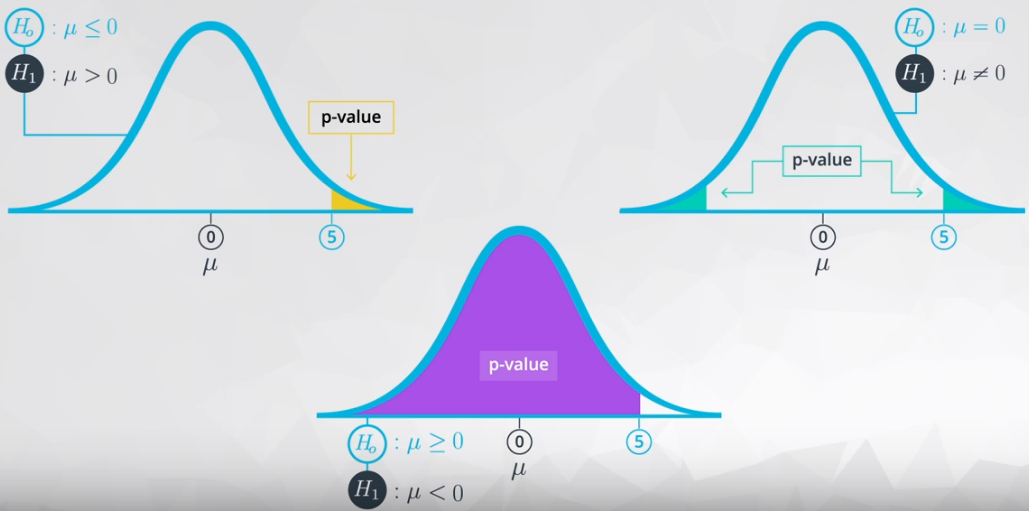
\includegraphics{01-img/c4_l12_03.png}
\caption{}
\end{figure}

\section{\texorpdfstring{A/B Testing
\texttt{Lesson\ 13}}{A/B Testing Lesson 13}}\label{ab-testing-lesson-13}

This is an application of Confidence Intervals and Hypotheses Testing.

The A/B Testing is a comparison between two groups (A and B), as
ilustrated in Figure 1.

\begin{figure}
\centering
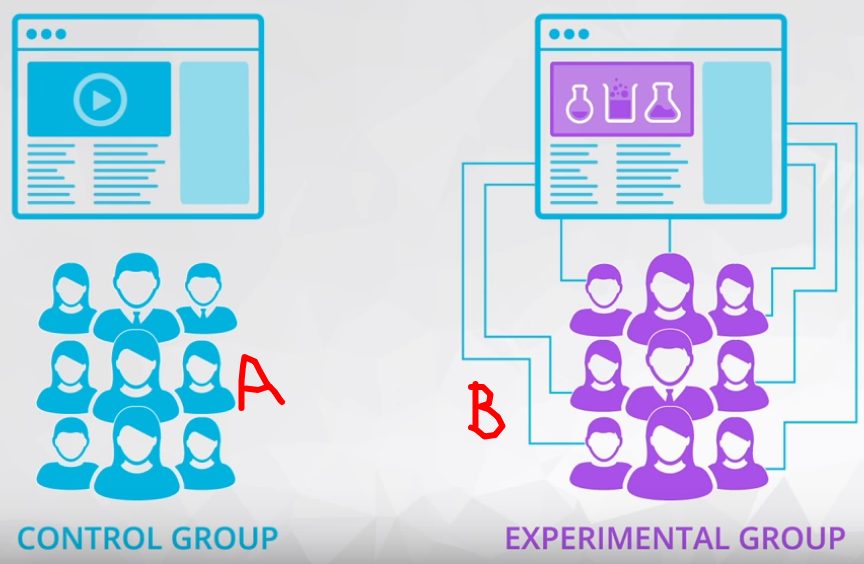
\includegraphics{01-img/c4_l13_01.png}
\caption{}
\end{figure}

Figure 1 - Two group to be tested.

\begin{quote}
A/B tests are used to test changes on a web page by running an
experiment where a control group sees the old version, while the
experiment group sees the new version. A metric is then chosen to
measure the level of engagement from users in each group. These results
are then used to judge whether one version is more effective than the
other. A/B testing is very much like hypothesis testing with the
following hypotheses:
\end{quote}

\[H_0 : \text{The new version is equal or worse than the older version.} \\
 H_1 : \text{The new version is better than the older version.} \]

Decision:

\begin{itemize}
\tightlist
\item
  If we fail to reject the null hypothesis, the results would suggest
  keeping the old version, or;
\item
  If we reject the null hypothesis, the results would suggest launching
  the change.
\end{itemize}

\subsubsection*{Drawbacks}\label{drawbacks}
\addcontentsline{toc}{subsubsection}{Drawbacks}

\begin{quote}
It can help you compare two options, but it can't tell you about an
option you haven't considered. It can also produce bias results when
tested on existing users, due to factors like change aversion and
novelty effect.
\end{quote}

\begin{quote}
\begin{itemize}
\tightlist
\item
  Change Aversion: Existing users may give an unfair advantage to the
  old version, simply because they are unhappy with change, even if it's
  ultimately for the better.
\item
  Novelty Effect: Existing users may give an unfair advantage to the new
  version, because they're excited or drawn to the change, even if it
  isn't any better in the long run.
\end{itemize}
\end{quote}

\subsection{Example: New Homepage}\label{example-new-homepage}

The Audacity company want to perform an A/B Testing of two versions of a
new homepage.

\[H_0 : CRT_{new} - CTR_{old} \leq 0 \\
  H_1 : CRT_{new} - CTR_{old} > 0\]

Where CRT stands to Click Through Rate.

There are two version: \texttt{control} and \texttt{experiment}.

The difference between the CRT is about 0.03.

\subsubsection*{Bootstrapping}\label{bootstrapping-1}
\addcontentsline{toc}{subsubsection}{Bootstrapping}

\textbf{Example:} New version of Home page.

The bootstrapping provide a histogram presented in Figure 2.

\begin{figure}
\centering
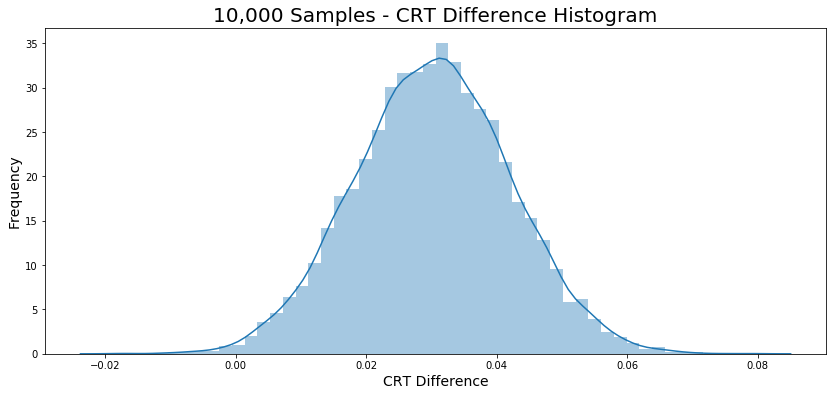
\includegraphics{01-img/c4_l13_02.png}
\caption{}
\end{figure}

The null hypothesis histogram is showed in Figure 3.

\begin{figure}
\centering
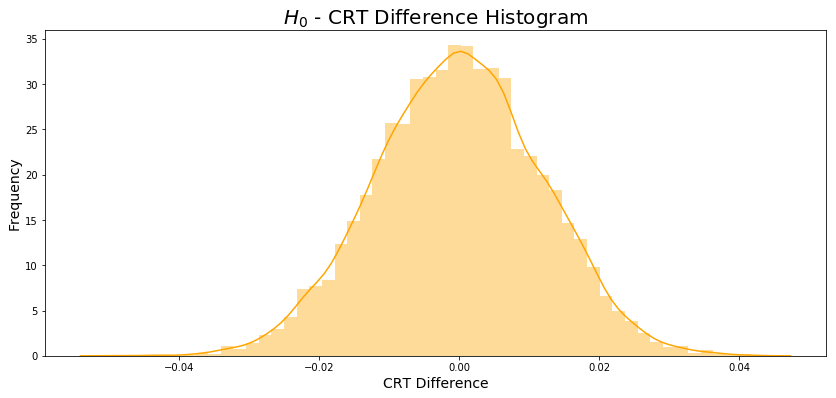
\includegraphics{01-img/c4_l13_03.png}
\caption{}
\end{figure}

Finally, Figure 4 ilustrate both histogram.

\begin{figure}
\centering
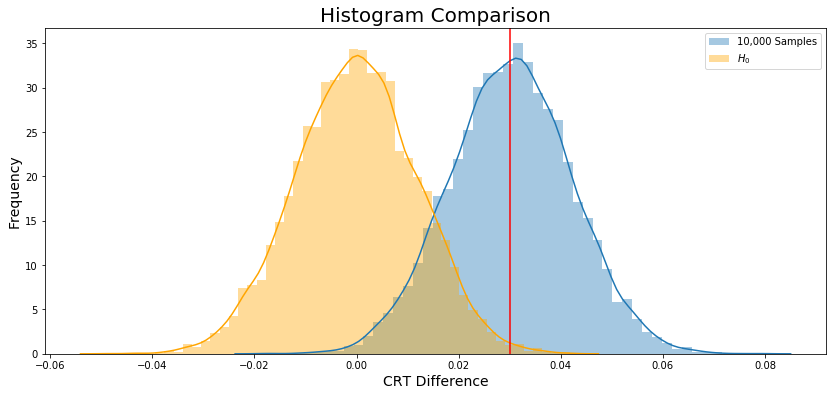
\includegraphics{01-img/c4_l13_04.png}
\caption{}
\end{figure}

\subsubsection*{P-value}\label{p-value-1}
\addcontentsline{toc}{subsubsection}{P-value}

Founded on the entire population (excepting the duplicated user id,
etc.), I have calculated the \texttt{diff}.

\begin{verbatim}
diff = experiment_crt - control_crt = 0.030034443684015644
\end{verbatim}

The \texttt{diff} could be interpreted as a threshold which I will use
as delimiter, to do it I will calculate the proportion of \(H_0\)
(orange graph) that has a difference between CRT's higher than
\texttt{diff}.

For this reason, I will calculate the average of a list of
\texttt{bool}, which will return the proportion I want.

Based on the \texttt{p\_value} of 0.5\% we reject the \(H_0\).

\begin{quote}
\textbf{Conclusion:} Audacity should launch the new version of the home
page.
\end{quote}

\subsection{Example: Average Reading
Time}\label{example-average-reading-time}

Same idea, two version of a website, one \texttt{control} and other
\texttt{experiment}.

\begin{itemize}
\tightlist
\item
  Average Reading time of control: 115.38637100678429
\item
  Average Reading time of experiment: 131.3208410471793
\item
  Difference observed: 15.9
\end{itemize}

On average, visitor using the experiment version of website spent almost
16 more seconds.

Hypotheses posed:

\[H_0 : ART_{new} - ART_{old} \leq 0 \\
  H_1 : ART_{new} - ART_{old} > 0\]

Where ART stands to Average Reading Time.

\subsubsection*{Bootstrapping}\label{bootstrapping-2}
\addcontentsline{toc}{subsubsection}{Bootstrapping}

Let's apply the bootstrapping, and plot a histogram in Figure 5.

\begin{figure}
\centering
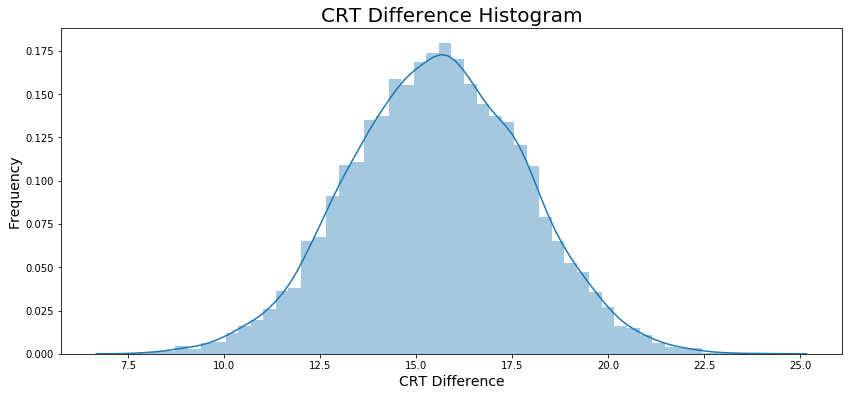
\includegraphics{01-img/c4_l13_05.png}
\caption{}
\end{figure}

The null hypothesis histogram is showed in Figure 6.

\begin{figure}
\centering
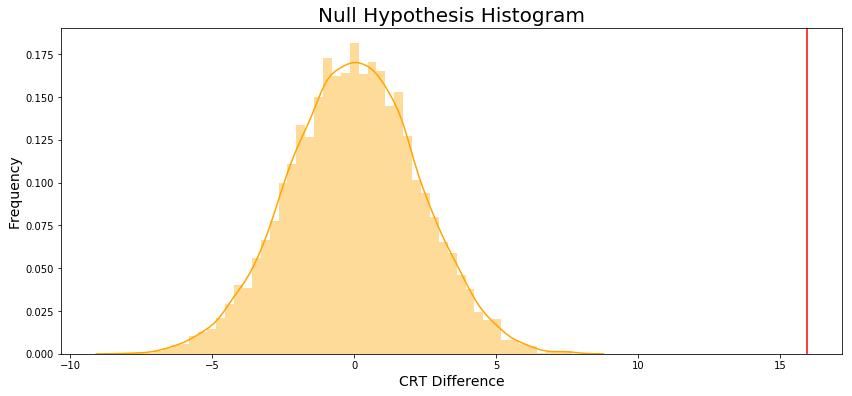
\includegraphics{01-img/c4_l13_06.png}
\caption{}
\end{figure}

Finally, Figure 7 ilustrate both histogram.

\begin{figure}
\centering
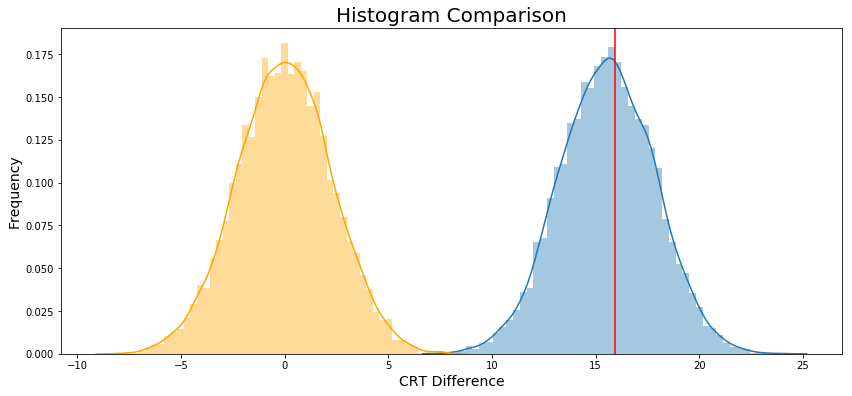
\includegraphics{01-img/c4_l13_07.png}
\caption{}
\end{figure}

\subsubsection*{P-value}\label{p-value-2}
\addcontentsline{toc}{subsubsection}{P-value}

The \texttt{p\_value} is zero.

\begin{quote}
\textbf{Conclusion:} Reject the \(H_0\) because p\_value \textless{}
\(\alpha\)
\end{quote}

Where \(\alpha\) is 0.05.

\subsection{Example: Enrollment Rate}\label{example-enrollment-rate}

This is an example to show a case where the \(H_0\) is failed to reject.

I will use the same principle of CRT to evalute the Enrollment rate.

\begin{itemize}
\tightlist
\item
  Enrollment rate control: 0.23452157598499063
\item
  Enrollment rate experiment: 0.2642986152919928
\item
  Difference observed: 0.02977703930700215
\end{itemize}

Hypotheses posed:

\[H_0 : ER_{new} - ER_{old} \leq 0 \\
  H_1 : ER_{new} - ER_{old} > 0\]

Where ER stands to Enrollment Rate.

\subsubsection*{Bootstrapping}\label{bootstrapping-3}
\addcontentsline{toc}{subsubsection}{Bootstrapping}

Let's apply the bootstrapping, and plot a histogram in Figure 8.

\begin{figure}
\centering
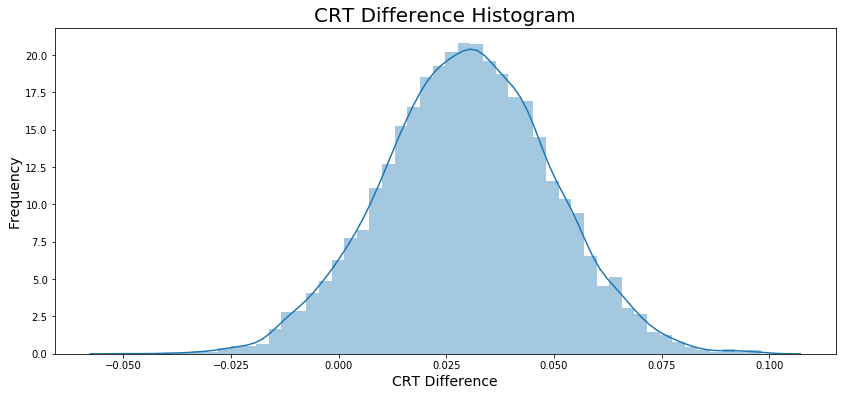
\includegraphics{01-img/c4_l13_08.png}
\caption{}
\end{figure}

The null hypothesis histogram is showed in Figure 9.

\begin{figure}
\centering
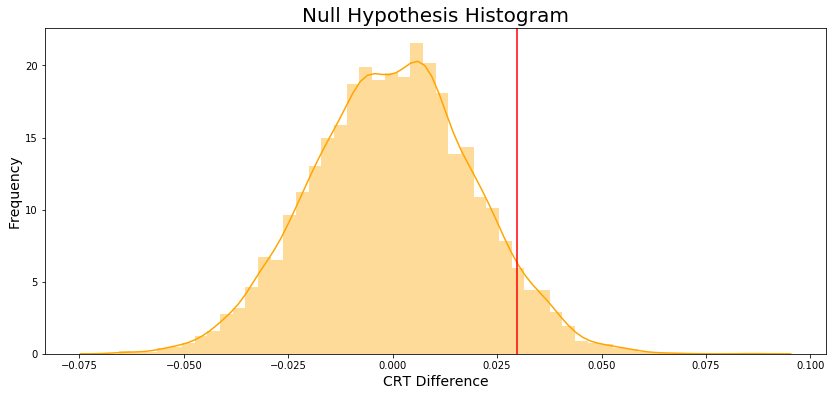
\includegraphics{01-img/c4_l13_09.png}
\caption{}
\end{figure}

Finally, Figure 10 ilustrate both histogram.

\begin{figure}
\centering
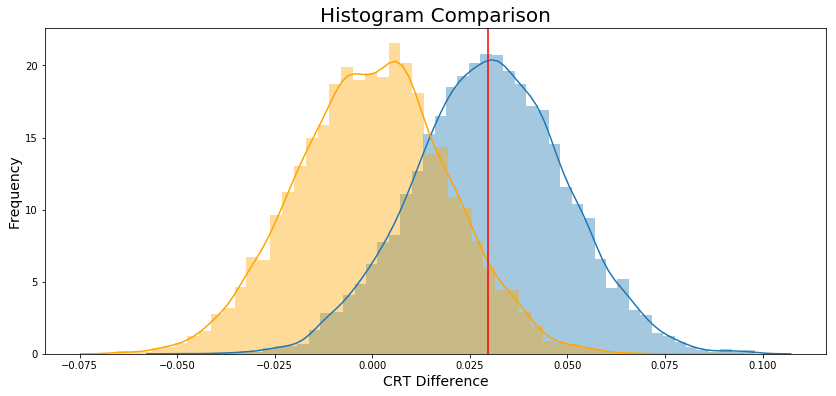
\includegraphics{01-img/c4_l13_10.png}
\caption{}
\end{figure}

\subsubsection*{P-value}\label{p-value-3}
\addcontentsline{toc}{subsubsection}{P-value}

The \texttt{p\_value} is 0.0624.

\begin{quote}
\textbf{Conclusion:} Due to p\_value \textgreater{} \(\alpha\) we fail
to reject \(H_0\).
\end{quote}

Where \(\alpha\) is 0.05.

\subsection{Bonferroni Correction}\label{bonferroni-correction}

\begin{quote}
If you remember from the previous lesson, the Bonferroni Correction is
one way we could handle experiments with multiple tests, or metrics in
this case. To compute the new bonferroni correct alpha value, we need to
divide the original alpha value by the number of tests.
\end{quote}

The new \(\alpha\) will be:

\[\alpha_{adjusted} = \frac{\alpha}{4} = \frac{0.05}{4} = 0.0125\]

Based on the several test we have done:

\begin{itemize}
\tightlist
\item
  Enrollment Rate: 0.0624 (Read the Jupyther Notebook)
\item
  Average Reading Duration: 0 (Read the Jupyther Notebook)
\item
  Average Classroom Time: 0.0384 (Read the Jupyther Notebook)
\item
  Completion Rate: 0.0846 (Read the Jupyther Notebook)
\end{itemize}

This new \(\alpha\) will generate only \textbf{one} A/B Testing
statistical significant.

\begin{longtable}[]{@{}ccccc@{}}
\toprule
New Feature & p value & \(\alpha_{adjusted}\) & Result &
\(H_0\)\tabularnewline
\midrule
\endhead
Enrollment Rate & 0.0624 & 0.0125 & \textgreater{} & Fail to reject
\(H_0\)\tabularnewline
Average Reading Duration & 0 & 0.0125 & \textless{} & Reject
\(H_0\)\tabularnewline
Average Classroom Time & 0.0384 & 0.0125 & \textgreater{} & Fail to
reject \(H_0\)\tabularnewline
Completion Ratee & 0.0846 & 0.0125 & \textgreater{} & Fail to reject
\(H_0\)\tabularnewline
\bottomrule
\end{longtable}

This is the reason the Bonferroni method is considered conservative.

\subsection{Difficulties in A/B
Testing}\label{difficulties-in-ab-testing}

\begin{quote}
As you saw in the scenarios above, there are many factors to consider
when designing an A/B test and drawing conclusions based on its results.
To conclude, here are some common ones to consider.
\end{quote}

\begin{quote}
\begin{itemize}
\tightlist
\item
  Novelty effect and change aversion when existing users first
  experience a change
\item
  Sufficient traffic and conversions to have significant and repeatable
  results
\item
  Best metric choice for making the ultimate decision (eg. measuring
  revenue vs.~clicks)
\item
  Long enough run time for the experiment to account for changes in
  behavior based on time of day/week or seasonal events.
\item
  Practical significance of a conversion rate (the cost of launching a
  new feature vs.~the gain from the increase in conversion)
\item
  Consistency among test subjects in the control and experiment group
  (imbalance in the population represented in each group can lead to
  situations like Simpson's Paradox) --- Udacity notebook
\end{itemize}
\end{quote}

\section{\texorpdfstring{Regression
\texttt{Lesson\ 14}}{Regression Lesson 14}}\label{regression-lesson-14}

Bear in mind, regression is a subject of the Supervised branch of
Machine Learning. Figure 1 shows a simple big picture.

\begin{figure}
\centering
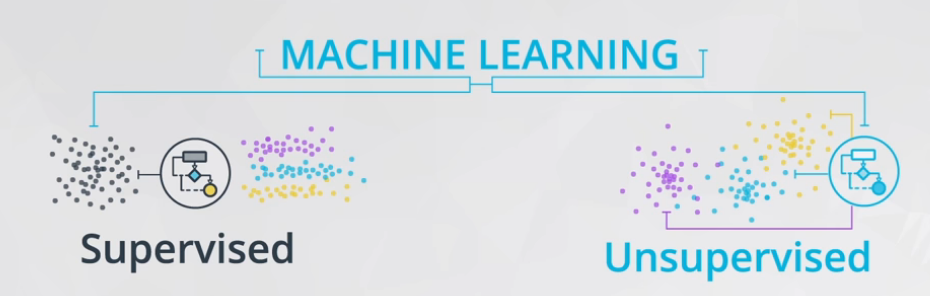
\includegraphics{01-img/c4_l14_01.png}
\caption{}
\end{figure}

Figure 1 - Machine Learning Branches.

Some hot points in these two branches (there are other branches, but
these two are the most know).

\begin{itemize}
\tightlist
\item
  Supervised: A machine learning technique where we are attempting to
  predict a label based on inputs.

  \begin{itemize}
  \tightlist
  \item
    Predict fraudulent transactions
  \item
    Predict chance of default on a loan
  \item
    Predict home prices
  \end{itemize}
\item
  Unsupervised: A machine learning technique where we are attempting to
  group together unlabeled data based on similar characteristics.

  \begin{itemize}
  \tightlist
  \item
    Customer segmentation
  \item
    Group document that cover similar topics
  \end{itemize}
\end{itemize}

The Linear and Logistic Regression fall into the Supervised Machine
Learning branch.

\subsection{Introduction to Linear
Regression}\label{introduction-to-linear-regression}

\begin{itemize}
\tightlist
\item
  Response variable or dependent (y): The variable you are interested in
  predicting, and;
\item
  Explanatory variable or independent (x): The variable used to
  predicted the response.
\end{itemize}

\begin{quote}
A common way to visualize the relationship between two variables in
linear regression is using a scatterplot. You will see more on this in
the concepts ahead. --- Udacity notebook
\end{quote}

Figure 2 shows an example of a scatter plot.

\begin{figure}
\centering
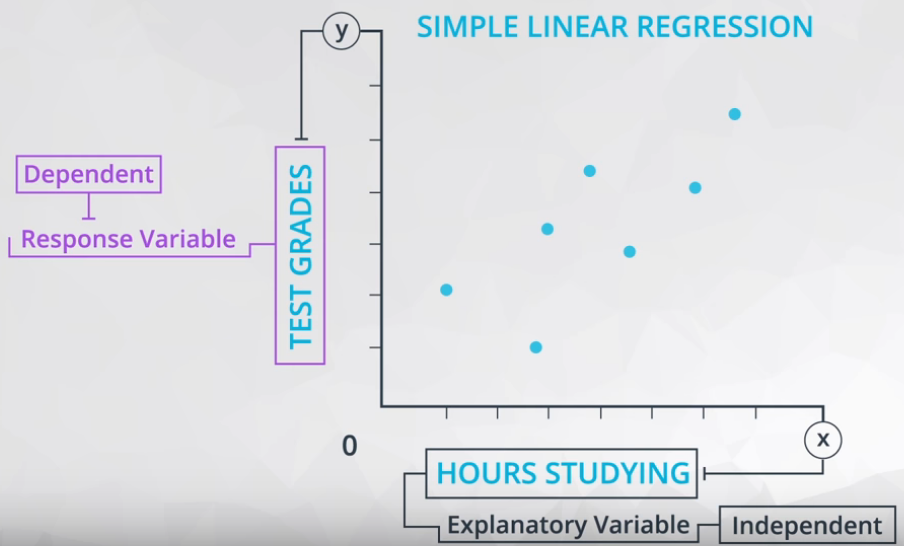
\includegraphics{01-img/c4_l14_02.png}
\caption{}
\end{figure}

Figure 2 - Hours studying vs Test grades.

\subsubsection{Scatter Plot}\label{scatter-plot}

\begin{quote}
Scatter plots are a common visual for comparing two quantitative
variables. A common summary statistic that relates to a scatter plot is
the \textbf{correlation coefficient} commonly denoted by \texttt{r}.

Though there are a few different ways to measure correlation between two
variables, the most common way is with Pearson's correlation
coefficient. Pearson's correlation coefficient provides the:

\begin{enumerate}
\def\labelenumi{\arabic{enumi}.}
\tightlist
\item
  Strength
\item
  Direction
\end{enumerate}

of a linear relationship. Spearman's Correlation Coefficient does not
measure linear relationships specifically, and it might be more
appropriate for certain cases of associating two variables. --- Udacity
notebook
\end{quote}

Figure 3 shows an example of strong positive relationship.

\begin{figure}
\centering
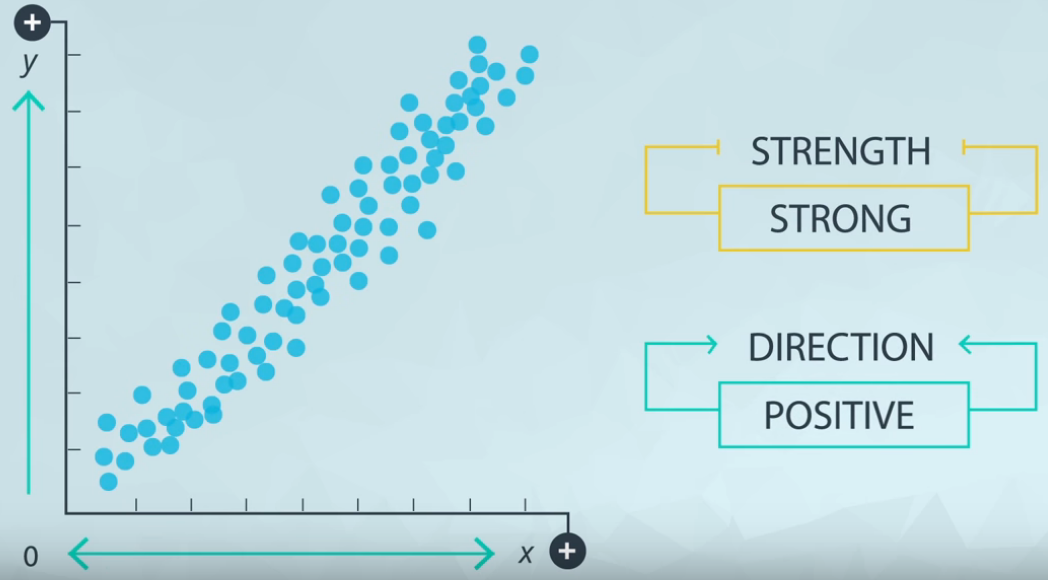
\includegraphics{01-img/c4_l14_03.png}
\caption{}
\end{figure}

Figure 3 - Strong and Positive Relantionship.

When x increase y also increase, and the points is very close from each
other. Figure 4 shows the opposite of positive direction.

\begin{figure}
\centering
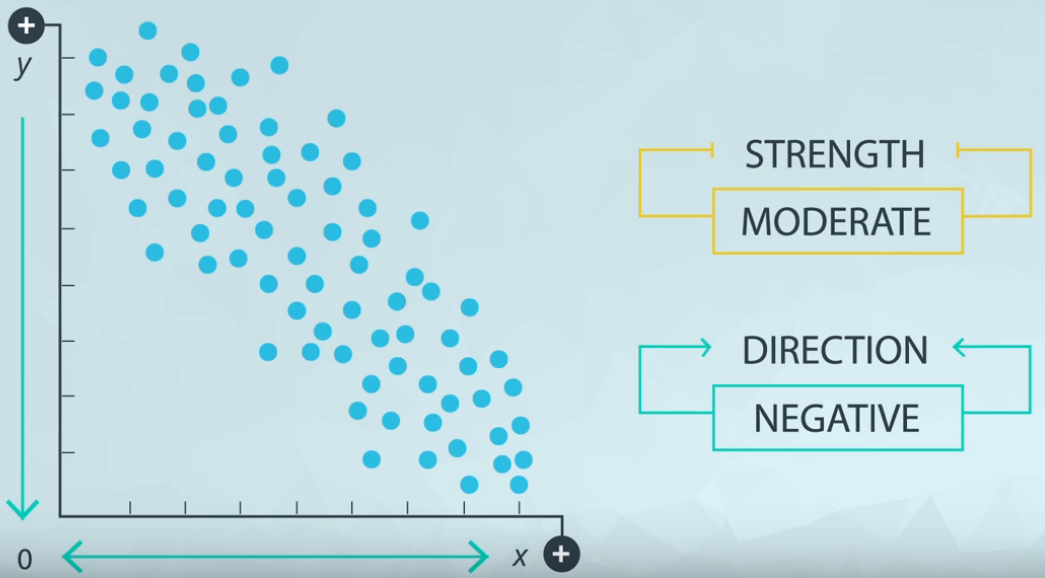
\includegraphics{01-img/c4_l14_04.png}
\caption{}
\end{figure}

Figure 4 - Moderate and Negative Relantionship.

When x increase y decrease, and the points is a bit sparse. Figure 5
shows an example of scatter plot with weak strength.

\begin{figure}
\centering
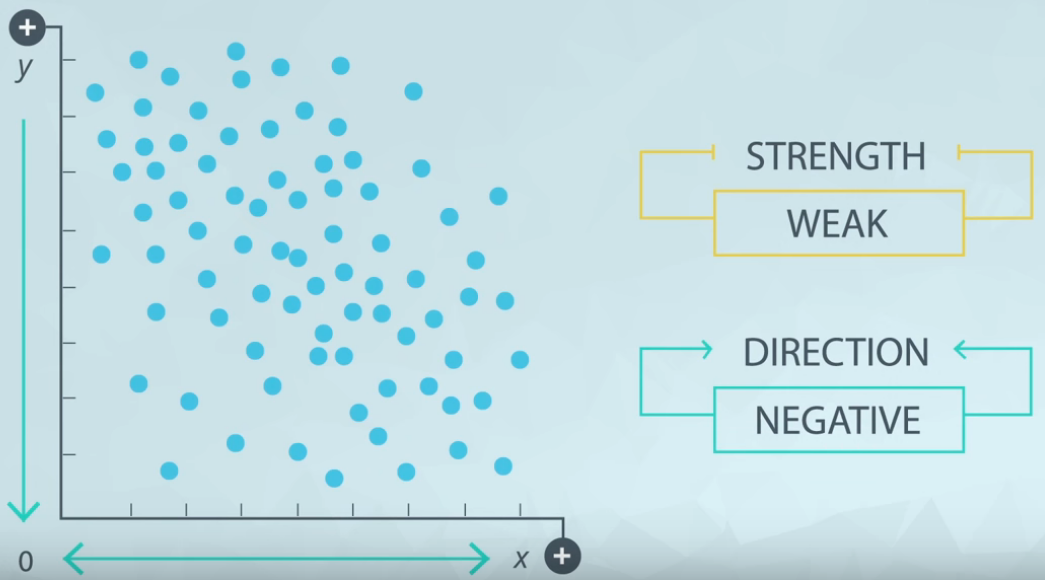
\includegraphics{01-img/c4_l14_05.png}
\caption{}
\end{figure}

Figure 5 - Weak and Negative (??) Relantionship.

Both, strength and direction is capture by the correlation (\texttt{r}).

\begin{itemize}
\tightlist
\item
  Correlation

  \begin{itemize}
  \tightlist
  \item
    Varies from -1 to +1;
  \item
    Values close to -1 and +1 are very strong;
  \item
    The signal (positive or negative) means the direction.
  \end{itemize}
\end{itemize}

\begin{figure}
\centering
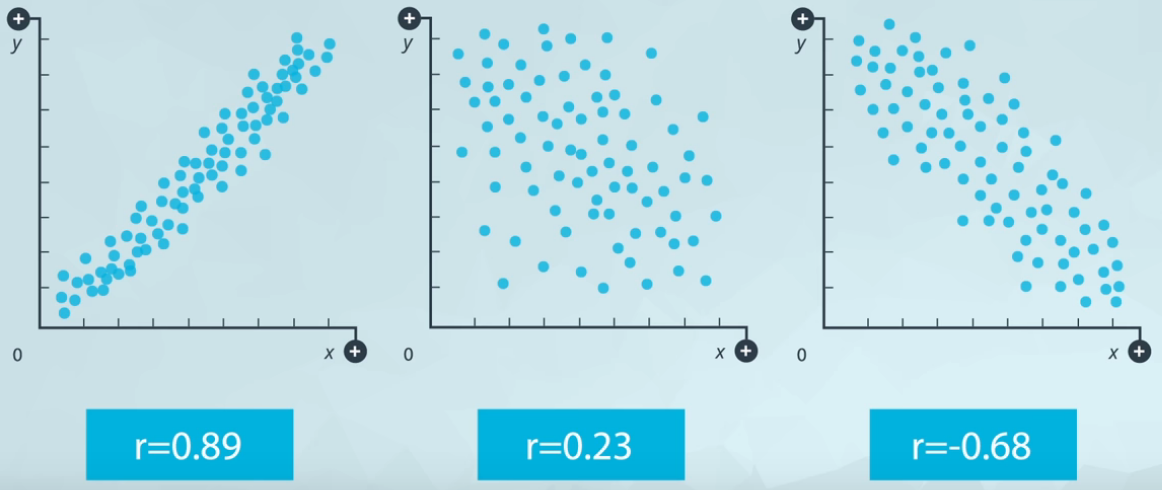
\includegraphics{01-img/c4_l14_06.png}
\caption{}
\end{figure}

Figure 6 - Example of Correlation.

\subsection{Correlation Coefficients}\label{correlation-coefficients}

This is highly field-dependent measure and these values are a general
rule of thumbs.

Have in mind, in social sciences is very difficult to find a strong
correlation (probably because human are very complex and hard to
understand).

\begin{itemize}
\tightlist
\item
  Strong: \(0.7 \leq |r| \leq 1.0\)
\item
  Moderate: \(0.3 \leq |r| \leq .7\)
\item
  Weak: \(0.0 \leq |r| \leq 0.3\)
\end{itemize}

Sometimes a plot could help a lot, Figure 7 shows an example of two
graphs with same correlation coefficients.

\begin{figure}
\centering
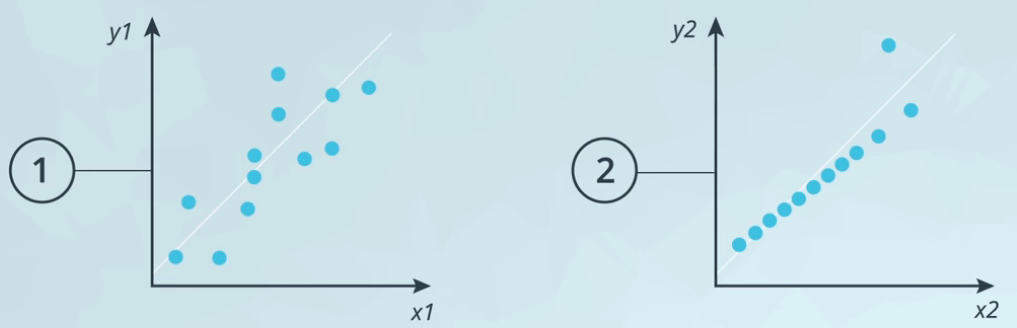
\includegraphics{01-img/c4_l14_07.png}
\caption{}
\end{figure}

Figure 7 - Two Graphics with same Correlation Coefficients.

This problem presented in Figure 6 is part of the
\href{https://en.wikipedia.org/wiki/Anscombe\%27s_quartet}{Anscombe's
Quartet} images.

\subsection{Coefficients}\label{coefficients}

A Linear Regression is a way to estimate the values of some
coefficients:

\begin{itemize}
\tightlist
\item
  Intercept: The expected value of the response when the explanatory
  variable is 0 (zero);

  \begin{itemize}
  \tightlist
  \item
    \(b_0:\) statistic value (sample)
  \item
    \(\beta_0:\) parameter value (population)
  \end{itemize}
\item
  Slope: The expected change in the response for each 1 unit increase in
  the explanatory variable.

  \begin{itemize}
  \tightlist
  \item
    \(b_1:\) statistic value (sample)
  \item
    \(\beta_1:\) parameter value (population)
  \end{itemize}
\end{itemize}

Based on the Intercept and Slope, the Linear Regression equation is
presented in equation (1).

\[ \hat y = b_0 + b_1x \]

Where: * \(\hat y:\) is the predicted value of the response from the
line. * \(y:\) is an actual response value for a data point in our
dataset (not a prediction from our line). * \(b_0:\) is the intercept. *
\(b_1:\) is the slope. * \(x_1:\) is the explanatory variable.

Figure 8 ilustrate this equation in a picture.

\begin{figure}
\centering
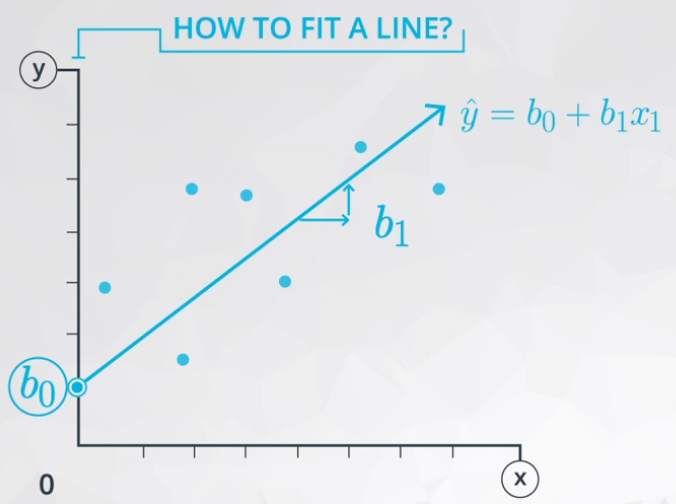
\includegraphics{01-img/c4_l14_08.png}
\caption{}
\end{figure}

Figure 8 - Linear Model and Equation.

\subsection{Least-squares}\label{least-squares}

\section{\texorpdfstring{Multilinear Regression
\texttt{Lesson\ 15}}{Multilinear Regression Lesson 15}}\label{multilinear-regression-lesson-15}

This is a generalization of the simple Linear Model, which allows us to
use several explanatory variables, as you can see an example of Multiple
Linear Regression in equation (1).

\[ \hat y = b_0 + b_1x_1 + b_2x_2 + b_3x_3 + b_4x_4 \tag{1} \]

Figure 1 ilustrate the variables which could be used to predic the
house's price.

\begin{figure}
\centering
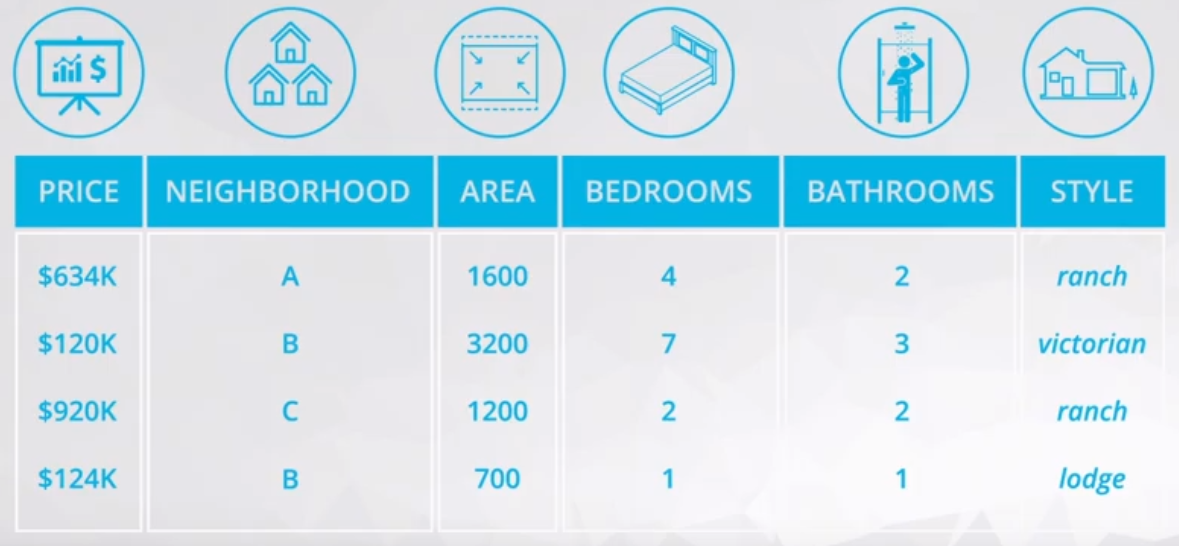
\includegraphics{01-img/c4_l15_01.png}
\caption{}
\end{figure}

Figure 1 - House Price Dataset.

Have in mind, in this table above there are quantitative and categorical
variables.

\begin{itemize}
\tightlist
\item
  Quantitative:

  \begin{itemize}
  \tightlist
  \item
    Price, Area, Bedrooms, and Bathrooms;
  \end{itemize}
\item
  Categorical:

  \begin{itemize}
  \tightlist
  \item
    Neighborhood and Style.
  \end{itemize}
\end{itemize}

All these variables will be used to predict the house's price, to do it
so it is necessary a little of linear algebra, as you can see in the
Figure 2.

\begin{figure}
\centering
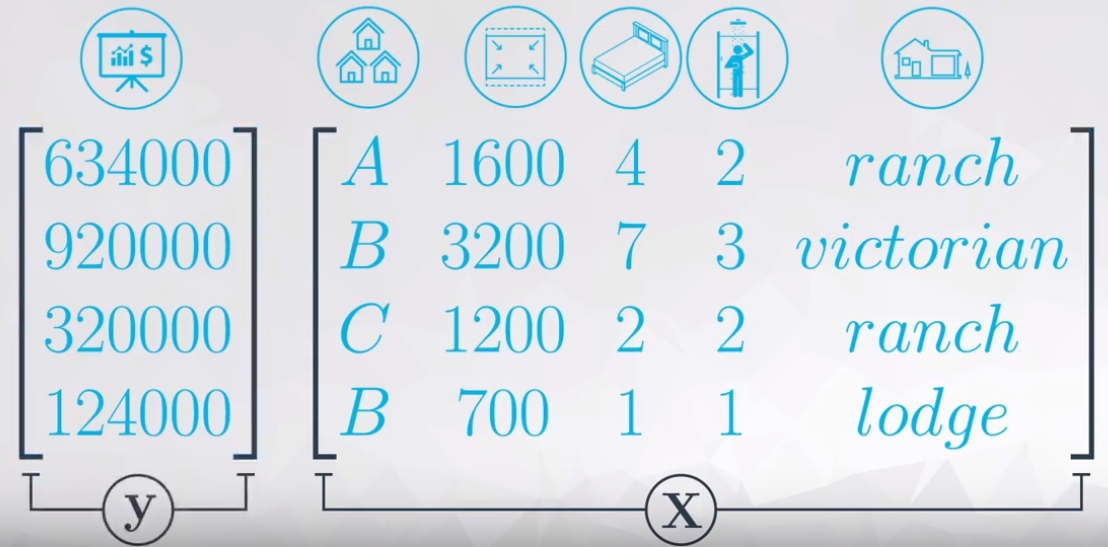
\includegraphics{01-img/c4_l15_02.png}
\caption{}
\end{figure}

Figure 2 - Matrix notation.

Where:

\begin{itemize}
\tightlist
\item
  \(\bold X:\) Matrix of inputs;
\item
  \(\bold y:\) Vector of response that we want to predict.
\end{itemize}

After many steps of linear algebra, equation (2) resume the \(\beta\)
calculation.

\[ \beta = (\bold X' \bold X)^{-1} \bold X \bold y \tag{2}\]

Have in mind, the coefficients calculated in \(\beta\) are the same
shown in Figure 3 in column \texttt{coef}.

\subsubsection*{Interpretation}\label{interpretation}
\addcontentsline{toc}{subsubsection}{Interpretation}

Figure 3 presents outputs from the OLS of a generic dataset
(house\_prices.csv).

\begin{figure}
\centering
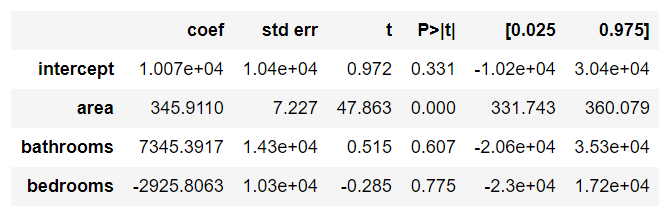
\includegraphics{01-img/c4_l15_03.png}
\caption{}
\end{figure}

Figure 3 - Coefficients, Standard Errors, etc.

\begin{quote}
In this video, the coefficients were all positive. Therefore, we can
interpret each coefficient as the \textbf{predicted increase in the
response for every one unit increase in the explanatory variable,
holding all other variables in the model constant.}
\end{quote}

This principles is the so-called
\href{https://en.wikipedia.org/wiki/Ceteris_paribus}{\emph{ceteris
paribus}}.

\begin{quote}
\emph{Ceteris paribus or caeteris paribus is a Latin phrase meaning
``other things equal''. English translations of the phrase include ``all
other things being equal'' or ``other things held constant'' or ``all
else unchanged''. A prediction or a statement about a causal, empirical,
or logical relation between two states of affairs is ceteris paribus if
it is acknowledged that the prediction, although usually accurate in
expected conditions, can fail or the relation can be abolished by
intervening factors.} --- Wikipedia
\end{quote}

\subsubsection{Statistical Significance}\label{statistical-significance}

Analogous to the simple Linear Model, it is important to analyse the
\texttt{p-values} of each variable. Figure 4 shows the
\texttt{p-values}.

\begin{figure}
\centering
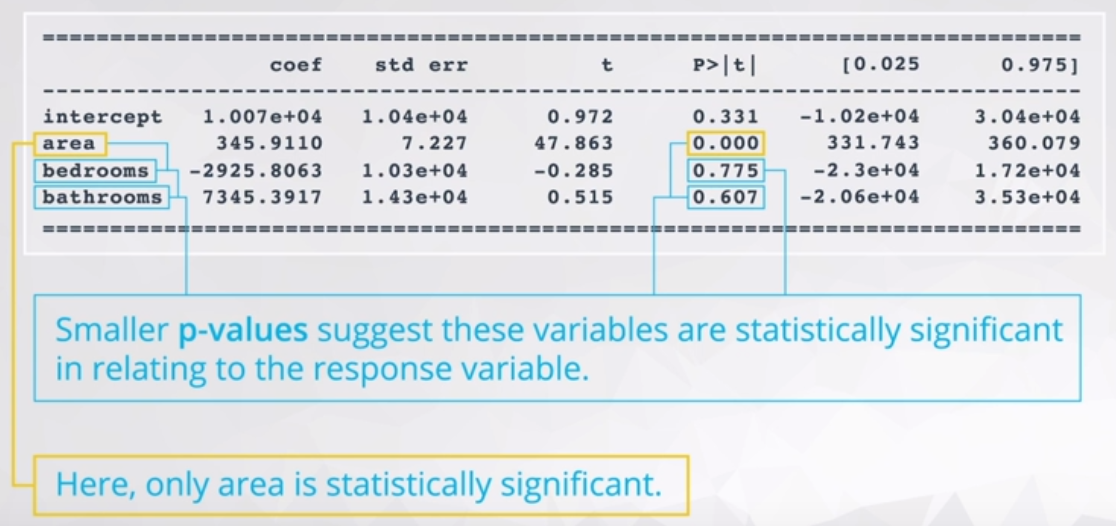
\includegraphics{01-img/c4_l15_04.png}
\caption{}
\end{figure}

Figure 4 - Statistical Significance.

As you can see, most of the variable do not have lower
\texttt{p-values}, which suggest these variables are not statistically
signigicant to the response variable. In this example, only
\texttt{area} reject \(H_0\) the others variables failed to reject
\(H_0\).

Signigicant bivariate relationships are \textbf{not} always signigicant
in Multiple Linear Regression.

\subsection{Dummy Variable}\label{dummy-variable}

This is a method to insert categorical variables in Multiple Linear
Regressions. We will use 0 and 1 to encode this Dummy Variable, which
will work creating new columns for each category of the variable. Figure
5 shows an example.

Figure 5 - Converting Categorical Variable to Dummy Variable.

Remember, the C columns is not necessary because is a complement of the
other two columns (A and B). The dropped columns (in this case the C
column) is the so-called \textbf{baseline}. What you need to understand
about the \textbf{baseline} is:

\begin{quote}
The coefficients you obtain from the output of your multiple linear
regression models are then an indication of how the encoded levels
compare to the baseline level (the dropped level). --- Udacity Notebook
\end{quote}

The mathematical reason to drop one columns is to garantee the
\(\bold X\) matrix is invertible.

\subsubsection*{Interpretation}\label{interpretation-1}
\addcontentsline{toc}{subsubsection}{Interpretation}

The baseline will be used to calculate the real coefficients of each
Dummy variable. Figure 6 shows an example of output of a Multiple Linear
Regression.

Figure 6 - Example of Coefficients from a Dummies Variables.

The intercept is the value of the baseline (in other words it is the
coefficient of A). To calculate the other coefficients you need to
subtract the baseline from each coefficient.

\begin{itemize}
\tightlist
\item
  Coefficient A: 5.411e+05
\item
  Coefficient B: 5.411e+05 - 5.295e+05 = 1070600.0
\item
  Coefficient C: 5.411e+05 - 332.36 = 540767.6406
\end{itemize}

Coef C \textless{} Coef A \textless{} Coef B

Each of the coefficients provided by the OLS is a comparison with the
baseline.

In a more complex example as presented in Figure 7.

Figure 7 - Dummies Variables from two categories.

There are ``two'' \textbf{baseline} variables: \texttt{A} and
\texttt{ranch}.

\begin{itemize}
\tightlist
\item
  Coefficient A: -383300.0
\item
  Coefficient B: -383300.0 + 5.229e5 = 139600.0
\item
  Coefficient C: -383300.0 - 7168.63 = -390500.0
\item
  ranch: -383300.0
\item
  lodge: -383300.0 + 1.685e5 = -214800.0
\item
  victorian: -383300.0 + 7.056e4 = -312770.0
\end{itemize}

\subsection{Problems in Multiple Linear
Regression}\label{problems-in-multiple-linear-regression}

Problems is sensible to the application of this Multiple Linear
Regression.

\begin{itemize}
\tightlist
\item
  What is your model for?

  \begin{itemize}
  \tightlist
  \item
    Understand how is related x and y
  \item
    Best predict the response variable
  \item
    Which variable is really useful in predicting your response
  \end{itemize}
\end{itemize}

Founded on the objectivies of the model, there are many possibilities of
problems, below there are some common problems.

\begin{itemize}
\tightlist
\item
  A linear relationship does not exist
\item
  Correlated errors
\item
  Non-constant variance
\item
  Outliers
\item
  Multicollinearity
\end{itemize}

\subsubsection*{Multicollinearity}\label{multicollinearity}
\addcontentsline{toc}{subsubsection}{Multicollinearity}

Generally, we assume the explanatory variables are all uncorrelated with
one another, but we want these explanatory variables are correlated with
the responer variable.

An example of possible multicollinearity:

\begin{quote}
We expected a bigger number of bedrooms and bathrooms when the house
area increases.
\end{quote}

There are two ways to identify the multicollinearity:

\begin{itemize}
\tightlist
\item
  Plotting the scatterplot matrix, or;
\item
  Calculating the
  \href{https://en.wikipedia.org/wiki/Variance_inflation_factor}{Variance
  Inflation Factors} (VIFs)
\end{itemize}

\textbf{Scatterplot}

Figure 8 shows the scatter plot of area, bedrooms, and bathrooms.

Figure 8 - Scatterplot of area, bedrooms, and bathrooms.

All three variables have strong and positive correlation.

OK! Let's calculate the Multiple Linear Regression using \texttt{area},
\texttt{bedrooms}, and \texttt{bathrooms} as explanatory variables to
predict the \texttt{price}. Figure 9 shows the output of the
\texttt{OLS} method.

Figure 9 - Coefficients of a Multiple Linear Regression based on area,
bedrooms, and bathrooms to predict price.

Remember, we expected positive values of coefficients, but the bedrooms
coefficient is negative. This is one of the side effect of
multicollinearity, it could flip the signal, and produce a weird result.

\textbf{Calculating the VIF}

\begin{quote}
The Variance Inflation Factor (VIF) is a measure of colinearity among
predictor variables within a multiple regression. It is calculated by
taking the the ratio of the variance of all a given model's betas divide
by the variane of a single beta if it were fit alone. ---
\href{https://etav.github.io/python/vif_factor_python.html}{Ernest
Tavares Website}
\end{quote}

In other words, this means to calculate for each explanatory variable
the R-squared adopting it as response variable, and later calculate the
VIF according to the equation (3).

\[VIF_i = \frac{1}{1-R^2_i} \tag{3}\]

Where:

\begin{itemize}
\tightlist
\item
  \(i:\) intercept, area, bedrooms, and bathrooms.
\end{itemize}

This is my original equation:

\[ price = intercept + area*b_1 + bedrooms * b_2 + bathrooms * b_3 \]

Where:

\begin{itemize}
\tightlist
\item
  Explanatory variables: intercept, area, bedrooms, and bathrooms.
\item
  Response variable: price
\end{itemize}

I need to calculate the \(R^2\) for each of these equations:

\[ intercept = area*b_1 + bedrooms * b_2 + bathrooms * b_3 \\ bedrooms = intercept + area*b_1 + bathrooms * b_3 \\
bathrooms = intercept + area*b_1 + bedrooms * b_3 \\
area = intercept + bathrooms*b_1 + bedrooms * b_3 \]

The result of the \(R^2\) is presented in Table 1.

Table 1 - R-Squared used to Calculate the VIF.

\begin{longtable}[]{@{}cc@{}}
\toprule
Response Variable & \(R^2\)\tabularnewline
\midrule
\endhead
intercept & 0.8635203885901309\tabularnewline
area & 0.8167890866692036\tabularnewline
bedrooms & 0.952048682065964\tabularnewline
bathrooms & 0.9473873926707678\tabularnewline
\bottomrule
\end{longtable}

Table 2 shows the VIFs for each value of \(R^2\).

Table 2 - VIFs.

\begin{longtable}[]{@{}cc@{}}
\toprule
Response Variable & VIF\tabularnewline
\midrule
\endhead
intercept & 7.3271017529266529\tabularnewline
area & 5.458190136274525\tabularnewline
bedrooms & 20.854484153608585\tabularnewline
bathrooms & 19.006851223744377\tabularnewline
\bottomrule
\end{longtable}

\begin{quote}
When VIFs are greater than 10, this suggests that multicollinearity is
certainly a problem in your model. Some experts even suggest VIFs of
greater than 5 can be problematic. In most cases, not just one VIF is
high, rather many VIFs are high, as these are measures of how related
variables are with one another. --- Udacity notebook.
\end{quote}

In this case I will remove the bathrooms variable, and update my
equation:

\[ price = intercept + area * b_1 + bedrooms * b_2 \tag{4}\]

Following the same process, I will calculate the new \(R^2\) and later
the VIF's.

Table 3 - R-Squared used to Calculate the VIF.

\begin{longtable}[]{@{}ccc@{}}
\toprule
Response Variable & \(R^2\) & VIF\tabularnewline
\midrule
\endhead
intercept & 0.8350894909730524 & 6.063894932472694\tabularnewline
area & 0.8129232492956318 & 5.345399662089865\tabularnewline
bedrooms & 0.8129232492956316 & 5.3453996620898625\tabularnewline
\bottomrule
\end{longtable}

There is an other way to calculate this VIF's using the
\texttt{variance\_inflation\_factor} from
\texttt{statsmodels.stats.outliers\_influence}. It is much simpler to
apply this methods, but it is quite hard to understand the hidden
subject behind the scenes.

\subsection{Higher Order Terms}\label{higher-order-terms}

Adding higher order terms is a way to add non-linearity to explain the
response variable.

\begin{itemize}
\tightlist
\item
  Higher Order Terms:

  \begin{itemize}
  \tightlist
  \item
    Interactions: \(x_1x_2\)
  \item
    Quadratics: \(x^2\)
  \item
    Cubics: \(x^3\)
  \item
    Other higher orders terms: \(x^n\)
  \end{itemize}
\end{itemize}

Adding these terms could improve the response results, but it makes
harder to understand and explain the relationship between this higher
orders terms.

For instance, \(y_1\) do not have higher orders terms and \(y_2\) has a
interaction. Both equations are quite similar, except from the term
\(cx_1x_2\).

\[y_1 = ax_1 + bx_2 + d \\
  y_2 = ax_1 + bx_2 + cx_1x_2 + d\]

The derivate from each equation will return the slope coefficient.

\[\frac{\partial y_1}{\partial x_1} = a \\
  \frac{\partial y_2}{\partial x_1} = a + c \cdot x_2\]

In \(\partial y_1/\partial x_1\) the slope is constant (\(a\)), whereas
in \(\partial y_2/\partial x_1\) the slope will varies according to the
\(c \cdot x_2\).

\subsection{New Method}\label{new-method}

In this lesson the pandas package method called \texttt{.get\_dummies}
will introduced.

\subsubsection{\texorpdfstring{\texttt{.get\_dummies()}}{.get\_dummies()}}\label{get_dummies}

This method returns a Data Frame with each category of the categorical
variable as a new column.

\begin{Shaded}
\begin{Highlighting}[]
\NormalTok{pd.get_dummies(df[}\StringTok{'categorical_variable'}\NormalTok{])}
\end{Highlighting}
\end{Shaded}

Remember, this method do not remove the baseline.

\section{\texorpdfstring{Logistic Regression
\texttt{Lesson\ 16}}{Logistic Regression Lesson 16}}\label{logistic-regression-lesson-16}

Is used to predict a categorical response (yes or no, A or B, etc.).

Examples:

\begin{itemize}
\tightlist
\item
  Card transactions: Fraud or not?
\item
  Click in the link: Yes or not?
\item
  In a loan: default or not?
\end{itemize}

Anything else with only two outcomes. If the categorical has more than
two it is classified as Multiclass Logistic Regression.

\subsection{Sigmoid function}\label{sigmoid-function}

The sigmoid function (also known as logistic function) is used to
classify the categories in two values based in your probability
\texttt{p} (later it will be discussed in detail).

\begin{figure}
\centering
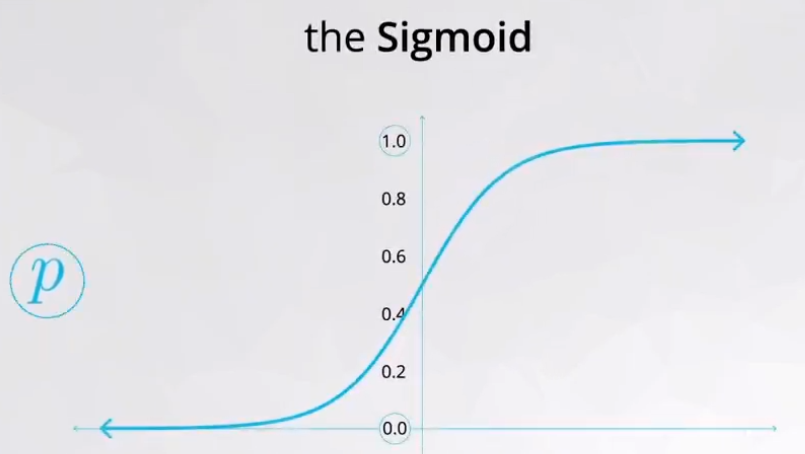
\includegraphics{01-img/c4_l16_01.png}
\caption{}
\end{figure}

Figure 1 - Sigmoid function.

Observe the two extreme values, 0 and 1, these two values will be used
to describe the two categories of the variable you want to predict.
Figure 2 shows an example.

\begin{figure}
\centering
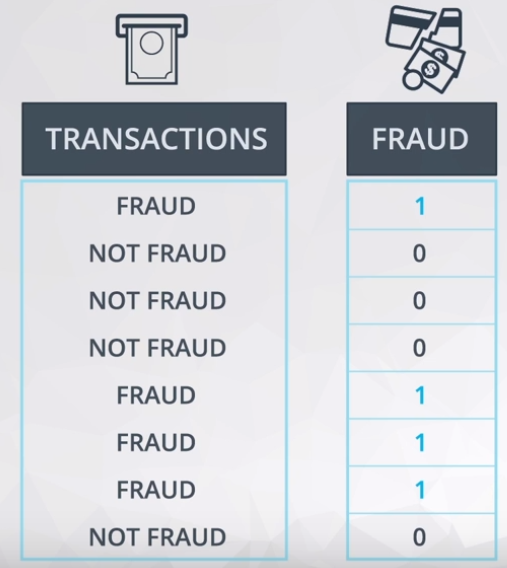
\includegraphics{01-img/c4_l16_02.png}
\caption{}
\end{figure}

Figure 2 - How to interpret the categories of Transactions column.

In other words, the outcome would be:

\[y \in \{0,1\}\]

Where:

\begin{itemize}
\tightlist
\item
  0: Positive class (Yes, Spam)
\item
  1: Negative class (No, Not spam)
\end{itemize}

The equation used in a regular Linear Regression is stated in equation
(1).

\[ y = a + b \cdot x_1 + c \cdot x_2   \tag{1}\]

Which could be noted as equation (2):

\[ \bold y = \underbrace{[a \ b \ c]}_{\theta^T} \cdot \underbrace{\begin{bmatrix} 1 \\ x_1 \\ x_2\end{bmatrix}}_{x} = \theta^T \cdot \bold x \tag{2}\]

The outcome \(\bold y\) could have any real number and this is the
reason to apply it to the sigmoid function, this action will delimited
the outcome between 0 and 1. Equantion (3) shows how is the sigmoid
function.

\[h_{\theta}(\bold y) = \frac{1}{1 + e^{- \bold y}} = \frac{1}{1 + e^{-\theta^T \bold x}}\]

Where:

\begin{itemize}
\tightlist
\item
  \(\theta^T:\) Coefficients of a linear regression;
\item
  \(\bold x:\)Training set.
\end{itemize}

Have in mind, the \(\bold y\) will be defined as:

\begin{itemize}
\tightlist
\item
  \(0.5 < \bold y \leq 1.0:\) round to 1;
\item
  \(0.0 \leq \bold y \leq 0.5:\) round to 0.
\end{itemize}

\subsubsection*{Interpretation}\label{interpretation-2}
\addcontentsline{toc}{subsubsection}{Interpretation}

The way to interpret the \texttt{coef} from the \texttt{.Logit()} is
quite different from the \texttt{.OLS()}. Figure 3 shows an example of
outcome from the Logistic Regression.

\begin{figure}
\centering
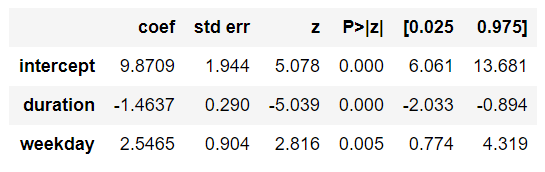
\includegraphics{01-img/c4_l16_03.png}
\caption{}
\end{figure}

Figure 3 - Example of Logistic Regression output.

Equally to the Multiple Linear Regression the baseline still in the
intercept, but the comparison is made by ``times''.

Recall, in this example \texttt{weekend} is the \texttt{baseline} .

For instance:

\[e^{2.5465} = 12.76 \text{ times} \]

This means:

\begin{quote}
On Weekdays the chance of fraud is 12.76 times more likely than on
weekends. Have in mind, the weekend is our baseline.
\end{quote}

It is not necessary to do math (add or subtract from the baseline).

\[e^{-1.4637} = 0.23 \text{ times} \]

This means:

\begin{quote}
For each minute spent in transaction the fraud is 0.23 times more likely
than on weekends.
\end{quote}

In this case, this kind of conclusion is quite wierd, and for this
reason we rephrase it.

\[1/e^{-1.4637} = 4.32 \text{ times} \]

\begin{quote}
For each minute less spent on the transaction, the chance of fraud is
4.32 times more likely holding the day of the week constant.
\end{quote}

\subsection{Model Diagnostic}\label{model-diagnostic}

The model diagnostic will be performed by the Confusion Matrix. Figure
4, 5, and 6 shows examples of this kind of matrix with differents
values.

\begin{figure}
\centering
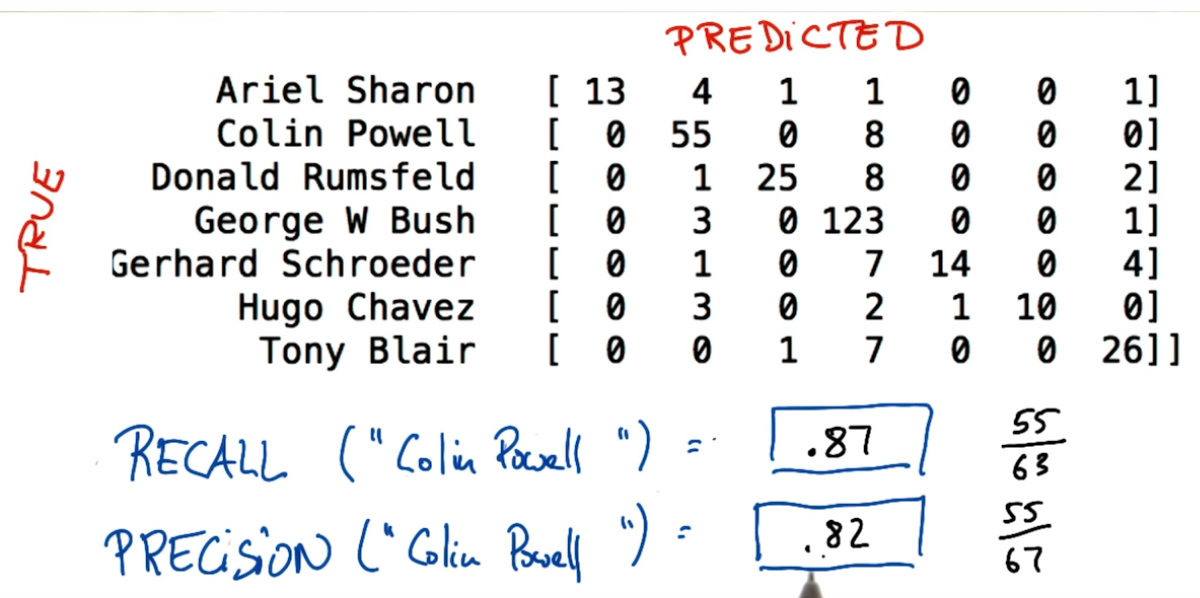
\includegraphics{01-img/c4_l16_04.png}
\caption{}
\end{figure}

Figure 4 - Confusion Matrix - Collin Powell Example.

\begin{figure}
\centering
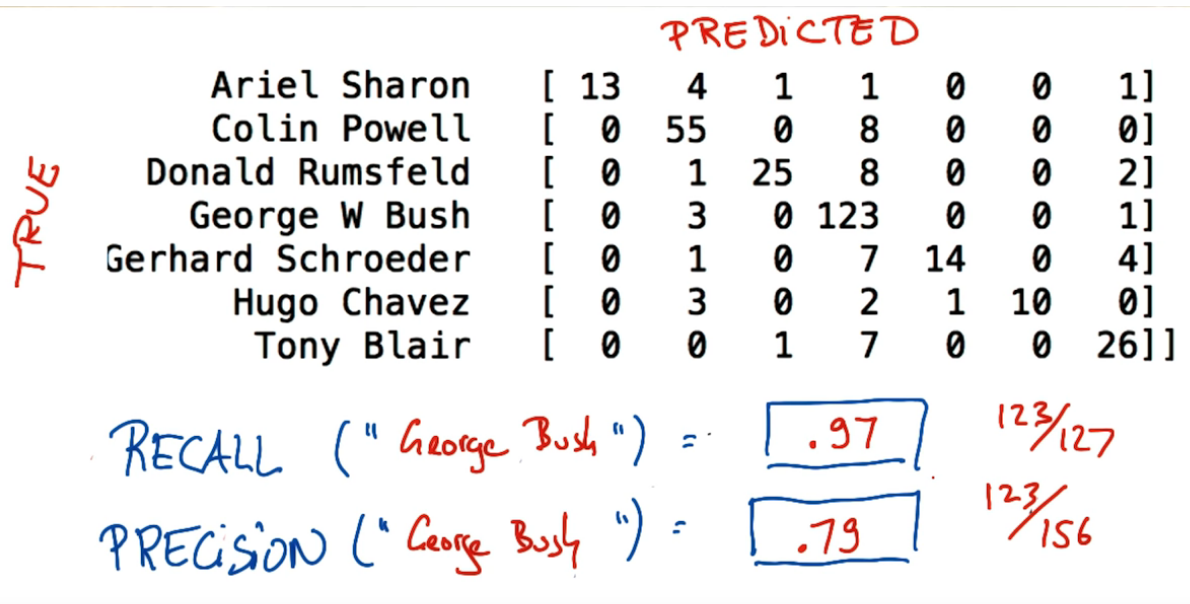
\includegraphics{01-img/c4_l16_05.png}
\caption{}
\end{figure}

Figure 5 - Confusion Matrix - George Bush Example.

\begin{figure}
\centering
\includegraphics{01-img/c4_l16_06.png}
\caption{}
\end{figure}

Figure 6 - Confusion Matrix - Donald Rumsfeld - Example.

Based on these example, recall and precision could be defined as:

\begin{itemize}
\tightlist
\item
  \textbf{Recall:} Out of all the items that are truly positive, how
  many were correctly classified as positive. Or simply, how many
  positive items were `recalled' from the dataset.
\end{itemize}

\[\text{Recall} = \frac{\text{True Positive}}{\text{True Positive + False Negative}}\]

\begin{itemize}
\tightlist
\item
  \textbf{Precision:} Out of all the items labeled as positive, how many
  truly belong to the positive class.
\end{itemize}

\[\text{Recall} = \frac{\text{True Positive}}{\text{True Positive + False Positive}}\]

\subsection{Statistics vs Machine
Learning}\label{statistics-vs-machine-learning}

\begin{figure}
\centering
\includegraphics{01-img/c4_l16_07.png}
\caption{}
\end{figure}

Figure 7 - Comparison between Statistics and Machine Learning.

\subsection{New Methods}\label{new-methods-1}

\subsubsection{\texorpdfstring{\texttt{.drop()}}{.drop()}}\label{drop}

This method drop a column, is a part of pandas.

\begin{Shaded}
\begin{Highlighting}[]
\NormalTok{pd.drop(}\StringTok{'column_to_be_dropped'}\NormalTok{, axis }\OperatorTok{=} \DecValTok{1}\NormalTok{)}
\end{Highlighting}
\end{Shaded}

\subsubsection{\texorpdfstring{\texttt{.Logit()}}{.Logit()}}\label{logit}

This method is anologous to the OLS and performs the Logistic
Regression.

\begin{Shaded}
\begin{Highlighting}[]
\ImportTok{import}\NormalTok{ statsmodels }\ImportTok{as}\NormalTok{ sm}

\NormalTok{sm.Logit(}\StringTok{'y_variable'}\NormalTok{, [}\StringTok{'intercept'}\NormalTok{,}\StringTok{'x1_variable'}\NormalTok{,}\StringTok{'x2_variable'}\NormalTok{])}
\end{Highlighting}
\end{Shaded}

\chapter{Intro to Machine Learning}\label{intro-to-machine-learning}

\section{Naïve Bayes}\label{naive-bayes}

Before dive in Naive Bayes. Let's talk a little bit about the thwo main
groups in Machine Learning.

\subsubsection*{Supervised Learning}\label{supervised-learning}
\addcontentsline{toc}{subsubsection}{Supervised Learning}

\begin{quote}
\textbf{In supervised learning, we are given a data set and already know
what our correct output should look like}, having the idea that there is
a relationship between the input and the output.

Supervised learning problems are categorized into ``regression'' and
``classification'' problems. In a regression problem, we are trying to
predict results within a continuous output, meaning that we are trying
to map input variables to some continuous function. In a classification
problem, we are instead trying to predict results in a discrete output.
In other words, we are trying to map input variables into discrete
categories.

Example 1:

Given data about the size of houses on the real estate market, try to
predict their price. Price as a function of size is a continuous output,
so this is a regression problem.

We could turn this example into a classification problem by instead
making our output about whether the house ``sells for more or less than
the asking price.'' Here we are classifying the houses based on price
into two discrete categories.

Example 2:

\begin{itemize}
\item
  Regression - Given a picture of a person, we have to predict their age
  on the basis of the given picture
\item
  Classification - Given a patient with a tumor, we have to predict
  whether the tumor is malignant or benign. ---
  \href{https://www.coursera.org/learn/machine-learning}{Coursera
  Machine Learning Notebook}
\end{itemize}
\end{quote}

\subsubsection*{Unsupervised Learning}\label{unsupervised-learning}
\addcontentsline{toc}{subsubsection}{Unsupervised Learning}

\begin{quote}
Unsupervised learning allows us to approach problems with little or no
idea what our results should look like. We can derive structure from
data where we don't necessarily know the effect of the variables.

We can derive this structure by clustering the data based on
relationships among the variables in the data.

With unsupervised learning there is no feedback based on the prediction
results.

Example:

Clustering: Take a collection of 1,000,000 different genes, and find a
way to automatically group these genes into groups that are somehow
similar or related by different variables, such as lifespan, location,
roles, and so on.

Non-clustering: The ``Cocktail Party Algorithm'', allows you to find
structure in a chaotic environment. (i.e.~identifying individual voices
and music from a mesh of sounds at a cocktail party). ---
\href{https://www.coursera.org/learn/machine-learning}{Coursera Machine
Learning Notebook}
\end{quote}

\subsection{Gaussian - Naive Bayes}\label{gaussian---naive-bayes}

\begin{quote}
In machine learning, naive Bayes classifiers are a family of simple
``probabilistic classifiers'' based on applying Bayes' theorem with
strong (naive) independence assumptions between the features. ---
\href{https://en.wikipedia.org/wiki/Naive_Bayes_classifier}{Wikipedia}
\end{quote}

The
\href{https://andersonuyekita.github.io/ND111_data_science_foundations_02/bayes-rule-lesson-07.html}{Naive
Bayes} was one of the topics covered in Advanced Statistics.

\subsection{Scikit Learn}\label{scikit-learn}

In this lesson we are going to use the scikit learn package to perform
the Gaussian Naive Bayes.

\begin{Shaded}
\begin{Highlighting}[]
\CommentTok{# Importing the library.}
\ImportTok{from}\NormalTok{ sklearn.naive_bayes }\ImportTok{import}\NormalTok{ GaussianNB}
\end{Highlighting}
\end{Shaded}

\subsubsection*{\texorpdfstring{\texttt{GaussianNB()}}{GaussianNB()}}\label{gaussiannb}
\addcontentsline{toc}{subsubsection}{\texttt{GaussianNB()}}

Creating the classifier.

\begin{Shaded}
\begin{Highlighting}[]
\CommentTok{# Creating the Classifier.}
\NormalTok{clf }\OperatorTok{=}\NormalTok{ GaussianNB()}
\end{Highlighting}
\end{Shaded}

\subsubsection*{\texorpdfstring{\texttt{.fit()}}{.fit()}}\label{fit}
\addcontentsline{toc}{subsubsection}{\texttt{.fit()}}

Bear in mind, the term \emph{fitting} or \emph{training} will be used
interchangeably along the course.

The \texttt{.fit()} method will be used to fit/train the classifier
based on two inputs:

\begin{itemize}
\tightlist
\item
  \textbf{X:} Coordinates/features of the variable to be classified;
\item
  \textbf{Y:} Results of already classified outputs.
\end{itemize}

Recall, this is a supervised algorithm, which means we have already some
results (that I do not care its origins) and what we are aiming is a
generalization of this classification using a algorithm to calculate our
own coefficients based on a training data.

An example of X and Y from Scikit Learning website:

\begin{Shaded}
\begin{Highlighting}[]
\CommentTok{### Inputs.}

\CommentTok{# This is the coordinates of each point.}
\NormalTok{X }\OperatorTok{=}\NormalTok{ np.array([[}\OperatorTok{-}\DecValTok{1}\NormalTok{, }\OperatorTok{-}\DecValTok{1}\NormalTok{], [}\OperatorTok{-}\DecValTok{2}\NormalTok{, }\OperatorTok{-}\DecValTok{1}\NormalTok{], [}\OperatorTok{-}\DecValTok{3}\NormalTok{, }\OperatorTok{-}\DecValTok{2}\NormalTok{], [}\DecValTok{1}\NormalTok{, }\DecValTok{1}\NormalTok{], [}\DecValTok{2}\NormalTok{, }\DecValTok{1}\NormalTok{], [}\DecValTok{3}\NormalTok{, }\DecValTok{2}\NormalTok{]])}

\CommentTok{# This is the outcome of each classification.}
\NormalTok{Y }\OperatorTok{=}\NormalTok{ np.array([}\DecValTok{1}\NormalTok{, }\DecValTok{1}\NormalTok{, }\DecValTok{1}\NormalTok{, }\DecValTok{2}\NormalTok{, }\DecValTok{2}\NormalTok{, }\DecValTok{2}\NormalTok{])}
\end{Highlighting}
\end{Shaded}

Plotting the X dataframe using the Y vector as categorical variable to
classify each point of X.

Figure 1 - X and Y plotted.

Now, I want to train my \texttt{clf} (classifier) based on X and Y to
classify any point.

\begin{Shaded}
\begin{Highlighting}[]
\CommentTok{# fit the classifier on the training features and labels}
\NormalTok{clf.fit(X, Y)}
\end{Highlighting}
\end{Shaded}

\begin{quote}
What is the classification for (-0.8, -1)?
\end{quote}

Let's take a look where is this point.

Figure 2 - New point in green.

Using the \texttt{.predict()} method it is possible to predict the
classification of this point.

\begin{Shaded}
\begin{Highlighting}[]
\NormalTok{clf.predict([[}\OperatorTok{-}\FloatTok{0.8}\NormalTok{, }\OperatorTok{-}\DecValTok{1}\NormalTok{]])}
\end{Highlighting}
\end{Shaded}

\begin{quote}
\textbf{The result is Type 1, as we expected to be.}
\end{quote}

Have in mind, generally we use two datasets:

\begin{itemize}
\tightlist
\item
  Training dataset: Used to train the model;
\item
  Test dataset: Used to test.
\end{itemize}

Training and Test datasests are complete different and it is necessary
to avoid overfitting. Recall, you will use the test dataset to calculate
the accuracy of your model.

\subsubsection{\texorpdfstring{\texttt{accuracy\_score()}}{accuracy\_score()}}\label{accuracy_score}

This method is used to calculate the model accuracy.

\begin{Shaded}
\begin{Highlighting}[]
\NormalTok{accuracy_score(y_true, y_pred)}
\end{Highlighting}
\end{Shaded}

Where:

\begin{itemize}
\tightlist
\item
  \texttt{y\_true:} True values;
\item
  \texttt{y\_pred:} Values predicted from the model, need to be check
  using the \texttt{y\_true}.
\end{itemize}

\subsection{Text Learning}\label{text-learning}

This is an application of the same package Scikit Learn, but this time
the problem is a bit more complicated.

Figure 3 shows, very simplified, the probability of each word given the
email writer.

Figure 3 - Probability diagram of Chris and Sara.

Suppose an email like this.

\[\text{Love life!} \tag{1}\]

\emph{What is the person more likely to be written this email?}

Given the probability of Chris and Sara is equal to 50\%.

\begin{itemize}
\tightlist
\item
  \(P(Chris) = P(Sara) = 0.5\)
\end{itemize}

This is the \emph{a priori} probabilities.

Based on the probabilities in Figure 3, let's calculate the \emph{joint}
probabilities.

\begin{itemize}
\tightlist
\item
  \(P_{chris,\text{Love life}} = 0.1 \cdot 0.1 \cdot 0.5 = 0.005\)
\item
  \(P_{sara,\text{Love life}} = 0.5 \cdot 0.3 \cdot 0.5 = 0.075\)
\end{itemize}

A new email like this:

\[\text{Life deal} \tag{2}\]

\begin{itemize}
\tightlist
\item
  \(P_{chris,\text{Life deal}} = 0.1 \cdot 0.8 \cdot 0.5 = 0.004\)
\item
  \(P_{sara,\text{Life deal}} = 0.3 \cdot 0.2 \cdot 0.5 = 0.003\)
\end{itemize}

Founded on the \emph{joint} probabilities, we can calculate the
\emph{normalizator} (:)) of probabilities.

\begin{itemize}
\tightlist
\item
  For \(\text{Love life!}\);
\end{itemize}

\[P(\text{Love life}) = P(chris) \cdot P_{chris,\text{Love life}} + P(sara) \cdot P_{sara,\text{Love life}} = P(chris) \cdot 0.08\]

\begin{itemize}
\tightlist
\item
  For \(\text{Life deal}\);
\end{itemize}

\[P(\text{Life deal}) = P(chris) \cdot P_{chris,\text{Life deal}} + P(sara) \cdot P_{sara,\text{Life deal}} = 0.007\]

Finally, using \emph{normalizator} and \emph{joint} probabilities we can
calculate the \emph{a posteriori} probabilities.

\begin{itemize}
\tightlist
\item
  For \(\text{Love life!}\);
\end{itemize}

Using the \(P(\text{Love life})\) to normalize
\(P_{chris,\text{Love life}}\) and \(P_{sara,\text{Love life}}\):

\[P(\text{Chris|"Love life"}) = P(chris) \cdot \frac{P_{chris,\text{Love life}}}{P(chris) \cdot P(\text{Love life})} = \frac{0.005}{0.080} = 0.0625\]

\[P(\text{Sara|"Love life"}) = P(sara) \cdot \frac{P_{sara,\text{Love life}}}{P(sara) \cdot P(\text{Love life})} = \frac{0.075}{0.080} = 0.9375\]

\begin{itemize}
\tightlist
\item
  For \(\text{Life deal}\);
\end{itemize}

Using the \(P(\text{Life deal})\) to normalize
\(P_{chris,\text{Life deal}}\) and \(P_{sara,\text{Life deal}}\):

\[P(\text{Chris|"Life deal"}) = P(chris) \cdot \frac{P_{chris,\text{Life deal}}}{P(chris) \cdot P(\text{Life deal})} = \frac{0.004}{0.007} = 0.5714\]

\[P(\text{Sara|"Life deal"}) = P(sara) \cdot \frac{P_{sara,\text{Life deal}}}{P(sara) \cdot P(\text{Life deal})} = \frac{0.003}{0.007} = 0.4286\]

\section{Support Vector Machine (SVM)}\label{support-vector-machine-svm}

The Support Vector Machine was an algorithm invented by
\href{https://en.wikipedia.org/wiki/Support-vector_machine}{Hava
Siegelmann and Vladimir Vapnik}. The objective of this algorithm is to
fit a line to divide a group of point/features in two or more classes.

Figure 1 show the possibilities the line to segregate the two types of
points.

Figure 1 - Possible lines to divide the points in two groups.

All the three lines could be a solution, but the SMV algorithm aims to
maximaze the distance to the nearest point, which is the so-called
\textbf{margin}.

Have in mind, the first objective of SMV is to classify correctly, later
maximize the \textbf{margin}.

\subsubsection*{Additional notebooks}\label{additional-notebooks}
\addcontentsline{toc}{subsubsection}{Additional notebooks}

For a better understanding about SVM, read the \href{a}{bookdown of
Machine Learning} offered by Stanford and taught by Andrew Ng.

This course is focused in application and do not talk much about the
theoretical aspects.

\subsection{Scikit Learn}\label{scikit-learn-1}

The Scikit Learn also has methods to calculate the SVM.

\subsubsection{\texorpdfstring{\texttt{SVC()}}{SVC()}}\label{svc}

This function creates an object classifier.

\begin{Shaded}
\begin{Highlighting}[]
\NormalTok{clf }\OperatorTok{=}\NormalTok{ SVC(kernel }\OperatorTok{=} \StringTok{'linear'}\NormalTok{)}
\end{Highlighting}
\end{Shaded}

Remember, the \texttt{kernel} used is linar, which means the SVM will
plot a straight line, and also could be lon-linear.

\subsubsection{Non linear SVM}\label{non-linear-svm}

The non-linear SVM occurs when you adopt a non-linear kernel, as you can
see in Figure 2.

Figure 2 - Example of Non-linear SVM.

There are several non-linear kernels:

\begin{itemize}
\tightlist
\item
  Poly;
\item
  rbf (gives the curvy answer);
\item
  Sigmoid, etc.
\end{itemize}

The uses of a polynomial gives the output of Figure 3.

Figure 3 - Interpretation of \(z = x^2 + y^2\).

\subsubsection{Parameters}\label{parameters}

This is characteristics that you define when you creating the
classifier, so before you fitting the data. There are three:

\begin{itemize}
\tightlist
\item
  Kernel;
\item
  Gamma, and;
\item
  C.
\end{itemize}

Figure 4 shows two examples of output with different kernel.

Figure 4 - Comparison between linear (on the left side) and rbf (on the
right side).

For this reason, the kernel could change completely the boundary.

\begin{Shaded}
\begin{Highlighting}[]
\NormalTok{clf }\OperatorTok{=}\NormalTok{ sm.SVC(C }\OperatorTok{=} \DecValTok{1}\NormalTok{, gamma }\OperatorTok{=} \DecValTok{1}\NormalTok{, kernel }\OperatorTok{=} \StringTok{"rbf"}\NormalTok{)}
\end{Highlighting}
\end{Shaded}

\subsubsection{C}\label{c}

Controls trafeoff between smooth decision boundary and classifying
training points correctly.

\begin{quote}
A low C makes the decision surface smooth, while a high C aims at
classifying all training examples correctly.
\end{quote}

\subsubsection{Gamma}\label{gamma}

Defines how far the influence of a single training example reaches.

\begin{quote}
gamma defines how much influence a single training example has. The
larger gamma is, the closer other examples must be to be affected.
\end{quote}

\subsubsection{Overfitting}\label{overfitting}

Avoide the overfitting, in SVM there are three parameters which could
lead overfitting.

\begin{itemize}
\tightlist
\item
  Kernel;
\item
  C
\item
  gamma
\end{itemize}

\subsubsection{\texorpdfstring{\texttt{.fit()}}{.fit()}}\label{fit-1}

Similarly to the \texttt{.fit()} from GaussianNB.

\begin{Shaded}
\begin{Highlighting}[]
\CommentTok{# Fitting a model.}
\NormalTok{clf.fit(X_train,Y_train)}
\end{Highlighting}
\end{Shaded}

Where:

\begin{itemize}
\tightlist
\item
  X\_train: is the ``coordinates'' of the points to train the data;
\item
  Y\_train: the answer of each pair of coordinates.
\end{itemize}

\subsubsection{\texorpdfstring{\texttt{.pred()}}{.pred()}}\label{pred}

Based on the \texttt{clf} it is possible to predict the values of a test
dataframe.

\begin{Shaded}
\begin{Highlighting}[]
\CommentTok{# After fitting the clf you can use to predict.}
\NormalTok{clf.pred(X_test)}
\end{Highlighting}
\end{Shaded}

\section{Decision Trees}\label{decision-trees}

\begin{quote}
A decision tree is a decision support tool that uses a tree-like model
of decisions and their possible consequences, including chance event
outcomes, resource costs, and utility. It is one way to display an
algorithm that only contains conditional control statements.

Decision trees are commonly used in operations research, specifically in
decision analysis, to help identify a strategy most likely to reach a
goal, but are also a popular tool in machine learning. ---
\href{https://en.wikipedia.org/wiki/Decision_tree}{Wikipedia}
\end{quote}

In Scikit Learn you can also find the Decision Trees.

\subsection{Scikit Learn Decision
Tree}\label{scikit-learn-decision-tree}

This classifier has the same workflow from the other two (GaussianNB and
SVM).

\begin{Shaded}
\begin{Highlighting}[]
\CommentTok{# Import decision tree from sklearn.}
\ImportTok{from}\NormalTok{ sklearn }\ImportTok{import}\NormalTok{ tree}

\CommentTok{# Create the classifier using tree.}
\NormalTok{clf }\OperatorTok{=}\NormalTok{ tree.DecisionTreeClassifier()}

\CommentTok{# Fitting/Training the model.}
\NormalTok{clf.fit(df_train, labels_train)}

\CommentTok{# Predicting}
\NormalTok{pred }\OperatorTok{=}\NormalTok{ clf.predict(df_test)}
\end{Highlighting}
\end{Shaded}

\subsection{Parameters}\label{parameters-1}

The \texttt{.DecisionTreeClassifier()} has a lot of parameters to set
up.

\subsubsection{\texorpdfstring{\texttt{min\_samples\_split}}{min\_samples\_split}}\label{min_samples_split}

This parameter set a limit of how deep the decision tree will go. Figure
1 shows an example of the extension of the Tree.

Figure 1 - Example of leafs and nodes.

As you can see the \texttt{min\_samples\_split} will go further for each
node until reach the node with two leafs.

The effect of going further and further, it means, a very low number of
\texttt{min\_samples\_split} is more likely prone to overfitting. You
can see an example of overfitting in Figure 2.

Figure 2 - Overfitting.

\subsubsection{Entropy}\label{entropy}

Bear in mind, the default function to measure the quality of a split in
\texttt{DecisionTreeClassifier()} is the \texttt{gini}index instead of
the \texttt{entropy}.

The entropy controls how the decision tree decides where to split the
data.

\[entropy = - \sum_i^n p_i \cdot (\ln(p_i))\]

When entropy is 1 there is no pattern, the data was spread equally on
the ``plot'' and you can not realize where to split. On the other hand,
when entropy is 0 there are a clearly areas to split.

Though, the entropy is applied to parents and child of the tree in a way
that you will ``compare'' entropies from parents and child.

\subsubsection{Gain}\label{gain}

Founded on the entropies calculated from the parent and child, it is
possible to calculate the gain.

\[\text{Information Gain} = entropy(parent) - [\text{weighted average]} \cdot entropy(children)\]

Figure 3 - Information Gain.

The object function of a decision tree is to maximize the information
gain.

\subsubsection{Example}\label{example}

Figure 4 shows a dataframe to be splited.

Figure 4 - How to split using Decision Tree?.

Bear in mind, the parent entropy of the all dataset is 1.

Now, let's use the \textbf{gain information} to decide which variable to
use.

\textbf{Grade}

Ilustrating the decision tree using a tree, Figure 5 shows a summary.

Figure 5 - The grade splitting.

Splitting by grade flat has only fast, whereas steep has two slow and 1
gast. Let's calculate the probabilities/proportion in Table 1:

Table 1 - Table of quantity and proportion for Grade

\begin{longtable}[]{@{}ccccc@{}}
\toprule
& Steep & Flat & psteep & pflat\tabularnewline
\midrule
\endhead
Slow & 2 & 1 & 2/3 & 1/3\tabularnewline
Fast & 0 & 1 & 0/1 & 1/1\tabularnewline
\bottomrule
\end{longtable}

Based on these probabilities, I can calculate the entropy of each
category (steep and flat).

\begin{itemize}
\tightlist
\item
  Entropy calculation:
\end{itemize}

\[entropy(flat) = -(p_{flat,slow} \cdot \ln(p_{flat,slow}) + p_{flat,fast} \cdot \ln(p_{flat,fast})) = \\ -(1 \cdot \ln(1) + 0 \cdot \ln(0)) = 0 \]

\[entropy(steep) = -(p_{steep,slow} \cdot \ln(p_{steep,slow}) + p_{steep,fast} \cdot \ln(p_{steep,fast})) = -(\frac{2}{3} \cdot \ln(\frac{2}{3}) + \frac{1}{3} \cdot \ln(\frac{1}{3})) = 0.9183\]

\begin{itemize}
\tightlist
\item
  Information Gain:
\end{itemize}

\[\text{Information Gain} = 1 - (0.9182 \cdot \frac{3}{4} + 0 \cdot \frac{1}{4}) = 0.3112 \]

\begin{quote}
The Gain of Information is 0.3112
\end{quote}

Table 2 - Table of quantity and proportion for Bumpiness

\begin{longtable}[]{@{}ccccc@{}}
\toprule
& Steep & Flat & psteep & pflat\tabularnewline
\midrule
\endhead
Bumpy & 1 & 1 & 1/2 & 1/2\tabularnewline
Smooth & 1 & 1 & 1/2 & 1/2\tabularnewline
\bottomrule
\end{longtable}

\begin{itemize}
\tightlist
\item
  Entropy calculation:
\end{itemize}

\[entropy(bumpy) = -(p_{bumpy,slow} \cdot \ln(p_{bumpy,slow}) + p_{bumpy,fast} \cdot \ln(p_{bumpy,fast})) = \\ -(0.5 \cdot \ln(0.5) + 0.5 \cdot \ln(0.5)) = 1 \]

\[entropy(smooth) = -(p_{smooth,slow} \cdot \ln(p_{smooth,slow}) + p_{smooth,fast} \cdot \ln(p_{smooth,fast})) = -(0.5 \cdot \ln(0.5) + 0.5 \cdot \ln(0.5)) = 1 \]

\begin{itemize}
\tightlist
\item
  Information Gain:
\end{itemize}

\[\text{Information Gain} = 1 - (1 \cdot \frac{2}{4} + 1 \cdot \frac{2}{4}) = 0\]

\begin{quote}
For this variable there is no Gain of Information, which means we do not
learn anything splitting by bumpiness.
\end{quote}

Table 3 - Table of quantity and proportion for Speed Limit

\begin{longtable}[]{@{}ccccc@{}}
\toprule
& Steep & Flat & psteep & pflat\tabularnewline
\midrule
\endhead
yes & 2 & 0 & 2/2 & 0/2\tabularnewline
no & 0 & 2 & 0/2 & 2/2\tabularnewline
\bottomrule
\end{longtable}

\begin{itemize}
\tightlist
\item
  Entropy Calculation:
\end{itemize}

\[entropy(yes) = -(p_{yes,slow} \cdot \ln(p_{yes,slow}) + p_{yes,fast} \cdot \ln(p_{yes,fast})) = \\ -(1 \cdot \ln(1) + 0 \cdot \ln(0)) = 0 \]

\[entropy(no) = -(p_{no,slow} \cdot \ln(p_{no,slow}) + p_{no,fast} \cdot \ln(p_{no,fast})) = -(0 \cdot \ln(0) + 1 \cdot \ln(1)) = 0 \]

\begin{itemize}
\tightlist
\item
  Information Gain:
\end{itemize}

\[\text{Information Gain} = 1 - (1 \cdot 0 + 1 \cdot 0) = 1\]

\begin{quote}
Best information gain possible. You should split using this feature.
\end{quote}

Figure 6 - Speed Limit Decision Tree.

\subsubsection{Bias}\label{bias}

Bias in machine learning, means an algorithm that almost ``ignores'' the
data, it has almost no capacity to learn anything.

On the other hand, a machine learning very perceptive to data, will only
replicate what it has seen before, it has no capacity to ``generalize''
a new situation. It is called algorithm with high variance.

What we are looking for is something in the middle of bias and high
variance. This is the trade-off of bias-variance.

\section{Decision Trees}\label{decision-trees-1}

\begin{quote}
A decision tree is a decision support tool that uses a tree-like model
of decisions and their possible consequences, including chance event
outcomes, resource costs, and utility. It is one way to display an
algorithm that only contains conditional control statements.

Decision trees are commonly used in operations research, specifically in
decision analysis, to help identify a strategy most likely to reach a
goal, but are also a popular tool in machine learning. ---
\href{https://en.wikipedia.org/wiki/Decision_tree}{Wikipedia}
\end{quote}

In Scikit Learn you can also find the Decision Trees.

\subsection{Scikit Learn Decision
Tree}\label{scikit-learn-decision-tree-1}

This classifier has the same workflow from the other two (GaussianNB and
SVM).

\begin{Shaded}
\begin{Highlighting}[]
\CommentTok{# Import decision tree from sklearn.}
\ImportTok{from}\NormalTok{ sklearn }\ImportTok{import}\NormalTok{ tree}

\CommentTok{# Create the classifier using tree.}
\NormalTok{clf }\OperatorTok{=}\NormalTok{ tree.DecisionTreeClassifier()}

\CommentTok{# Fitting/Training the model.}
\NormalTok{clf.fit(df_train, labels_train)}

\CommentTok{# Predicting}
\NormalTok{pred }\OperatorTok{=}\NormalTok{ clf.predict(df_test)}
\end{Highlighting}
\end{Shaded}

\subsection{Parameters}\label{parameters-2}

The \texttt{.DecisionTreeClassifier()} has a lot of parameters to set
up.

\subsubsection{\texorpdfstring{\texttt{min\_samples\_split}}{min\_samples\_split}}\label{min_samples_split-1}

This parameter set a limit of how deep the decision tree will go. Figure
1 shows an example of the extension of the Tree.

Figure 1 - Example of leafs and nodes.

As you can see the \texttt{min\_samples\_split} will go further for each
node until reach the node with two leafs.

The effect of going further and further, it means, a very low number of
\texttt{min\_samples\_split} is more likely prone to overfitting. You
can see an example of overfitting in Figure 2.

Figure 2 - Overfitting.

\subsubsection{Entropy}\label{entropy-1}

Bear in mind, the default function to measure the quality of a split in
\texttt{DecisionTreeClassifier()} is the \texttt{gini}index instead of
the \texttt{entropy}.

The entropy controls how the decision tree decides where to split the
data.

\[entropy = - \sum_i^n p_i \cdot (\ln(p_i))\]

When entropy is 1 there is no pattern, the data was spread equally on
the ``plot'' and you can not realize where to split. On the other hand,
when entropy is 0 there are a clearly areas to split.

Though, the entropy is applied to parents and child of the tree in a way
that you will ``compare'' entropies from parents and child.

\subsubsection{Gain}\label{gain-1}

Founded on the entropies calculated from the parent and child, it is
possible to calculate the gain.

\[\text{Information Gain} = entropy(parent) - [\text{weighted average]} \cdot entropy(children)\]

Figure 3 - Information Gain.

The object function of a decision tree is to maximize the information
gain.

\subsubsection{Example}\label{example-1}

Figure 4 shows a dataframe to be splited.

Figure 4 - How to split using Decision Tree?.

Bear in mind, the parent entropy of the all dataset is 1.

Now, let's use the \textbf{gain information} to decide which variable to
use.

\textbf{Grade}

Ilustrating the decision tree using a tree, Figure 5 shows a summary.

Figure 5 - The grade splitting.

Splitting by grade flat has only fast, whereas steep has two slow and 1
gast. Let's calculate the probabilities/proportion in Table 1:

Table 1 - Table of quantity and proportion for Grade

\begin{longtable}[]{@{}ccccc@{}}
\toprule
& Steep & Flat & psteep & pflat\tabularnewline
\midrule
\endhead
Slow & 2 & 1 & 2/3 & 1/3\tabularnewline
Fast & 0 & 1 & 0/1 & 1/1\tabularnewline
\bottomrule
\end{longtable}

Based on these probabilities, I can calculate the entropy of each
category (steep and flat).

\begin{itemize}
\tightlist
\item
  Entropy calculation:
\end{itemize}

\[entropy(flat) = -(p_{flat,slow} \cdot \ln(p_{flat,slow}) + p_{flat,fast} \cdot \ln(p_{flat,fast})) = \\ -(1 \cdot \ln(1) + 0 \cdot \ln(0)) = 0 \]

\[entropy(steep) = -(p_{steep,slow} \cdot \ln(p_{steep,slow}) + p_{steep,fast} \cdot \ln(p_{steep,fast})) = -(\frac{2}{3} \cdot \ln(\frac{2}{3}) + \frac{1}{3} \cdot \ln(\frac{1}{3})) = 0.9183\]

\begin{itemize}
\tightlist
\item
  Information Gain:
\end{itemize}

\[\text{Information Gain} = 1 - (0.9182 \cdot \frac{3}{4} + 0 \cdot \frac{1}{4}) = 0.3112 \]

\begin{quote}
The Gain of Information is 0.3112
\end{quote}

Table 2 - Table of quantity and proportion for Bumpiness

\begin{longtable}[]{@{}ccccc@{}}
\toprule
& Steep & Flat & psteep & pflat\tabularnewline
\midrule
\endhead
Bumpy & 1 & 1 & 1/2 & 1/2\tabularnewline
Smooth & 1 & 1 & 1/2 & 1/2\tabularnewline
\bottomrule
\end{longtable}

\begin{itemize}
\tightlist
\item
  Entropy calculation:
\end{itemize}

\[entropy(bumpy) = -(p_{bumpy,slow} \cdot \ln(p_{bumpy,slow}) + p_{bumpy,fast} \cdot \ln(p_{bumpy,fast})) = \\ -(0.5 \cdot \ln(0.5) + 0.5 \cdot \ln(0.5)) = 1 \]

\[entropy(smooth) = -(p_{smooth,slow} \cdot \ln(p_{smooth,slow}) + p_{smooth,fast} \cdot \ln(p_{smooth,fast})) = -(0.5 \cdot \ln(0.5) + 0.5 \cdot \ln(0.5)) = 1 \]

\begin{itemize}
\tightlist
\item
  Information Gain:
\end{itemize}

\[\text{Information Gain} = 1 - (1 \cdot \frac{2}{4} + 1 \cdot \frac{2}{4}) = 0\]

\begin{quote}
For this variable there is no Gain of Information, which means we do not
learn anything splitting by bumpiness.
\end{quote}

Table 3 - Table of quantity and proportion for Speed Limit

\begin{longtable}[]{@{}ccccc@{}}
\toprule
& Steep & Flat & psteep & pflat\tabularnewline
\midrule
\endhead
yes & 2 & 0 & 2/2 & 0/2\tabularnewline
no & 0 & 2 & 0/2 & 2/2\tabularnewline
\bottomrule
\end{longtable}

\begin{itemize}
\tightlist
\item
  Entropy Calculation:
\end{itemize}

\[entropy(yes) = -(p_{yes,slow} \cdot \ln(p_{yes,slow}) + p_{yes,fast} \cdot \ln(p_{yes,fast})) = \\ -(1 \cdot \ln(1) + 0 \cdot \ln(0)) = 0 \]

\[entropy(no) = -(p_{no,slow} \cdot \ln(p_{no,slow}) + p_{no,fast} \cdot \ln(p_{no,fast})) = -(0 \cdot \ln(0) + 1 \cdot \ln(1)) = 0 \]

\begin{itemize}
\tightlist
\item
  Information Gain:
\end{itemize}

\[\text{Information Gain} = 1 - (1 \cdot 0 + 1 \cdot 0) = 1\]

\begin{quote}
Best information gain possible. You should split using this feature.
\end{quote}

Figure 6 - Speed Limit Decision Tree.

\subsubsection{Bias}\label{bias-1}

Bias in machine learning, means an algorithm that almost ``ignores'' the
data, it has almost no capacity to learn anything.

On the other hand, a machine learning very perceptive to data, will only
replicate what it has seen before, it has no capacity to ``generalize''
a new situation. It is called algorithm with high variance.

What we are looking for is something in the middle of bias and high
variance. This is the trade-off of bias-variance.

\chapter{Data Visualization
(Optional)}\label{data-visualization-optional}

We have finished a nice book.

\bibliography{book.bib,packages.bib}


\end{document}
